
% -----------------------------------------------------------------------
% Python Tutorial
% WS 18/19
% -----------------------------------------------------------------------
\documentclass[enabledeprecatedfontcommands, fontsize=12pt,
     open=right, a4paper,
     twoside, DIV=11,
     abstractoff,
     headsepline,
     numbers=noenddot,
     BCOR=15mm,
     headings=standardclasses,
     headings=big]{scrbook}
\KOMAoptions{cleardoublepage=empty}
% Header f�r Variablen
% Variablen
\newcommand{\theSemester}{Sommersemester 2019}
% Variable f�r die Vorlesung
\newcommand{\theProject}{}
% Variable f�r den Studiengang
\newcommand{\theTitle}{Python}
% Variable f�r den Hochschul-Namen
\newcommand{\theSchool}{Hochschule Kaiserslautern}
% Variable f�r den Dozenten
\newcommand{\theAuthor}{
    Julian  Bernhart,
    Manfred Brill,
    Eric Brunk,
    Mathias Fedder,
    Christopher Gross,
    Robin Guth,
    Rainer Haffner,
    Matthias Haselmaier,
 %   Kathrin Hentschel,
    Fabian Kalweit,
    Lukas Kuhn,
    Kevin Konrad,
    Philipp Lauer,
    Miriam Lohm�ller,
    Sebastian Morsch,
    Anatoli Sch�fer,
    Denis Schlusche,
    Christoph Seibel,
    Marc Zintel
}

%
% ----------------------------------------------------------------------------------------------
% Vorlage f�r Dokumentation auf LaTeX-Basis im Projekt InfoStuDi
% --------------------------------------------------------------------------------------------
\usepackage{mb}
\usepackage{mbmath}
\usepackage{textcomp}
\usepackage{german}
% Array-Paket f�r mehr Kontrolle der Tabellen
\usepackage{array}
% ifthen f�r Ein- und Ausblenden der L�sungen.
\usepackage{ifthen}
% Paket f�r Postscript Pi-Fonts
\usepackage{pifont}
% PSTricks
%\usepackage{pstricks}
% Paket f�r das einfache Umdefinieren von Listen
\usepackage[shortlabels]{enumitem}
% Alphabetischer Index
\usepackage{imakeidx}
\makeindex[title=Index,columns=2,options=-s german,intoc]
% Header und Footer mit KomaScript
\usepackage[automark, headsepline]{scrlayer-scrpage}
% Caption unteraderm, dass \ref nicht nur zur Caption sondern auch zur Figure springt
\usepackage{caption}
%
% Header f�r Werkzeuge, Begriffe aus dem Software-Management
\input{variablen}
% Farben
\input{colors}
% Standardverzeichnis f�r das Basisverzeichnis der Bilder
%
\newcommand{\imagePath}{./images}
%
\raggedbottom
\setlength{\parskip}{2.0ex}
\setlength{\parindent}{0.0cm}
%% Verhindert Schusterjungen und Hurenkinder
\clubpenalty = 10000
\widowpenalty = 10000 \displaywidowpenalty = 10000
%
\setcounter{secnumdepth}{2}
\setcounter{tocdepth}{2}
%
\pagestyle{scrheadings}
\clearscrheadfoot
% Thema des Dokuments in die Kopfzeile
\ihead{\headmark}
\ohead[]{\pagemark}
\chead{}
\pagestyle{scrheadings}
% Abst�nde zwischen Caption und Bild/Tabelle
\setlength\abovecaptionskip          {0.4em}
\setlength\belowcaptionskip          {0.2em}
% Anteil der Grafiken h�her auf jeder Seite!
\renewcommand{\textfraction}{0.001}
\renewcommand{\topfraction}{0.99}
% Literatur-Stil
\bibliographystyle{geralpha}
% Listingspaket
\usepackage{listings}
\lstloadlanguages{python}
\lstset{language=python}
\definecolor{lstback}{gray}{0.85}
\lstset{backgroundcolor=\color{lstback}}
\lstset{extendedchars=true}
\lstset{showstringspaces = false}
\lstset{basicstyle = \ttfamily \small}
%% listings mit listings.sty
%
% Kommando f�r den Flattersatz bei nebeneinander liegenden Abbildungen
\newcommand{\flatter}{\setlength{\rightskip}{0pt plus 2cm}}
%
% Schritte in einer Aufz�hlung, daf�r einen Z�hler (schritt) und die Umgebung
% schritte definieren.
\newcounter{schritt}
\newenvironment{schritte}%
{\begin{list}%
{Schritt \arabic{schritt}:}%
{\usecounter{schritt}\settowidth{\labelwidth}{Schritt 1:}%
\setlength{\leftmargin}{\labelwidth}\addtolength\leftmargin{\labelsep}%
\parsep0.0ex\partopsep-0.3ex\itemsep2pt\topsep0.0ex}}{\end{list}}
% Dateinamen f�r interne Musterl�sungen
\newcommand{\filename}[1]{%
\ifthenelse{\boolean{solutions}}{\framebox[50mm]{\parbox{40mm}{\textbf #1}}\vspace{6pt}}{}}
%   Taste
\newcommand{\taste}[1]{\small\textsf{#1}\normalsize}
%   gesch�tzte Namen (NICHT in chapter, section usw. verwenden!)
\newcommand{\name}[1]{\textsl{#1}}
%   Fachbegriffe/Erkl�rung von Abk�rzungen
\newcommand{\begriff}[1]{\index{#1}\textit{#1}}
%
\newcommand{\algorithmus}[2]{%
\vspace{4pt}\fboxsep 1mm \framebox[140mm]
{\parbox{135mm}{{\textbf{#1}}\vspace{2pt}#2}}\vspace{4pt}}
%
%   Dateinamen/Pfade
\newcommand{\datei}[1]{\texttt{#1}\normalsize}
%   Tip (in einer Box)
\newcommand{\tip}[1]{%
\vspace{4pt}\fboxsep 1mm \framebox[140mm]
{\parbox{135mm}{{\textbf{Tipp}}:\\ #1}}\vspace{4pt}}

%Achtung in einer Box
\newcommand{\warning}[1]{%
    \par\vspace{4pt}\fboxsep 1mm \framebox[140mm]%
    {\parbox{135mm}{{\textbf{Achtung}}:\\ #1}}\vspace{4pt}%
}
%

%
%   Reflektion (in einer Box)
%
\newcommand{\reflection}[1]{
\begin{quote}\fboxsep 3mm\framebox[140mm][c]{\parbox{130mm}{{\textbf{Reflektion}:\\}#1}}\end{quote}}
%
%   Angabe, was die Studierenden lesen sollen (in einer Box)

\newcommand{\lesen}[1]{%
\begin{minipage}[c]{2.5cm}
\centering
\includegraphics[width=2cm]{\imagePath/Misc/buchicon}%
\end{minipage}%
\begin{minipage}[t]{12cm}%
#1%
\end{minipage}}
%
%   Angabe im Begleittext, was die Studierenden lesen sollen (in einer Box)
%   Dieses Icon wird f�r Angaben verwendet, die nicht verpflichtend zu lesen
%   sind. Also "nice-to-have", "wenn sie noch Zeit haben".
\newcommand{\vertiefen}[1]{%
\begin{minipage}[b]{2.5cm}
\centering
\includegraphics[width=2cm]{\imagePath/Misc/reading}%
\end{minipage}%
\begin{minipage}[b\newcommand{\firefox}{\texttt{Mozilla Firefox}}
\newcommand{\kde}{\texttt{KDE}}]{12cm}%
#1%
\end{minipage}}
%
% Jetzt kommt die Definition der Kontrollfrage; die Nummerierung
% f�r das ganze erhalten wir mit Hilfe von \item{\kontroll}.
%
% Ein Counter f�r die Kontrollfragen. Wir z�hlen diesen Counter selbst hoch
% mit einem entsprechenden Kommando, das wir in \item verwenden.
% 1
\newcounter{kontrollCounter}[section]
\newcommand{\kontroll}[0]{
    \refstepcounter{kontrollCounter}
    % Kapitelnummer.Z�hler f�r das Item
    \arabic{chapter}.\arabic{kontrollCounter}
    % Das Label ist bis auf weiteres "kontrolle:Kapitelnummer:kontrollcounter
    \label{kontrolle:\arabic{chapter}:\arabic{kontrollCounter}}
}
% Jetzt kommt die Definition der Kontrollfrage; die Nummerierung
% f�r das ganze erhalten wir mit Hilfe von \item{\kontroll}.
\newcommand{\kontrollfrage}[1]{%
\begin{minipage}[c]{1.85cm}
\huge{\ding{46}}%
\end{minipage}%
\begin{minipage}[t]{12cm}%
\begin{itemize}#1%
\end{itemize}%
\end{minipage}}
%
% Einblenden von Musterl�sungen
%
% Schalter f�r das ein- und ausblenden der L�sungen
\newboolean{solutions}
%
% Theorem-Umgebung f�r die �bungsaufgaben
% Wichtig: alle Attribute einstellen, dann die neue
% theorem-Umgebung mit newtheorem definieren!
% Oder, wie hier, durch das Einschlie�en in {}
%
{
% Zeilenumbruch bei Aufgaben-�berschrift
\theoremstyle{break}
% "Normaler" Font im Text
\theorembodyfont{\normalfont}
% Kapitelweise neu nummerieren
% 2
\newtheorem{auftitle}{Aufgabe}[section]
}
%
% Definition f�r die Kennzeichnung der �bungsaufgaben
%
\newcommand{\uebung}{%
\vspace*{11pt}%
\begin{tabular}{@{}p{2.25cm}@{}p{11.7cm}}%
\huge{\ding{45}}&\Large{\textbf{�bungsaufgaben}}%
\end{tabular}%
}
% Ein Counter f�r die �bungsaufgaben. Wir z�hlen diesen Counter selbst hoch
% mit einem entsprechenden Kommando, das wir in \item verwenden.
% 3
\newcounter{aufgabenCounter}[section]
\newcommand{\auf}[0]{
    \refstepcounter{aufgabenCounter}
    % Kapitelnummer.Z�hler f�r das Item
    \arabic{chapter}.\arabic{aufgabenCounter}
}
% Der Text der Aufgaben steht im Ordner ./exercises/tasks/aufgabenstellungen,
% so k�nnen wir die Dateien aus der Veranstaltung
% Wahrscheinlichkeitsrechnung und Statistik verwenden; und die neuen
% Aufgaben gehen in den allgemeinen Fundus ein.
%

% Umgebungen f�r Satz, Definition, Beweis, ... . Wir orientieren uns am Mathematik-Buch,
% dort gab es diese Umgebungen auch schon. Im Grunde sind das einfach
% wieder theorem-Umgebungen.
{
\setlength\theorempreskipamount{5pt plus 3pt minus 1.5pt}
\setlength\theorempostskipamount{5pt plus 1pt minus 1pt}
% "Normaler" Font im Text
\theorembodyfont{\normalfont}
% Die Namen sind so gew�hlt, dass sie kompatibel zu Beamer sind; dann k�nnen
% wir den Text aus Folien kopieren und umgekehrt auch.
% 4
\newtheorem{Satz}{Satz}[section]
\newtheorem{Fakt}{Fakt}[section]
\newtheorem{Definition}{Definition}[section]
}
%
{
\setlength\theorempreskipamount{8pt plus 3pt minus 1.5pt}
\setlength\theorempostskipamount{5pt plus 1pt minus 1pt}
\theoremstyle{break}
% "Normaler" Font im Text
\theorembodyfont{\normalfont}
\newtheorem{datensatz}{Datensatz}
}
% Text mit Pfad
\newcommand{\aufgabentext}[1]{\renewcommand{\labelenumi}{\alph{enumi})}\auftitle\label{#1}\input{./exercises/tasks/#1} }
% Funktion f�r die L�sungs-Hinweise f�r eine Aufgabe. Der Text
% steht analog zu den �bungsaufgaben im Ordner tasks/solutions.
\newcommand{\hinweistext}[1]{\renewcommand{\labelenumi}{\alph{enumi})}\input{./exercises/solutions/#1}}
% Und jetzt die Funktionen, die wir im Text aufrufen
\newcommand{\aufgabe}[1]{\aufgabentext{#1}}
% L�sungshinweise im Anhang
\newcommand{\hinweis}[1]{\subsubsection*{Aufgabe \ref{#1}}\label{#1sol}  \hinweistext{#1}}
%
% Datensatz-Texte und Daten in eigener Datei
\newcommand{\dataset}[1]{\begin{datensatz}\label{#1}\input{./exercises/datasets/#1}\end{datensatz}}
% Teilaufgaben alphabetisch nummerieren
\renewcommand{\labelenumi}{\arabic{enumi})}
%
% Marginalien
%
\newcommand{\randnotiz}[1]{\marginpar{\small{\textbf{#1}}}}
%
% Gabelschl�ssel als Marginalie und Hinweis auf Praxisbezug
\newcommand{\praxisbezug}[0]{\randnotiz{\includegraphics[width=1cm]{\imagePath/Misc/gabel}}}
%
% alert aus beamer-Folien zu emph machen
%
\newcommand{\alert}[1]{\emph{#1}}
%
%
\newcommand{\titelseite}[1]{%
% Titelseite
\pagenumbering{roman}%
\thispagestyle{empty}%
\begin{titlepage}%
% Volle Zeilenbreite verwenden!
\centering%
\vspace*{2cm}%

\Huge{\textbf{#1}}\\\vspace*{0.5cm}%

\vspace*{10cm}%

\Large{\theAuthor{}}%

\Large{\theProject{}}%

\Large{\theSchool{}}%
\end{titlepage}}

% Titelseite mit zus�tzlicher Grafik
%
%
\newcommand{\titelseiteMitBild}[1]{%
%% Titelseite
\pagenumbering{roman}%
\thispagestyle{empty}%
\begin{titlepage}%
% Volle Zeilenbreite verwenden!
\centering%
\vspace*{0.5cm}%

\Huge{\textbf{#1}}\\\vspace*{0.5cm}%

\vspace*{2.0cm}%

\vspace*{1.0cm}%

\Large{\theProject{}}%

\Large{\theSchool{}}%

\vspace*{2.0cm}%

\normalsize{\theAuthor{}}%
\end{titlepage}}

%\makeatletter
%\newcommand{\shoppinglist}[1]{%
%   Shopping list: #1\checknextarg}
%\newcommand{\checknextarg}{\@ifnextchar\bgroup{\gobblenextarg}{ and that's all!}}
%\newcommand{\gobblenextarg}[1]{ and also #1\@ifnextchar\bgroup{\gobblenextarg}{ and that's all!}}
%\makeatother

\makeatletter
\newcommand{\templabel}{xxx}
\newcommand{\uebungTutorial}[1]{%
    \vspace*{11pt}%
    \begin{tabular}{@{}p{2.25cm}@{}p{11.7cm}}%
        \huge{\ding{45}}&\Large{\textbf{�bungsaufgaben}}%
    \end{tabular}%
    \aufgabe{#1}
    \renewcommand{\templabel}{#1sol}
    \checknextarg{#1}
}

\makeatother

%
% Schalter f�r das Ein- und Ausblenden der L�sungen
\setboolean{solutions}{true}
%
% Hyperref-Optionen f�r PDF-Files
% Dieses Paket muss als letztes eingebunden werden. Deshalb
% wird es hier "lokal" und nicht in setup.tex aufgef�hrt!
\usepackage[breaklinks]{hyperref}
\usepackage{breakurl}

\hypersetup{
pdftitle = {\theTitle},
pdfauthor = {\theAuthor},
pdfsubject = {},
pdfkeywords = {\theSchool},
pdfdisplaydoctitle = true,
pdfpagemode = UseThumbs,
colorlinks = false,
linkcolor = green,
linkbordercolor = {0 1 0},
pdfpagelayout = {SinglePage}
}

\urlstyle{same}

\listfiles
%
% Beginn Dokument
%
\begin{document}
\titelseiteMitBild{\theTitle{}}
%
% Vorwort
%
% !TeX root = ../pythonTutorial.tex
\chapter*{Vorwort}

Das vom Stifterverband gef�rderte Projekt \glqq Informatik studieren in der digitalen Gesellschaft (InfoStuDi)\grqq{}
erprobt und evaluiert neue Lehr-, Lern- und Pr�fungsformen in den Informatik-Studieng�ngen im Fachbereich Informatik und Mikrosystemtechnik der Hochschule Kaiserslautern.

Studieng�nge an einer Hochschule f�r
angewandte Wissenschaften bereiten die Studierenden auf die sp�tere Arbeitswelt vor.
Diese Arbeitswelt
wird von zeitlich und �rtlich ungebundenem T�tigkeiten gepr�gt sein.
Im Teilprojekt \glqq Collaborative Writing\grqq{} wurde eine neue Form einer Lehrveranstaltung erprobt,
die die Studierenden auf diese sp�tere Arbeitswelt vorbereiten soll.
Ein Team aus Studierenden und Lehrenden verfasst ein Dokument zu einem Thema der Informatik.
Dabei wird neben der Produktion von Texten auch Software entstehen.
Die Produktion des vorliegenden Dokuments
zum Thema Python wurde wie ein gro�es agiles Software-Projekt organisiert.
Drei Sprints wurden durchgef�hrt, das Team organisierte sich selbst. Werkzeuge wie \LaTeX{}, Git oder Jenkins wurden eingesetzt.
Die Studierenden waren nicht nur Autoren, sondern auch Fachlektoren, Software-Entwickler und f�r die Qualit�t des Gesamtergebnisses mit verantwortlich.

Dieses Projekt w�re nicht zustande gekommen ohne die Studierenden, die sich auf dieses Abenteuer im Rahmen der Lehrveranstaltung \glqq Aktuelle Themen aus Forschung und Praxis\grqq{} des Masterstudiengangs Informatik im Wintersemester~2018/19 eingelassen haben. An dieser Stelle ein herzliches \glqq Danke sch�n!\grqq{} f�r das Vertrauen und den Mut, sich auf diese Form einer
Lehrveranstaltung einzulassen.
Miriam Lohm�ller, als wissenschaftliche Mitarbeiterin im Projekt InfoStuDi t�tig, brachte ihre Erfahrung aus dem Verlagswesen ein und hat die von den Studierenden verfassten
Texte lektoriert. Fabian Kalweit, Mitarbeiter des Projektleiters im Fachbereich Informatik und Mikrosystemtechnik, hat das fachliche Lektorat unterst�tzt und insbesondere das Backend in GitHub
organisiert und gestaltet.

Der vorliegende Text stellt den Stand im M�rz 2019, nach Abschluss der Lehrveranstaltung, dar. Nat�rlich
ist das Python-Tutorial nicht abgeschlossen. Das komplette Projekt steht in Form eines �ffentlichen Git-Repositories (\cite{githubRepo})
zur Verf�gung und kann von interessierten Studierenden verwendet und vor allem weiterentwickelt werden.
Alle Autoren hoffen, dass unsere Leser den Text f�r gut befinden.

Die Texte wurden nach bestem Wissen und
Gewissen verfasst. Sollte der Text trotzdem Fehler enthalten, liegen diese in der alleinigen Verantwortung
des Projektleiters!

\vspace{\baselineskip}
\begin{flushright}\noindent
Zweibr�cken, im M�rz 2019\hfill

\hfill {\it Manfred  Brill}
\end{flushright}
\pagebreak
\section*{Das Team}
%Gruppenbild mit Dame -- das Team nach dem letzten Sprint Meeting am 31.~Januar~2019.

\begin{figure}[ht]
\centering
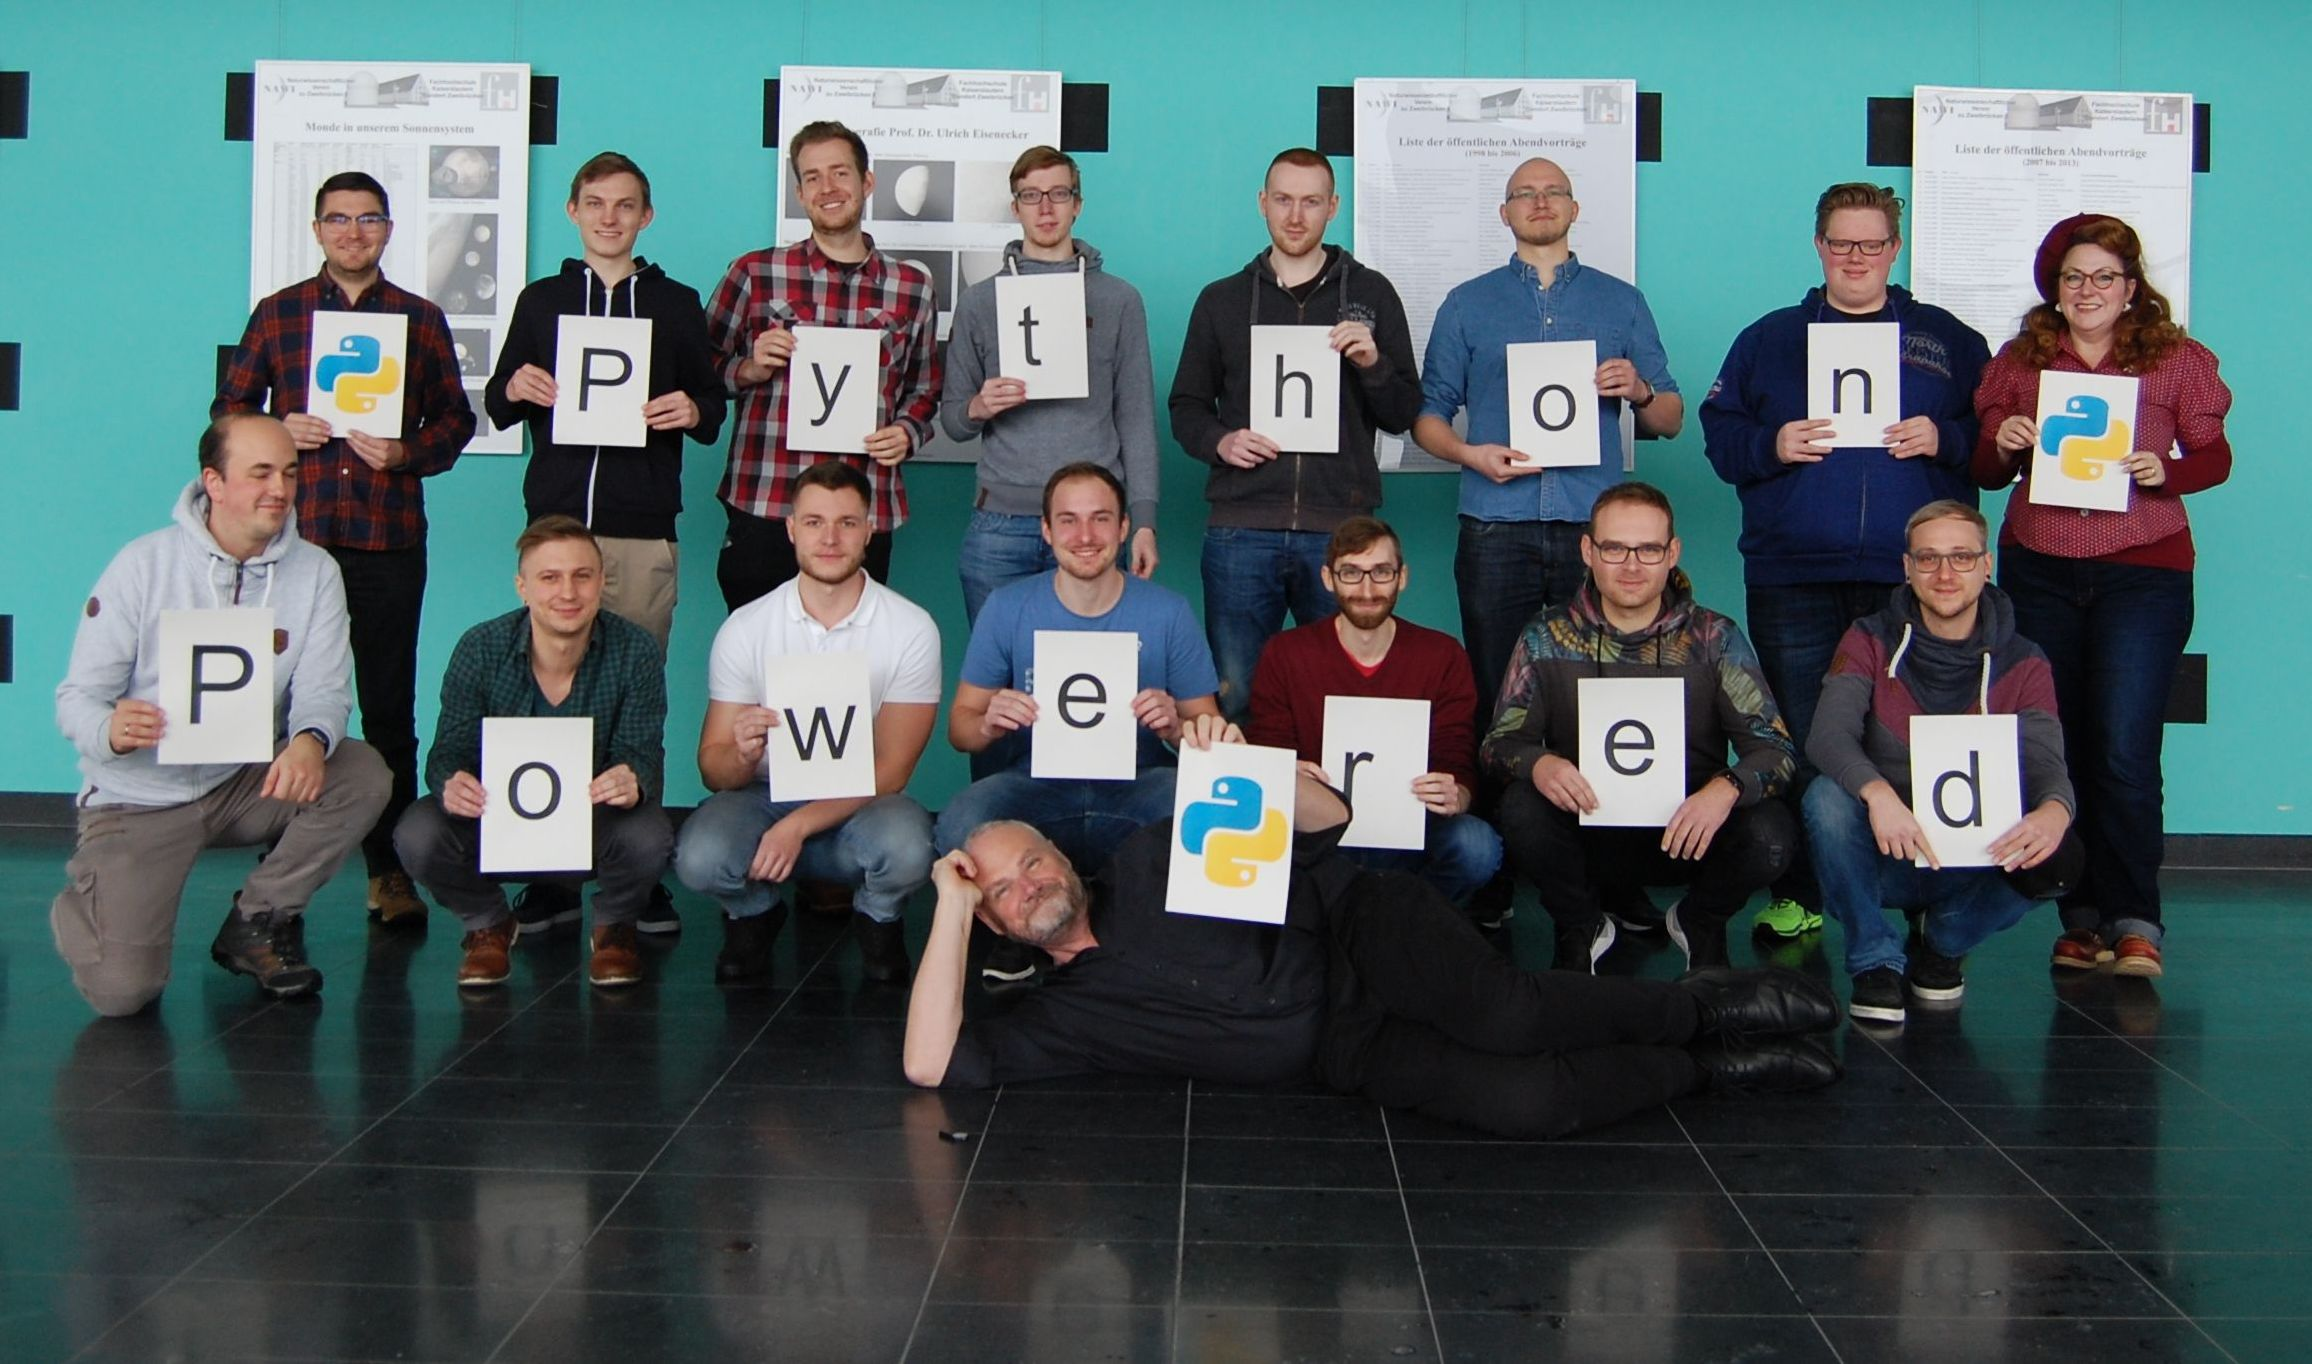
\includegraphics[width=\textwidth]{images/authors/theTeam}% Rotieren mit rotate=90
%\caption{\label{vorwort:team}Das Projektteam}
\end{figure}
\begin{tabular}{ll}
\centering
&Das Projektteam nach dem letzten Sprint Meeting\\
& im Januar 2019 von links nach rechts:\\
Hintere Reihe&Fabian Kalweit, Matthias Haselmaier, Marc Zintel,\\
                   &Robin Guth, Anatoli Sch�fer, Denis Schlusche,\\
                   &Kevin Konrad, Miriam Lohm�ller \\
Vordere Reihe&Mathias Fedder, Rainer Haffner, Lukas Kuhn,\\
                   &Sebastian Morsch, Julian Bernhart, Phillip Lauer,\\
                   &Christoph Seibel\\
Ganz vorne&Manfred Brill
\end{tabular}

\pagebreak
\subsection*{Die studentischen Autoren}
\begin{center}
\begin{tabular}{p{5cm}|l}
Julian  Bernhart&
\includegraphics[width=3cm]{images/authors/bernhart}\\
Eric Brunk&
\includegraphics[width=3cm]{images/authors/brunk}\\
Mathias Fedder&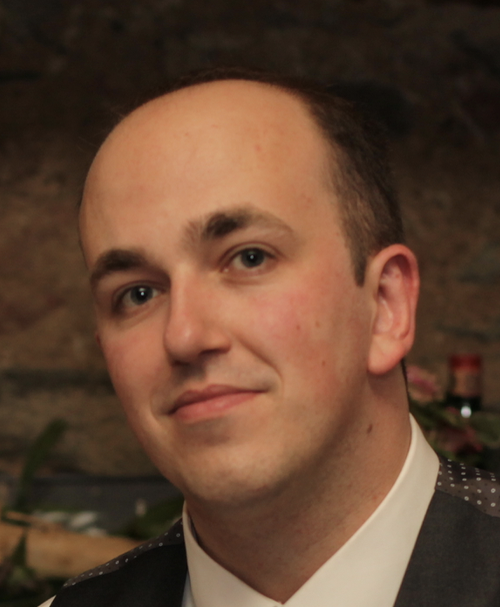
\includegraphics[width=3cm]{images/authors/fedder}\\
Christopher Gross&\\
Robin Guth&\\
Rainer Haffner&
\includegraphics[width=3cm]{images/authors/haffner}\\
Matthias Haselmaier&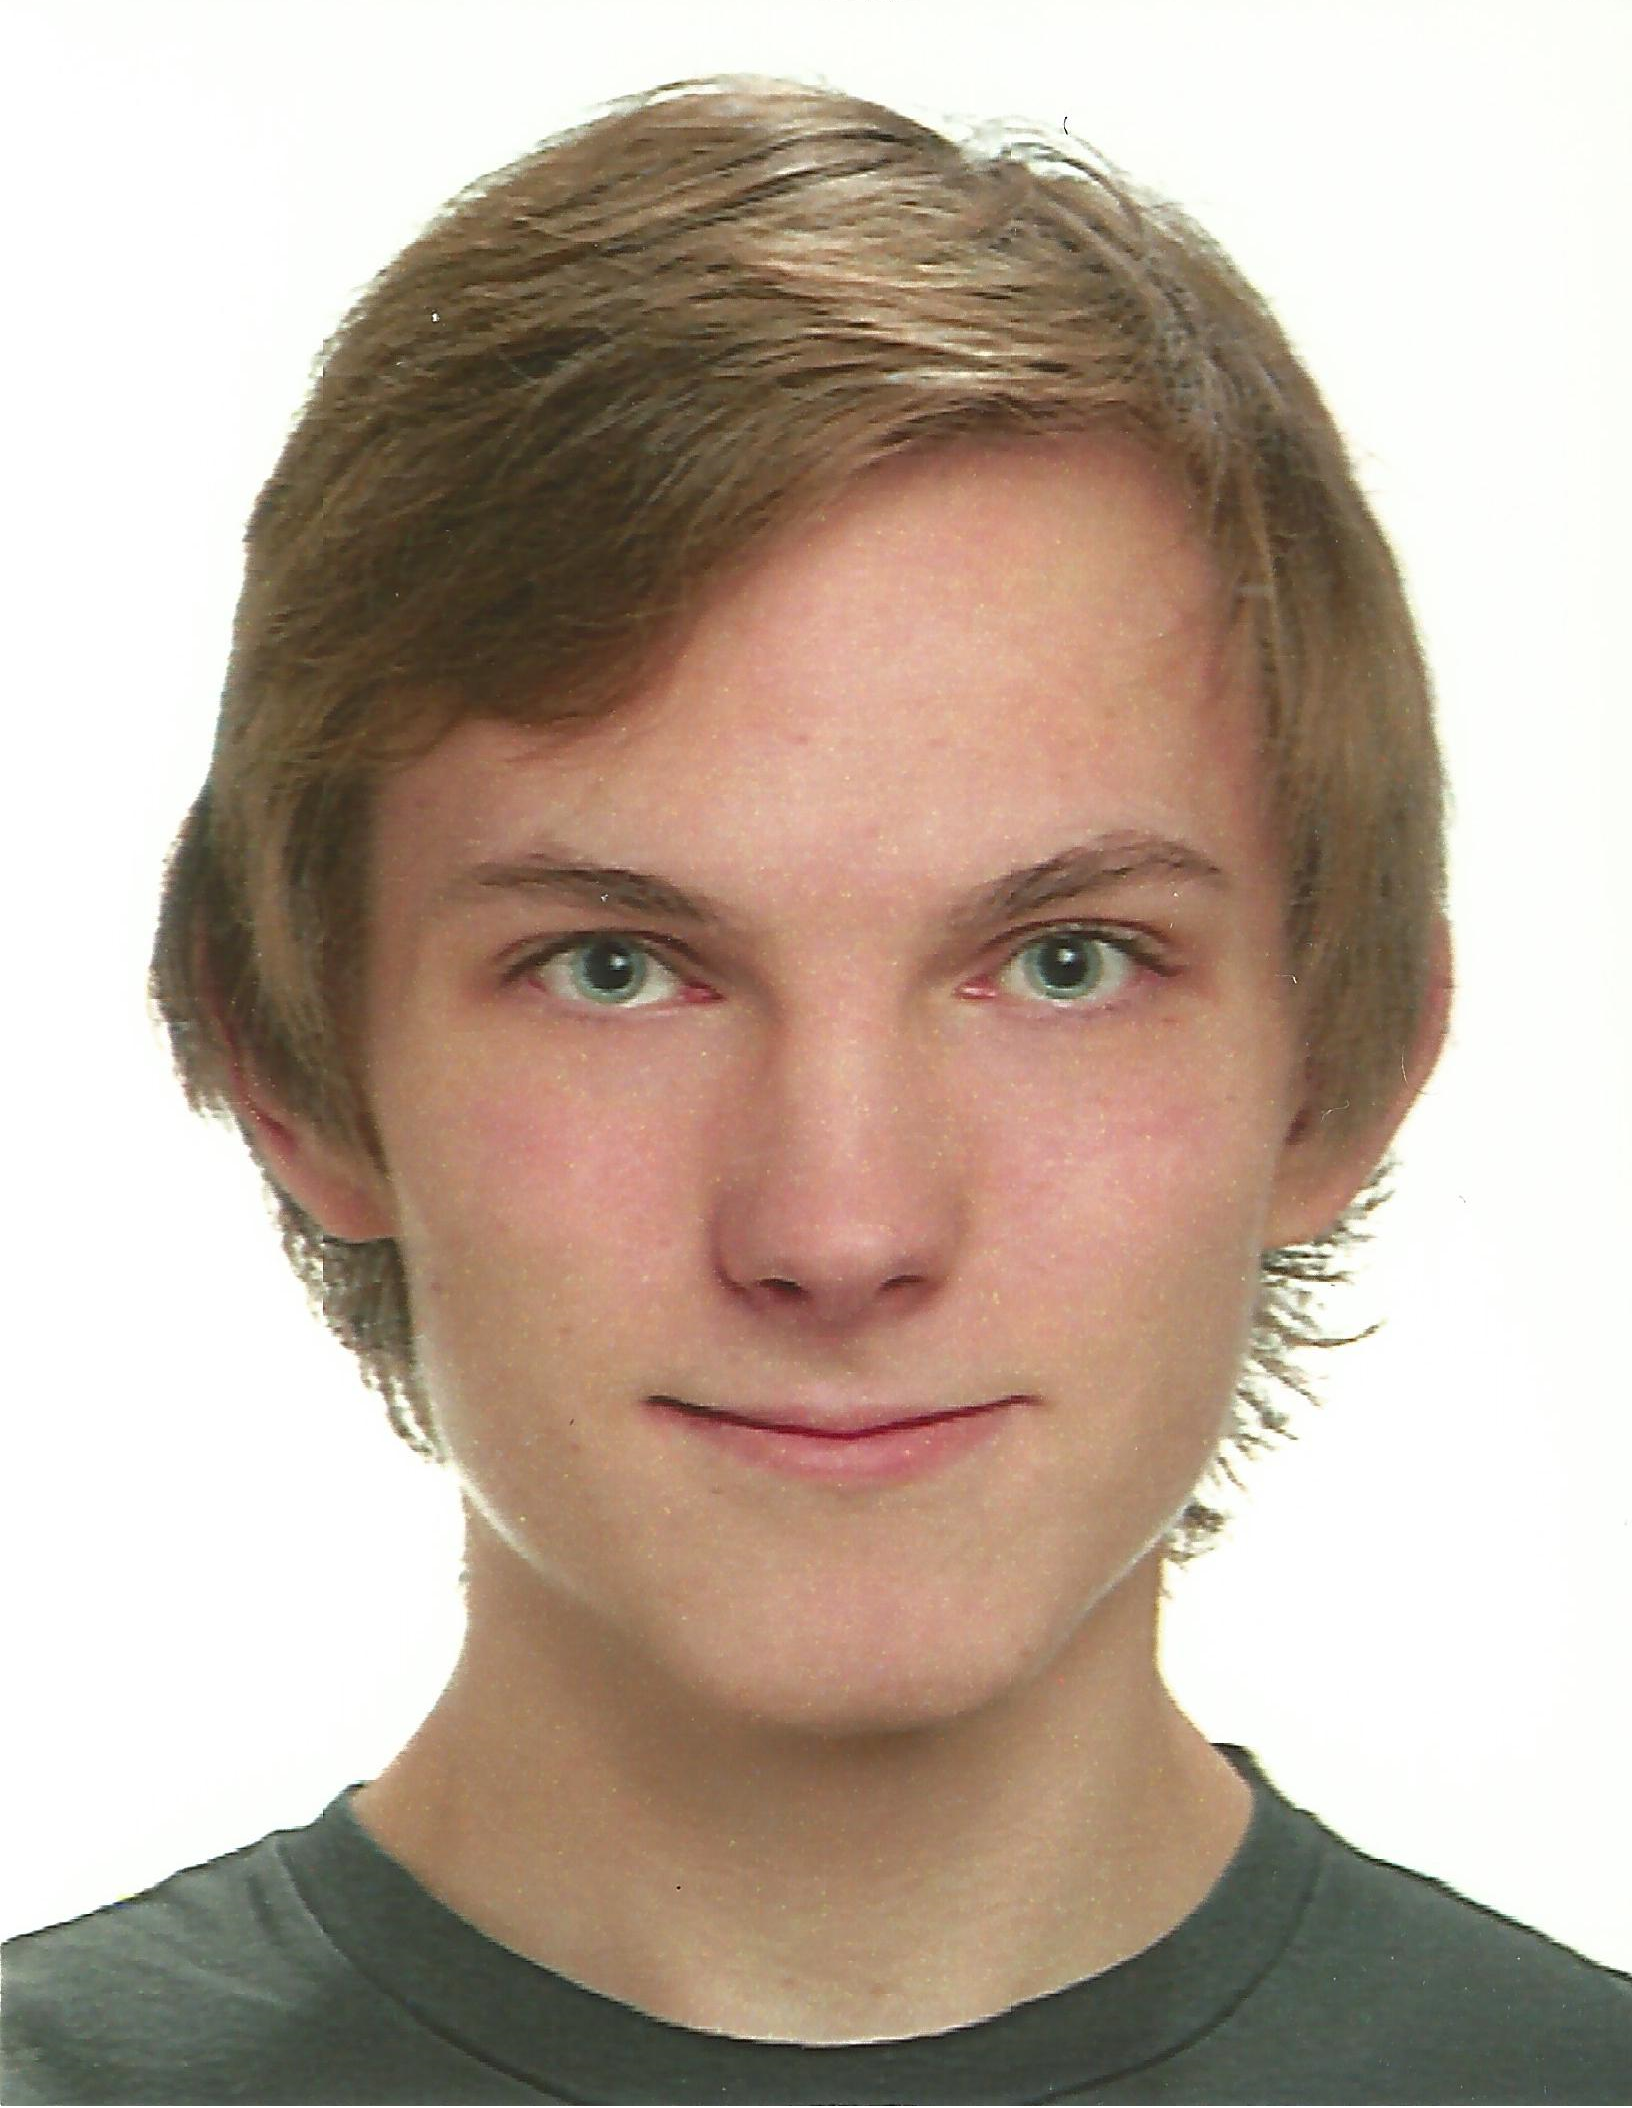
\includegraphics[width=3cm]{images/authors/haselmaier}\\
Kevin Konrad&\\
Lukas Kuhn&
\end{tabular}
\end{center}
\pagebreak
\begin{center}
\begin{tabular}{p{5cm}|l}
Philipp Lauer&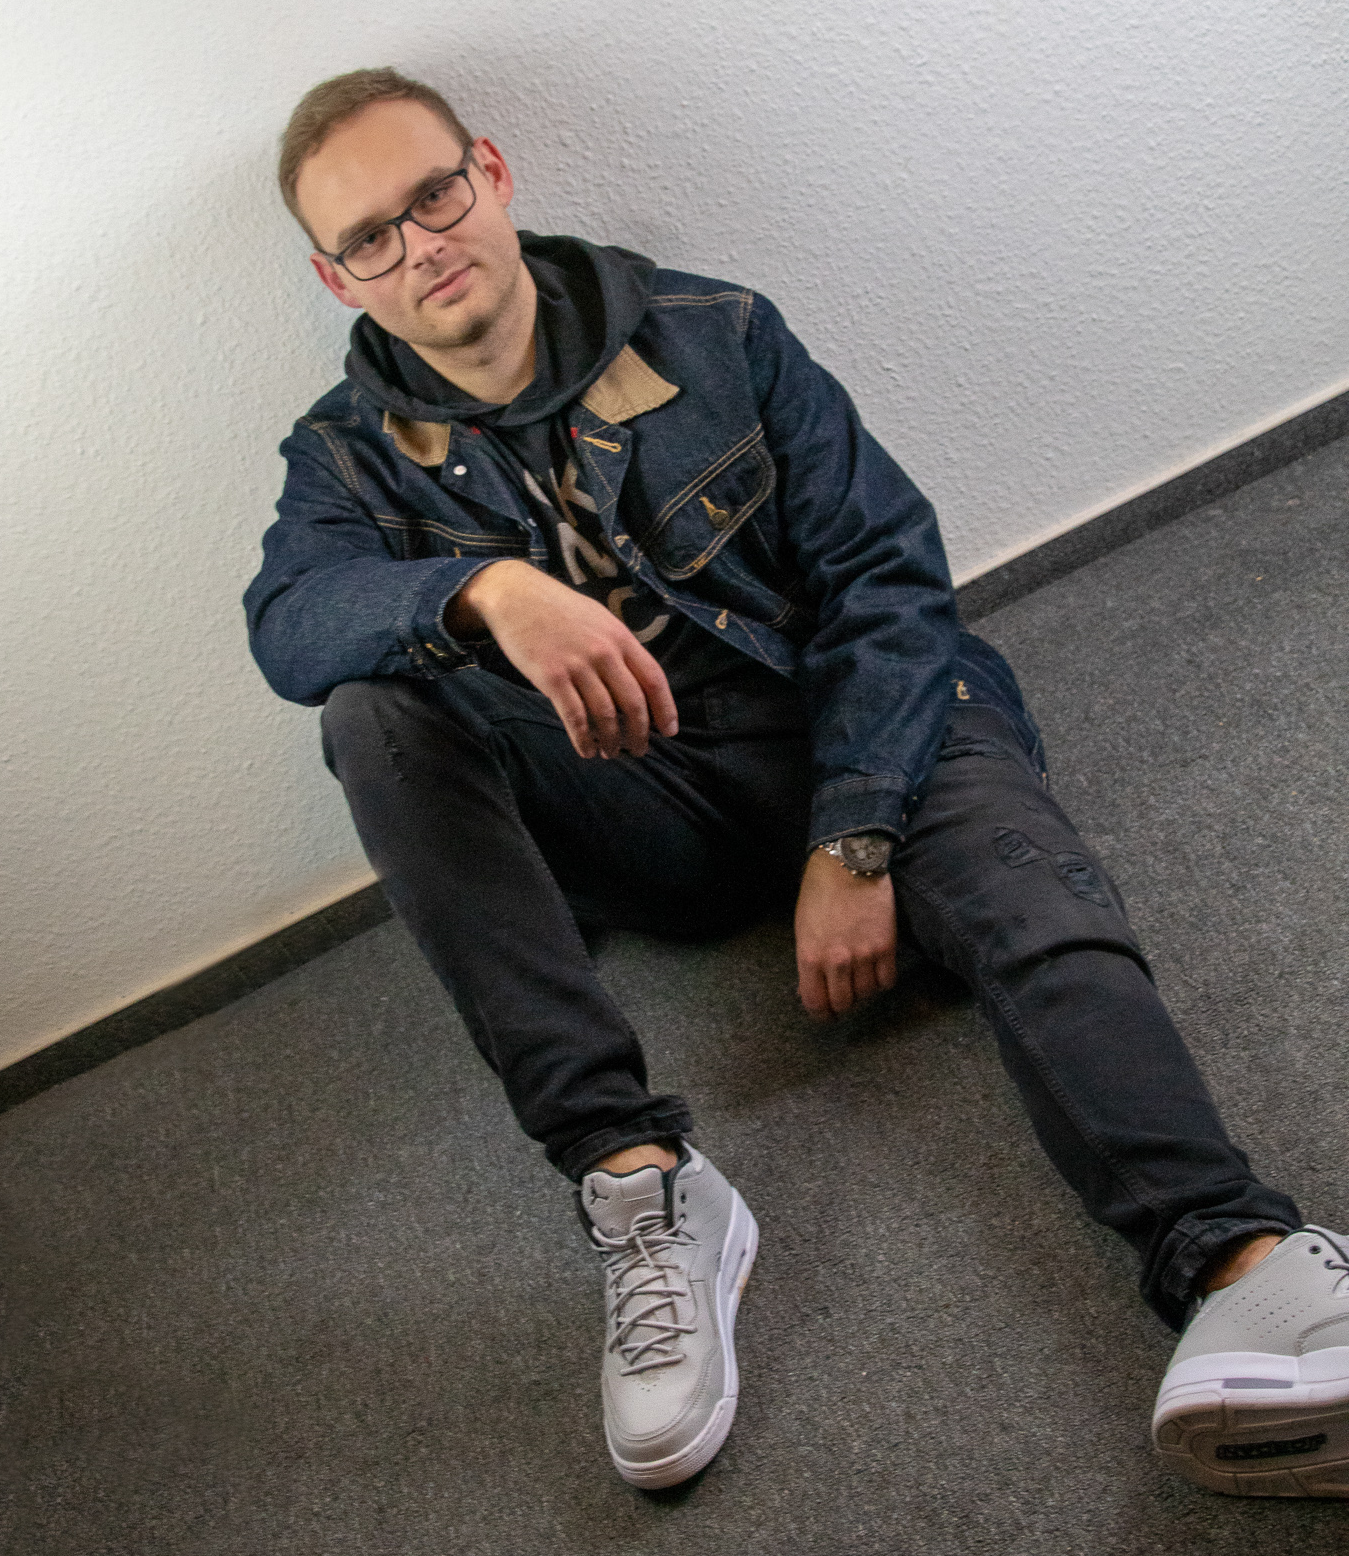
\includegraphics[width=3cm]{images/authors/lauer}\\
Sebastian Morsch&\\
Anatoli Sch�fer&\\
Denis Schlusche&\\
Christoph Seibel&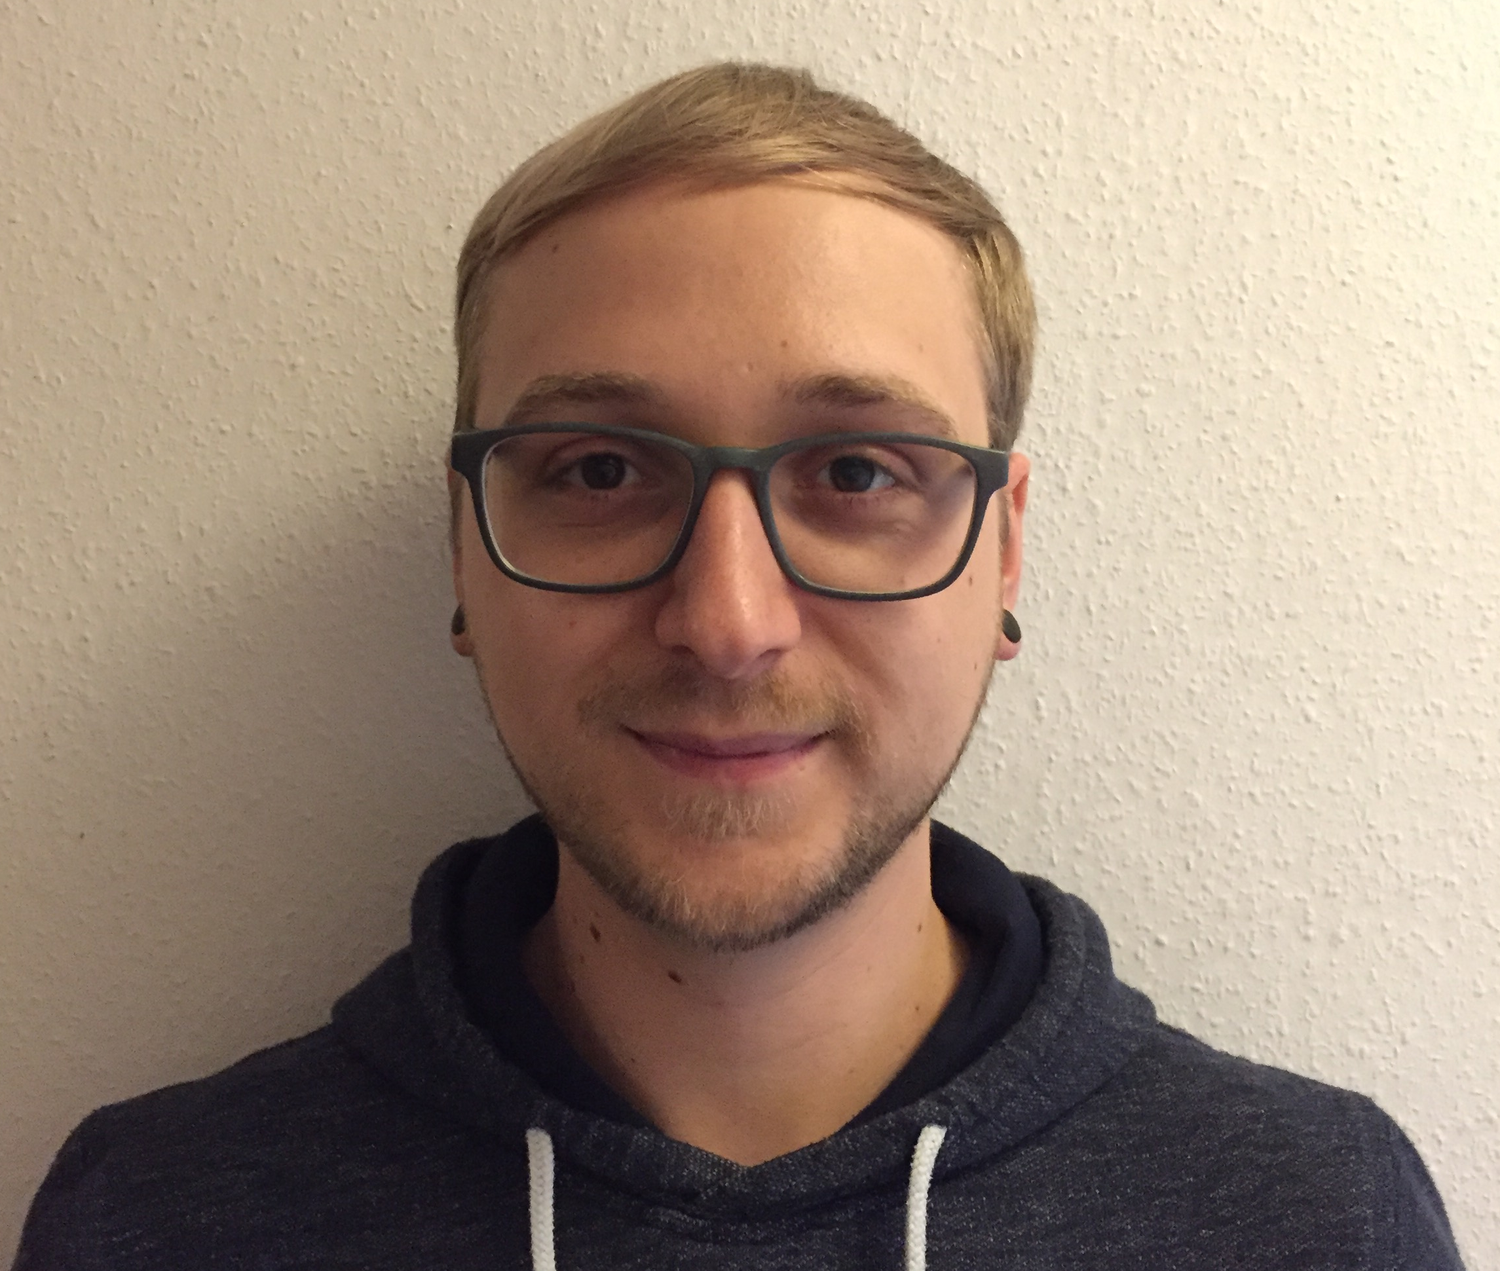
\includegraphics[width=3cm]{images/authors/seibel}\\
Marc Zintel&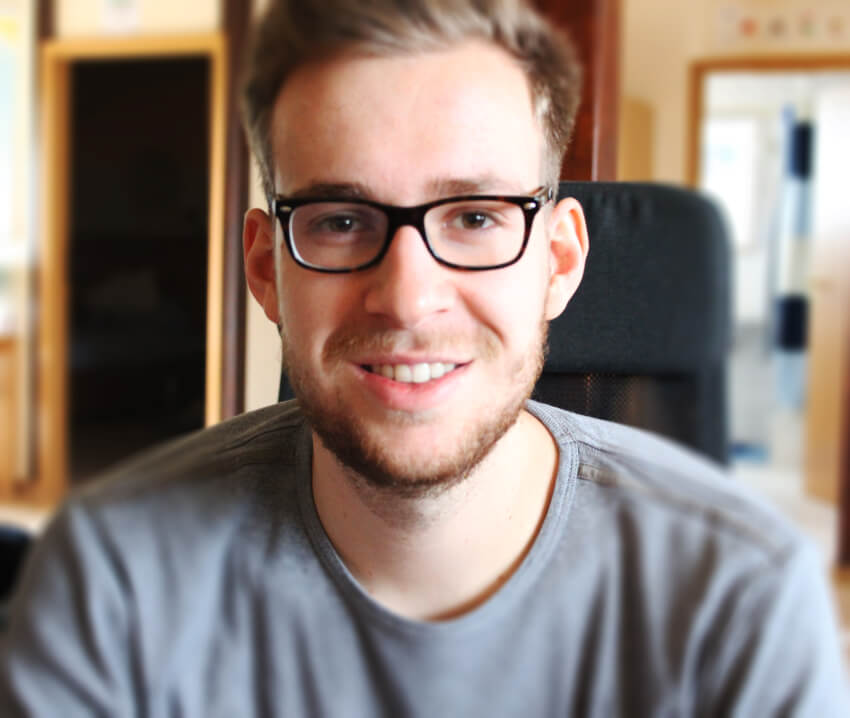
\includegraphics[width=3cm]{images/authors/zintel}
\end{tabular}
\end{center} 
%
% Inhaltsverzeichnis
%
\tableofcontents
\clearevenpage
\pagenumbering{arabic}
%
%
%
% !TeX root = ../../pythonTutorial.tex
\section{Was ist Python?}
\label{grundlagen:sec:WasIstPython}
Die Programmiersprache Python wurde Anfang der 1990er Jahre von Guido van Rossum als Universalprogrammiersprache entwickelt.
Der Name der Sprache beruht auf der Komikergruppe Monty Python.
Hierzu lassen sich auch zahlreiche Anspielung in der Dokumentation von Python finden.
Python wurde mit dem Ziel entworfen, eine einfache, gut verst�ndliche und �bersichtliche Programmiersprache zur Verf�gung zu stellen.
Dies soll nicht nur durch eine �bersichtliche Standardbibliothek erreicht werden, sondern auch durch die Modulare Erweiterbarkeit.
Im Folgenden wird die Programmiersprache Python in der Version 3 behandelt.

\section{Installation}

\label{grundlagen:sec:Installation}
Python \randnotiz{Installation} kann auf der Webseite \url{https://www.python.org} f�r eine Vielzahl von Betriebssystemen bezogen werden. 
Es stehen 32- und 64-Bit Versionen zur Verf�gung. 
Nach dem Start des Installationsassistenten wird der Nutzer durch die Installation gef�hrt. 
Der Ablauf der Installation unterscheidet sich je nach Betriebssystemen nur gering bis gar nicht.
Nach erfolgreichem Abschluss stehen dem Anwender verschiedene Programme f�r die Arbeit mit Python zur Verf�gung.
Im vom Nutzer gew�hlten Installationsverzeichnis befinden sich nun folgende Programme: 
\begin{description}
	\item[\textit{IDLE}] Standard IDE\footnote{Integrated Development Environment} f�r Python
	\item[\textit{Python}] Standard Konsolen Interpreter
	\item[\textit{Pythonw}] Standard Interpreter ohne Konsolenausgabe
\end{description}
Diese Programme reichen aus, um Code mit Python zu entwickeln. 
Der Python Interpreter kann in der Konsole mit dem Befehl \lstinline{python} aufgerufen werden. 
Die folgenden Abschnitte beschreiben Besonderheiten bei der Installation auf einzelnen Betriebssystemen. 
\subsection{Hinweis zur Installation unter Windows}
\label{grundlagen:sec:InstallationWindows}
Windows Nutzer m�ssen die Systemvariable f�r Python im Installationsassistenten hinzuf�gen lassen. 
Andernfalls kann Python nur im Installationsverzeichnis bzw. durch die Angabe des kompletten Pfads aufgerufen werden. 
In Abbildung \ref{grundlagen:img:InstallationWindows} ist die notwendige Auswahl zu sehen. 
\begin{figure}[ht]
	\centering
	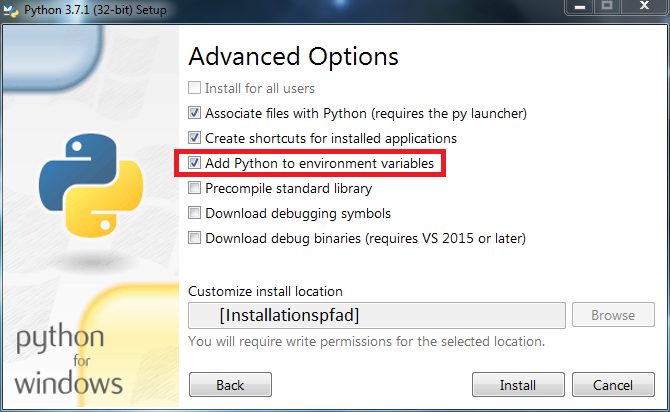
\includegraphics[scale=0.5]{images/InstallationWindows.png}
	\caption{Start des Installationsassistenten}
	\label{grundlagen:img:InstallationWindows}
\end{figure}
%
\subsection{Hinweis zur Installation unter Mac}
\label{grundlagen:sec:InstallationMac}
Im Folgenden wird die Installation unter macOS X gezeigt.

\begin{figure}[ht]
	\centering
	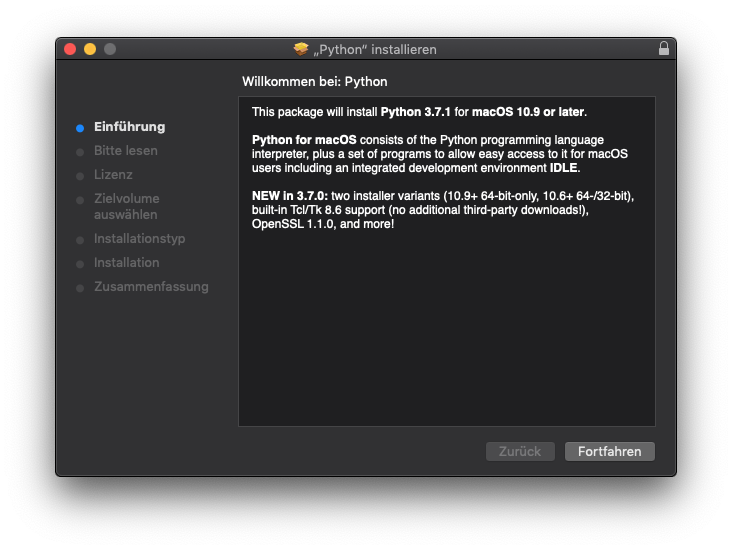
\includegraphics[scale=0.5]{images/InstallationMac.png} 
	\caption{Start des Installationsassistenten}
	\label{grundlagen:img:InstallationMac}
\end{figure}
Nach Ende der Installation befindet sich der Python Ordner im Finder (Dateiexplorer).

\begin{figure}[ht]
	\centering
	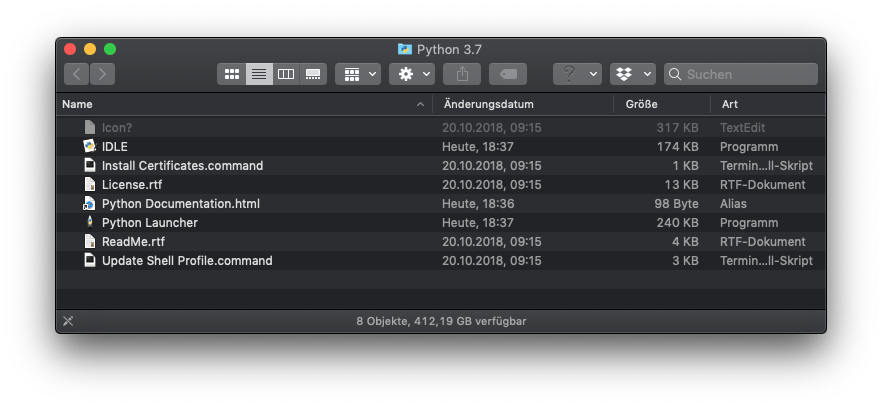
\includegraphics[scale=0.5]{images/PythonFinder.png} 
	\caption{Fertige Installation}
	\label{grundlagen:img:FinishInstall}
\end{figure}
Zuletzt wurde durch den Assistent unter \texttt{/Library/Frameworks/\\Python.framework} noch das Python Framework abgelegt.
Ohne das w�re die Arbeit mit Python unter Mac nicht m�glich.

\subsection{Hinweis zur Installation unter Linux(Ubuntu)}
\label{grundlagen:sec:InstallationLinux}
In diesem Kapitel wird die Installation f�r Ubuntu Version 18.04.1 LTS erl�utert.
Im Gegensatz zu den anderen Betriebssystemen, wird hier nur der Python Interpreter in der Version 3.6.6 mitgeliefert
Standard Entwicklungsumgebung IDLE ist nicht vorinstalliert.
Diese kann �ber das Paket IDLE nachtr�glich installiert werden.
Sollte die Arbeit mit Python noch nicht m�glich sein, kann durch den folgenden Befehl die Installation manuell angesto�en werden.

\begin{lstlisting}[language=BASH, label={grundlagen:lst:InstallationLinux}]
sudo apt-get install python3 python-doc
\end{lstlisting}

Diese Installation umfasst unter anderem auch die Dokumentation von Python.
Nach Abschluss der Installationsroutine kann wie mit jedem anderen Betriebssystem mit Python gearbeitet werden.

\section{Python Interpreter} 
\label{grundlagen:sec:Interpreter}
Die einfachste M�glichkeit, Python Code auszuf�hren, ist die direkte �bergabe des Codes an den sogenannten Python Interpreter. 
Dabei handelt es sich um eine Konsolenanwendung, die Code ausf�hren und gegebenenfalls auftretende Ergebnisse ausgeben kann. 
Dabei kann ein Nutzer den Code entweder direkt in die Konsole eingeben oder aus einer Datei auslesen lassen. 
Wie bei anderen Programmiersprachen auch, stehen f�r Python verschiedene IDEs zur Verf�gung, welche in Kapitel \ref{ides:section:ides} behandelt werden. 
F�r die ersten Versuche mit Python reicht der Interpreter jedoch v�llig aus. Dieser wird standardm��ig mit Python installiert.

In Abbildung \ref{grundlagen:img:Interpreter} ist der Interpreter zu sehen. 
Zus�tzlich zur Version werden auch noch der Herausgeber von Python sowie die Uhrzeit angezeigt.
Bereits jetzt kann erster Code ausgef�hrt werden.
Im Folgenden werden zu einzelnen Bestandteilen von Python Beispiele beigef�gt, die leicht im Interpreter ausf�hrbar sind. 
Es wird dem Leser empfohlen, sie zum besseren Verst�ndnis nachzuvollziehen, falls m�glich durch selbst�ndiges Ausprobieren.

\begin{figure}[ht]
	\centering
	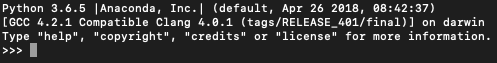
\includegraphics[width=0.8\textwidth]{images/Interpreter.png} 
	\caption{Ansicht nach Start des Interpreters}
	\label{grundlagen:img:Interpreter}
\end{figure}

\subsection*{Interaktiver Modus} 
\label{grundlagen:sec:InteraktiverModus}
Wird der Interpreter ohne Angabe einer Quellcodedatei gestartet, befindet dieser sich im interaktiven Modus. 
Der Nutzer kann hier direkt Anweisungen eingeben. Durch die Ausgabe der Zeichen $>>>$ zeigt die Konsole an, dass sie eine Anweisung erwartet. 
In Python existieren auch mehrzeilige Anweisungen. 
Nach der Eingabe der ersten Zeile werden die Zeichen $...$ ausgegeben, was bedeutet, dass Folgeanweisungen erwartet werden. 
\subsection*{Einlesen einer Datei}
\label{grundlagen:sec:EinlesenDatei}
Auf Dauer ist die direkte �bergabe des Codes an den Interpreter sehr unpraktisch. 
Um Code erneut nutzen zu k�nnen und zu speichern, kann dieser in Dateien abgelegt werden.
Dies kann mit einem simplen Texteditor erfolgen.
Dateien, die Python Code enthalten, werden mit der Dateiendung ''.py'' gekennzeichnet. 
Sie k�nnen direkt mit dem der Konsole ausgef�hrt werden.
Dazu muss Python der relative Pfad der Pythondatei (.py-Endung) �bergeben werden.  
\begin{lstlisting}[language=BASH, label={grundlagen:lst:BashStartPython1}]
python <Relativer Dateipfad der Pythondatei>
\end{lstlisting} 
Da nur der relative Pfad angegeben werden muss, muss lediglich der Dateiname angegeben werden, falls die Konsole sich bereits im selben Verzeichnis wie die zu �ffnende Datei befindet.
\section{Syntax}
\label{grundlagen:sec:Syntax}
Im \randnotiz{Syntax} Folgenden werden wichtige Grundkonzepte der Programmiersprache\\ \mbox{Python} erl�utert.
%Benoetigt um korrekten Zeilenumbruch zu erzwingen
\subsection{Allgemeine Strukturen}
\label{grundlagen:sec:AllgemeineStrukturen}
Anders als bei anderen Programmiersprachen wie beispielsweise Java oder C++, ben�tigt Python keine Klassenkonstrukte oder main-Methoden zur Ausf�hrung. 
Das bedeutet, dass einzelne Anweisungen in Python korrekt ausgef�hrt werden k�nnen. 
Sollten f�r die Bearbeitung von komplexeren Problemen objektorientierte Ans�tze ben�tigt werden, kann auch dies mit Python umgesetzt werden. 
Weitere Informationen zur Objektorientierung mit Python finden sich im weiteren Verlauf des Python Tutorials.
F�r den Moment reicht es f�r den Leser zu wissen, dass Anweisungen bereits zeilenweise ausgef�hrt werden k�nnen. 
Das kann sehr simpel getestet werden, indem der Python Interpreter als einfacher Taschenrechner genutzt wird. 
In Abbildung \ref{grundlagen:img:AusdrueckeInInterpreter} wird dies gezeigt. Einfache Ausdr�cke wie Summen, Subtraktionen, Multiplikationen und Divisionen k�nnen direkt eingegeben werden. 
Nach Bet�tigung der Eingabe-Taste liefert Python das Ergebnis des Ausdrucks.\\
\begin{figure}
	\centering
	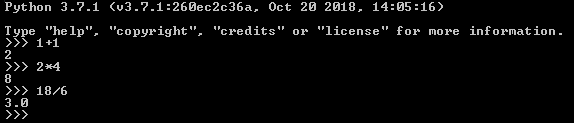
\includegraphics[width=1\textwidth]{images/AusdrueckeInInterpreter.png} 
	\caption{Einfache Ausdr�cke im Python Interpreter}
	\label{grundlagen:img:AusdrueckeInInterpreter}
\end{figure}
\subsection{Leerzeichen und Einr�ckung}
\label{grundlagen:sec:LeerzeichenEinrueckung}
Um in Python Bl�cke auszuzeichnen, werden im Gegensatz zu Java oder C++ keine geschweiften Klammern genutzt.
In Python werden Bl�cke durch das Einr�cken der Zeilen markiert. 
Hierf�r sind entweder der Tabulator oder vier aufeinander folgende Leerzeichen vorgesehen.
\subsection{Kommentare}
\label{grundlagen:sec:Kommentare}
Innerhalb der Programmiersprache Python wird zwischen Zeilen- und Blockkommentaren unterschieden.
Zeilenweise Kommentare werden durch das Rautensymbol \lstinline$\#$ eingeleitet.
Blockkommentare hingegen werden durch drei aufeinander folgende Anf�hrungszeichen \lstinline$"""$ jeweils zu Beginn und am Ende des Kommentars markiert.
Hier wird jeweils ein Beispiel gezeigt:

\lstinputlisting[language=Python,label={grundlagen:lst:Kommentare}]{chapters/basics/src/comment.py}
\subsection{Typsicherheit}
\label{grundlagen:sec:Typsicherheit}
Anders als bei Java und C++ ist Python eine nur schwach typisierte Sprache.
Somit ist bei der Initialisierung keine Typangabe erforderlich.
Der Datentyp wird beim Initialisieren dynamisch ermittelt und automatisch zugewiesen.
Um einer Variable trotzdem einen gew�nschten Typ zuzuweisen, kann man sie einfach mit dem entsprechenden Typ initialisieren.
Weitere Informationen zu Datentypen werden in Abschnitt \ref{basicdatatypes:sec:ElementareDatentypen} erl�utert.
\section{Beispiel \glqq Hello World!\grqq}
\label{grundlagen:sec:HalloWorld}
Einfache \randnotiz{Beispiel} Ausgaben k�nnen mit der print()- Anweisung gemacht werden. 
Innerhalb der Klammern muss ein String �bergeben werden, sprich eine einfache Zeichenkette. 
Diese wird durch umschlie�ende einfache oder doppelte Anf�hrungszeichen markiert (''EinString''/'EinString'). 
Der Einfachheit halber, wird hier noch auf die genaue Erkl�rung der einzelnen Bestandteile der Anweisung verzichtet. 
Ein einfaches ''Hello-World!''-Programm ben�tigt in Python nur eine Zeile: 
\lstinputlisting[language=python, label={grundlagen:lst:HalloWorld}]{chapters/basics/src/helloworld.py} 
Es handelt sich dabei um ein vollst�ndiges Python-Programm, das in dieser Form ausgef�hrt werden kann. 
Wie bereits erl�utert, werden anders als bei Java oder C++ keine Klassenkonstrukte oder main-Methoden ben�tigt.

%\uebung
%\aufgabe{grundlagen01} 
%\aufgabe{grundlagen02}

\uebungTutorial{grundlagen01}{grundlagen02}


% !TeX root = ../pythonTutorial.tex
\chapter{Ein- und Ausgabe}
\label{chapter:inputoutput}

In Python gibt es verschiedene Methoden, um Daten vom Benutzer entgegenzunehmen und Daten dem Benutzer zur Verf�gung zustellen.

% !TeX root = ../../pythonTutorial.tex
\section{Konsolenausgabe mit print()}
\label{printInOut}

Die \emph{print()}-Funktion hat vielerlei Nutzen und wird entsprechend oft verwendet. Daher ist es definitiv sinnvoll, sich mit ihr vertraut zu machen.

\begin{lstlisting}[language=Python, label=printInOut:lst:printDefault]
# die Print-Methode

print(value1, value2, ..., sep=" ", 
    end="\n", file=sys.stdout, flush= false))
\end{lstlisting}

In Listing (\ref{printInOut:lst:printDefault}) sind die Parameter von \lstinline$print()$ zu sehen. Die auszugebenden Werte stehen an erster Stelle (value1, value2, ...), hierbei handelt es sich um eine beliebige Anzahl an Werten. Der Parameter \lstinline$sep$ bildet den Seperator zwischen den Werten und hat als Standardwert das Leerzeichen.
\randnotiz{Seperator}
In Listing \ref{printInOut:lst:printSeperator} k�nnen wir sehen, dass wir durch Angabe eines Seperators eine bessere Lesbarkeit erreichen k�nnen.

\begin{lstlisting}[language=Python, label=printInOut:lst:printSeperator]
# die Print-Methode mit Seperator

print(1,2,3)
# Ausgabe: 1 2 3

print(1,2,3, sep=" | ")
# Ausgabe: 1 | 2 | 3
\end{lstlisting}

Nach dem Seperator folgt der \emph{end}-Parameter, dieser f�gt standardgem�� einen Zeilenumbruch (\textbackslash n) an das Ende der Ausgabe.
\randnotiz{End-Angabe}

\begin{lstlisting}[language=Python, label=printInOut:lst:printEnd]
# die Print-Methode mit End-Angabe

print("Satz mit Zeilenumbruch")
print("N�chster Satz")
# Ausgabe:
# Satz mit Zeilenumbruch
# N�chster Satz

print("Satz mit Punkt und Leerzeichen." , end=". ")
print("N�chster Satz)
# Ausgabe: 
# Satz mit Punkt und Leerzeichen. N�chster Satz
\end{lstlisting}

Der \emph{file}-Parameter bestimmt den Datenstrom (\emph{Stream}) f�r den Output. In \lstinline$sys.stdout$ steht f�r die Konsole. 
\randnotiz{Output-Stream}
M�chten wir den Output bspw. in eine Textdatei schreiben, dann k�nnen wir diese als Ziel des Datenstroms festlegen.

\begin{lstlisting}[language=Python, label=printInOut:lst:printFile]
# die Print-Methode mit Ausgabe in Textdatei

# open() -> festlegen einer Textdatei als Stream
# "w" steht f�r 'write' und gibt an,
# dass wir etwas in die Datei schreiben m�chten

txtFile = open(beispielText.txt, "w")
print("Hello, World.", file="txtFile")
txtFile.close()
# close() schlie�t den Stream
\end{lstlisting}

\kontrollfrage{
	\item[\kontroll] Was sind die Parameter der \lstinline$print()$-Funktion?
	\item[\kontroll] Welche Funktionalit�t bietet uns die \lstinline$print($)-Funktion?
	\item[\kontroll] Was ist der Unterschied zwischen dem Seperator und dem \lstinline{end}-Parameter?
}


% !TeX root = ../../pythonTutorial.tex
\section{Formatierung von Strings}
\label{formatInOut}

Es w�re sicherlich hilfreich, wenn wir die String-Ausgaben nach belieben formatieren k�nnten. Bisher haben wir den Seperator von \lstinline$print()$ kennengelernt - dieser ist von seiner Funktionsweise jedoch stark beschr�nkt. Python bietet uns hierf�r die \lstinline$format()$-Methode an, vorher betrachten wir aber die Modulo-Arithmetik und machen uns mit den Formatierungszeichen vertraut.

Mittels Modulo-Arithmetik \randnotiz{Modulo-
Arithmetik} leiten wir ein Formatierungszeichen ein. Dieses gilt als Platzhalter f�r einen Wert.

\begin{lstlisting}[language=Python, label=formatInOut:lst:modulo]
# Modulo-Arithmetik

print("K�rper: %s , Fl�che: %f" %
    ('Dreieck', 42.6))

# Ausgabe:
# K�rper: Dreieck , Fl�che: 42.6
\end{lstlisting}

Bei "'K�rper"' setzen wir den ersten Platzhalter mit "'\%s"'. Die Reihenfolge der Platzhalter setzt fest, welcher Wert anschlie�end eingebunden wird. Der erste Platzhalter tr�gt also den ersten Wert, der nach dem Ausgabetext folgt, der zweite den zweiten und so weiter.

\warning{Die einzusetzenden Werte werden nach dem String mittels Modulo als Tupel festgelegt!}

Das Formatierungszeichen nach dem Modulo bestimmt den Datentyp des Wertes.
Bei "'s"' handelt es sich um einen String, bei "'f"' um ein \emph{float}.
In Tabelle \ref{formatInOut:fig:formatierungszeichen} sind die m�glichen Formatierungszeichen aufgelistet.

\begin{table}[ht]
\centering
\caption{\label{formatInOut:fig:formatierungszeichen}Formatierungszeichen und ihre Bedeutung (\cite{klein2018})}
\small
\begin{tabular}{l|l}\hline
Platzhaltersymbol&Bedeutung\\\hline
\lstinline$d$&Vorzeichenbehaftete Ganzzahl (Integer, dezimal)\\
\lstinline$i$&Vorzeichenbehaftete Ganzzahl (Integer, dezimal)\\
\lstinline$o$&vorzeichenlose Ganzzahlen (oktal)\\
\lstinline$u$&vorzeichenlose Ganzzahlen (dezimal)\\
\lstinline$x$&vorzeichenlose Ganzzahlen (hexadezimal)\\
\lstinline$X$&vorzeichenlose Ganzzahlen (hexadezimal)\\
\lstinline$e$&Flie�kommazahl im Exponentialformal\\
\lstinline$E$&Flie�kommazahl im Exponentialformat\\
\lstinline$f$&wie \lstinline$e$\\
\lstinline$F$&wie \lstinline$E$\\
\lstinline$g$&Wie \lstinline$e$, wenn der Exponent gr��er ist als $-4$\\
           &oder kleiner als die Pr�zision. Ansonsten wie \lstinline$f$\\
\lstinline$G$&wie \lstinline$E$ und analog zu \lstinline$g$\\
\lstinline$c$&ein Zeichen\\
\lstinline$s$&Eine Zeichenkette (String), beliebige Python-Objekte\\
                 &werden in String mittel der Methode \lstinline$str()$ gewandelt.\\
\lstinline$r$&wie \lstinline$s$\\
\lstinline$%$&Es findet keine Konvertierung des Arguments statt,\\
     &es wird ein \lstinline$%$-Zeichen ausgegeben\\\hline
\end{tabular}
\end{table}

\kontrollfrage{
    \item[\kontroll] Wir errichten einen Platzhalter \%d und geben den einzusetzenden Wert '2.3' an. Ausgegeben wird der Wert '2', wieso?
    \item[\kontroll] Wie bestimmen wir, welcher Wert zu welchem Platzhalter geh�rt?}

Was ist jedoch, falls die Ausgabe eine bestimmte L�nge haben soll?
Mit Hilfe der Syntax der Modulo-Arithmetik k�nnen wir dieses Problem l�sen.

 \begin{lstlisting}[language=Python, label=formatInOut:lst:syntax]
 # Modulo-Arithmetik Syntax

%[Flag][Minimum der Gesamtl�nge].[Pr�zision][Typ]
 \end{lstlisting}

 Das Minimum der Gesamtl�nge bringt gro�e Vorteile mit sich, wenn wir z.B. einen linksb�ndigen Text ausgeben wollen. Alle Ausgaben, die k�rzer als das vorgegebene Minimum sind, werden mit Leerzeichen aufgef�llt.

 \warning{Es handelt sich hierbei um das Minimum der Gesamtl�nge. Alle Ausgaben die gr��er sind, werden nicht beschr�nkt und in voller L�nge ausgegeben!}

 Mittels Punkt k�nnen wir folgend die Pr�zision einstellen, was bei einem \lstinline$Float$-Datentyp die Nachkommastellen bestimmt. Alle Zahlen werden zu der angegebenen Nachkommastelle aufgerundet!

 \begin{lstlisting}[language=Python, label=formatInOut:lst:precision]
 # Modulo-Arithmetik Pr�zision

print("Eine Zahl %f" % (1.234))
print("Eine gerundete Zahl %.2f)

# Ausgabe:
# Eine Zahl 1.234
# Eine gerundete Zahl 1.23
\end{lstlisting}

\subsection{Formatierung mit format()}

Python bietet uns f�r die Formatierung von String-Elementen die Methode \lstinline$format()$.

 \begin{lstlisting}[language=Python, label=formatInOut:lst:formatMethod]
# Syntax der format()-Methode

string.format(par0, par1, ..., key0=val0, key1=val1, ...)
\end{lstlisting}

\lstinline$format()$ ersetzt markierte Stellen im gegebenen String durch angegebene Werte (Parameter in \lstinline$format()$) und liefert diesen zur�ck.
Die Stellen werden durch geschweifte Klammern markiert und mittels Modulo-Arithmetik pr�zisiert. In der geschweiften Klammer geben wir als erstes den Index (oder das Schl�sselwort) des Parameters an.

 \begin{lstlisting}[language=Python, label=formatInOut:lst:formatString]
# format() mit gegebenem String

str = "Hallo, {0:s} und {1:s}"
print(str.format("Rainer", "Denis"))
# Ausgabe:
# Hallo, Rainer und Denis

print(str)
# Ausgabe:
# Hallo, {0:s} und {1:s}

# format() ver�ndert den String nicht,
# sondern liefert den ver�nderten Wert zur�ck

str = str.format("Rainer", "Denis")
print(str)
# Ausgabe:
# Hallo, Rainer und Denis

# der Wert von 'str' wurde durch den R�ckgabewert
# von format() �berschrieben!

str = "Hallo, {1:s} und {0:s}"
str.format("Rainer", "Denis")
print(str)
# Ausgabe:
# Hallo, Denis und Rainer

# in 'str' wurde der angegebene Index vertauscht

str = "Hallo, {r:s} und {d:s}"
print(str.format(r = "Rainer", d ="Denis"))
# Ausgabe:
# Hallo, Rainer und Denis

# Angabe von Schl�sselwort-Parametern
\end{lstlisting}

\warning{M�chte man geschweifte Klammern ausgeben, dann werden diese doppelt geschrieben ("'\{\{"' und "'\}\}"')}

Die \lstinline$format()$-Methode bietet uns au�erdem Ausrichtungsoptionen, was zu besserer Lesbarkeit beitragen kann. Somit k�nnen wir bspw. Werte links- oder rechtsb�ndig ausgeben. Hierf�r gibt man die Formatierungsanweisung wie in Tabelle \ref{formatInOut:leftRight} an und den Wert des Abstandes bzw. der Gr��e des Platzhalters. Ist das Wort zu kurz, wird der restliche Platz mit Leerzeichen aufgef�llt.

\begin{table}[h]
\centering
\caption{\label{formatInOut:leftRight}Links- und rechtsb�ndiger Text}
\begin{tabular}{|c | p{8cm}|}
    \hline
    Formatierungsanweisung & Bedeutung \\
    \hline
    < & Text wird linksb�ndig ausgelegt \\
    > & Text wird rechtsb�ndig ausgelegt \\
    \hline
\end{tabular}
\end{table}

\begin{lstlisting}[language=Python, label=formatInOut:lst:formatAlignment]
# Ausrichtung mit Formatierungsanweisung

# linksb�ndig
str = "{0:<10s} {1:d}"
print(str.format("Viereck", 4))
print(str.format("F�nfeck", 5))
print(str.format("Sechseck", 6))

# Ausgabe:
# Viereck    4
# F�nfeck    5
# Sechseck   6


# rechtsb�nding
str = "{0:>10s} {1:d}"
print(str.format("Viereck", 4))
print(str.format("F�nfeck", 5))
print(str.format("Sechseck", 6))

# Ausgabe:
#    Viereck 4
#    F�nfeck 5
#   Sechseck 6
\end{lstlisting}

Python bietet uns f�r \lstinline{Dictionaries} einen einfachen Weg, diese mittels \lstinline$format()$ und der Nutzung von Schl�sselwort-Parametern, auszugeben.

\begin{lstlisting}[language=Python, label=formatInOut:lst:formatDict]
# Formatierung eines Dictionarys

dictMath = {"Dreieck" : "3",
       "Viereck" : "4",
       "F�nfeck" : "5",

str = "{body}: {corners}"

for geoBody in dictMath
    print(str.format(body=geoBody,
                     corners=dictMath[geoBody]))

# Ausgabe:
# Dreieck: 3
# Viereck: 4
# F�nfeck: 5
\end{lstlisting}


% !TeX root = ../../pythonTutorial.tex
\section{Konsoleneingabe mit input()}
\label{inputInOut}

Mit Hilfe von \lstinline$input()$ erlauben wir dem Nutzer Eingaben �ber die Konsole. Somit erhalten wir den ersten Grad an Interaktion zwischen Nutzer und Programm.

\begin{lstlisting}[language=Python, label=inputInOut:lst:inputDefault]
# die input-Methode

input(prompt)
\end{lstlisting}

Sobald \lstinline$input()$ aufgerufen wird, wartet das Programm mit dem weiteren Ablauf, bis der Nutzer seine Eingabe mit der Eingabetaste best�tigt.
Die \lstinline$input()$-Methode liefert den eingegebenen Wert als String zur�ck.
Damit der Nutzer wei�, was er denn eingeben muss, bietet \lstinline$input()$ den optionalen Standard-Parameter \lstinline$prompt$ an - hierbei handelt es sich um einen leeren String.
Geben wir \lstinline$prompt$ nun einen Wert, wird dieser dem Nutzer f�r die Eingabe angezeigt.

\begin{lstlisting}[language=Python, label=printInOut:lst:inputPrompt]
# die input-Methode mit prompt-Angabe

userName = input("Geben Sie Ihren Namen ein.")
print("Hallo, " + userName)
\end{lstlisting}

\warning{Der Eingabewert des Nutzer liefert immer einen String zur�ck.
Bei gew�nschtem Datentyp muss \emph{gecasted} werden!}

\kontrollfrage{
    \item[\kontroll] Wie verh�lt sich das Programm bei Aufruf der \lstinline$input()$-Methode?
    \item[\kontroll] Welchen Wert liefert \lstinline$input()$ zur�ck? Um was f�r einen Datentyp handelt es sich?
    \item [\kontroll] Welchen Effekt hat die Angabe des \lstinline{prompt}-Parameters?
}

Bei primitiven Datentypen ist das Umwandeln recht einfach. Bei nicht-primitiven kann es jedoch zu �berraschungen kommen.

\begin{lstlisting}[language=Python, label=printInOut:lst:inputCast]
# die input-Methode mit Typ-Umwandlung

summe = int(input("2 + 3 = "))
print(summe, type(summe), sep=" - ")
# Eingabe: 5
# Ausgabe: 5 - <class 'int'>

geoKoerper = list(input("Geben Sie einige" +
            "geometrische K�rper an"))
print(geoKoerper)
# Eingabe: ["Dreieck", "Viereck"]
# Ausgabe: [' ', '[', '"', 'D', 'r', 'e',
    'i', 'e', 'c', 'k', '"', ',',
    ' ', '"', 'V', 'i', 'e', 'r',
    'e', 'c', 'k', '"', ']']

print(type(geoKoerper[0]))
# Ausgabe: <class 'str'>

\end{lstlisting}

Python wandelt den String in eine Liste um, jedoch nimmt es jedes einzelne Zeichen der Eingabe als Listenelement. Dies kann durchaus n�tzlich sein, verfehlt hierbei aber das Ziel. Um die geometrischen K�rper als Elemente zu erhalten, nutzen wir die \lstinline$eval()$-Funktion.
\randnotiz{\lstinline$eval()$}
Hierbei wird die Eingabe interpretiert und der entsprechende Datentyp zur�ckgeliefert (Evaluierung).

\tip{eval() funktioniert auch bei anderen Collections!}

\begin{lstlisting}[language=Python, label=printInOut:lst:inputEval]
# die input-Methode mit eval()

geoKoerper = eval(input("Geometrische K�rper: "))
print(geoKoerper)
# Eingabe: ["Dreieck", "Viereck"]
# Ausgabe: ['Dreieck', 'Viereck']
\end{lstlisting}


\kontrollfrage{
    \item[\kontroll] Wie verh�lt sich der R�ckgabewert von \lstinline$input()$, wenn man ihn zu einer Liste umwandelt?
    \item[\kontroll] Welche Methode bietet uns Python an, um den R�ckgabewert wie gew�nscht zu erhalten?
}


% !TeX root = ../../pythonTutorial.tex
\section{Dateien lesen und schreiben}
\label{filehandling:section:dateienlesenundschreiben}

Python bietet nativ M�glichkeiten f�r das Bearbeiten von Dateien.
Hierf�r werden Objekte erstellt und verwendet, die eine Datei im Quellcode repr�sentieren.
Mithilfe dieser, im folgenden \lstinline$fileObjects$ genannt, l�sst sich der Inhalt einer Datei �ndern und wird gespeichert,
sobald es im Code mit der \lstinline$close()$-Methode geschlossen wird.

\subsection{Dateitypen}
\label{filehandling:section:filetypes}

In Python werden Dateien in zwei Kategorien eingeteilt. Entweder in Text- oder Bin�rdateien.

Textdateien bestehen aus Zeilen, die aus einer Zeichensequenz bestehen und mit einem \glqq{}End of Line\grqq{}-Zeichen beendet werden.
Als solches kann beispielsweise ein Zeilenumbruch oder Komma dienen.

Als Bin�rdateien werden s�mtliche Dateien interpretiert, die keine Textdateien sind.
Um diese nutzen zu k�nnen, muss der Programmierer eine M�glichkeit zur Verarbeitung bereitstellen.

In diesem Kapitel werden Beispiele anhand einer Textdatei durchgef�hrt.

\subsection{Open-Methode}
\label{filehandling:section:open}

Die tragenden Rolle f�r das Bearbeiten von Dateien in Python ist die \lstinline$open()$-Methode.
Diese erlaubt das Erstellen, �ffnen, Aktualisieren, Lesen und Schreiben einer Datei.

Mithilfe des folgenden Codes wird eine neue Datei erstellt und als \lstinline$fileObject$ ge�ffnet.
\lstinputlisting[language=Python, linerange={1-2,5-6}]{chapters/inputOutput/src/dateienLesenUndSchreiben/FileHandlingReadWrite.py}
\label{filehandling:lst:open}
Zum Erstellen einer neuen Datei wird als erster Parameter ein Dateiname und als zweiter der \lstinline$"x"$-Modus gew�hlt.
Die Datei wird am gleichen Speicherort, wie die .py-Datei erzeugt, sofern vor dem Dateinamen kein Pfad angegeben wird.
Sollte an der angegebenen Stelle bereits eine Datei mit dem gew�hlten Namen existieren, bleibt diese unver�ndert und es wird ein Fehler erzeugt.

Wird das \lstinline$fileObject$ im Code nicht mehr ben�tigt, wird es mit folgender Zeilen-Anweisung geschlossen:
\lstinputlisting[language=Python, linerange={1-2,7-8}]{chapters/inputOutput/src/dateienLesenUndSchreiben/FileHandlingReadWrite.py}
\label{filehandling:lst:close}
Nach einem Schlie�en der Datei wird der verwendete Speicherplatz freigegeben.
Das Arbeiten ist dann �ber das entsprechende \lstinline$fileObject$ nicht mehr m�glich.

\tip{Direkt nach Ausf�hren der gew�nschten Operationen, empfiehlt es sich, die Datei zu schlie�en. Auf diese Weise wird sichergestellt, dass die Datei nicht unabsichtlich bearbeitet wird.}

F�r die \lstinline$open()$-Methode stehen folgende Modi zur Verf�gung:

\begin{description}
    \item[x:] Erzeugen einer neuen Datei.\randnotiz{Zugriffmodus}
    Sollte bereits eine Datei mit dem gew�hlten Namen existieren, wird ein Fehler ausgegeben.
    \item[r:] Lesen einer Datei. 
    \item[r+:] Lese- und Schreibrechte auf einer Datei.
    \item[a:]  Hinzuf�gen von Inhalt am Ende der Datei.
    Erzeugt eine neue Datei, falls keine mit dem gew�hlten Namen an der angegebener Pfadangabe existiert.
    \item[a+:] \lstinline$"a"$ wird um das Leserecht auf der Datei erg�nzt.
    \item[w:] Schreiben einer Datei.
    �berschreibt den Inhalt der Datei.
    Sollte die Datei mit dem gew�hlten Namen noch nicht existieren, wird eine neue erzeugt.
    \item[w+:] \lstinline$"w"$ wird um das Leserecht auf der Datei erg�nzt.
    \item[t, b:] Angabe, ob die Datei als Text- \lstinline$"t"$ oder Bin�rdatei \lstinline$"b"$ interpretiert werden soll.
    Diese Modi k�nnen jeweils zu den anderen hinzugef�gt werden. Standardm��ig wird die Datei als Text interpretiert, \lstinline$"t"$ kann hierbei weggelassen werden.
\end{description}

\lstinputlisting[language=Python, firstline=1,lastline=10]{chapters/inputOutput/src/dateienLesenUndSchreiben/FileHandling.py}
\label{filehandling:lst:opentype}


\subsection{Methoden}
\label{filehandling:section:methods}

Die zuvor erstellte Datei hat noch keinen Inhalt.
Um dies zu �ndern, wird die \lstinline$datei.txt$ im \lstinline$"w"$-Modus ge�ffnet.
Danach kann der Datei �ber die \lstinline$write()$-Methode wie folgt eine Textzeile hinzugef�gt werden.
\lstinputlisting[language=Python, linerange={1-2,10-14}]{chapters/inputOutput/src/dateienLesenUndSchreiben/FileHandlingReadWrite.py}
\label{filehandling:lst:openwrite}
Mithilfe der \lstinline$writelines()$-Methode kann die Datei mit einer List von String-Werten beschrieben werden.
\lstinputlisting[language=Python, linerange={1-2,16-24}]{chapters/inputOutput/src/dateienLesenUndSchreiben/FileHandlingReadWrite.py}
\label{filehandling:lst:openwritelines}
Die Datei in dem Beispiel wurde erstellt, ge�ffnet, beschrieben und �berschrieben.
Als n�chstes soll der Inhalt aus der Datei auf der Konsole ausgegeben werden.
Hierzu wird der Modus, in dem die \lstinline$datei.txt$ ge�ffnet wird, auf \lstinline$"r"$ gestellt.
Die \lstinline$read()$-Methode liefert den Inhalt als String, welcher �ber \lstinline$print()$ ausgegeben wird.
\lstinputlisting[language=Python, linerange={1-2,26-35}]{chapters/inputOutput/src/dateienLesenUndSchreiben/FileHandlingReadWrite.py}
\label{filehandling:lst:openread}
Soll eine einzelne Zeile ausgegeben werden, kann die \lstinline$readline()$-Methode verwendet werden.
Mittels eines int-Werts als Parameter kann eine Grenze festgelegt werden, die bestimmt, bis zu welcher Position die Zeile ausgelesen werden soll.
Ohne Angabe eines Parameters wird die gesamte Zeile ausgelesen.
Dies gilt sowohl f�r die \lstinline$read()$- als auch f�r die \lstinline$readline()$-Methode.

Wird der folgende Code ausgef�hrt, f�llt auf, das die \lstinline$datei.txt$ drei
Zeilen enth�lt und f�r jede Zeile die Anweisung \lstinline$print(fileObject.readline())$ ben�tigt wird,
um den Inhalt vollst�ndig auszugeben.
Folglich muss im\\
\lstinline$fileObject$ die aktuelle Leseposition gespeichert sein.
\lstinputlisting[language=Python, linerange={1-2,37-50}]{chapters/inputOutput/src/dateienLesenUndSchreiben/FileHandlingReadWrite.py}
\label{filehandling:lst:openreadline}

Anstelle der Ausgabe �ber \lstinline$read()$ oder der mehrfachen Verwendung von \lstinline$readline()$, k�nnen wir auch �ber das \lstinline$fileObject$ iterieren.
In diesem Fall verwenden wir eine for-Schleife.
\lstinputlisting[language=Python, linerange={1-2,52-64}]{chapters/inputOutput/src/dateienLesenUndSchreiben/FileHandlingReadWrite.py}
\label{filehandling:lst:openreadfor}
Eine weitere Alternative ist die \lstinline$readlines()$-Methode, die eine List mit den Zeilen der Datei als Inhalt liefert.
\lstinputlisting[language=Python, linerange={1-2,66-73}]{chapters/inputOutput/src/dateienLesenUndSchreiben/FileHandlingReadWrite.py}
\label{filehandling:lst:openreadlines}
Wird die \lstinline$readlines()$-Methode zweimal hintereinander verwendet, erhalten wir folgende Ausgabe:
\begin{lstlisting}[language=Python]
# Ausgabe:

['Hallo Welt.\n', 'Das ist ein\n', 'Beispieltext']
[]
\end{lstlisting}

Nach dem ersten Aufruf der Methode befindet sich der Zeiger am Ende des \lstinline$fileObject$.
Somit kann bei dem zweiten Aufruf kein Inhalt mehr ausgelesen werden.
Mithilfe der \lstinline$tell()$-Methode kann die aktuelle Position des Zeigers ausgegeben werden.
F�gen wir den folgenden Code vor den \lstinline$readlines()$-Methoden ein, kann der Zeiger verfolgt werden.
\lstinputlisting[language=Python, linerange={1-2,75-88}]{chapters/inputOutput/src/dateienLesenUndSchreiben/FileHandlingReadWrite.py}
\label{filehandling:lst:opentell}
Soll die Ausgabe beider Lists identisch sein, muss der Zeiger an den Anfang zur�ckgesetzt werden.
In Python existiert f�r diesen Zweck die \lstinline$seek()$-Methode.
Wird der Zeiger direkt nach der ersten Verwendung der\\
\lstinline$readlines()$-Methode auf die Position \lstinline$0$ zur�ckgesetzt, erhalten wir die gew�nschte Ausgabe.
\lstinputlisting[language=Python, linerange={1-2,90-104}]{chapters/inputOutput/src/dateienLesenUndSchreiben/FileHandlingReadWrite.py}
\label{filehandling:lst:openseek}

\subsection{With-Statement}
\label{filehandling:section:withstatement}

Bisher mussten wir in dem Code-Beispiel die \lstinline$open()$-Methode verwenden und darauf achten,
dass das \lstinline$fileObject$ mit \lstinline$close()$ nach Gebrauch wieder geschlossen wird.

Alternativ kann das \lstinline$with$-Statement genutzt werden.
So wird die Datei nach Verwendung automatisch geschlossen, ohne die explizite Angabe von\\
\lstinline$close()$.
Der Code zum Auslesen der datei.txt sieht wie folgt aus:
\lstinputlisting[language=Python, linerange={1-2,106-114}]{chapters/inputOutput/src/dateienLesenUndSchreiben/FileHandlingReadWrite.py}
\label{filehandling:lst:openwithstatement}

\subsection{Attribute}
\label{filehandling:section:attributes}

Jedes \lstinline$fileObject$ besitzt Attribute, die Auskunft �ber das jeweilige Objekt angeben.
\begin{description}
    \item[closed:] Gibt Auskunft dar�ber, ob die Datei geschlossen wurde. Als R�ckgabe erhalten wir einen boolean-Wert.
    \item[mode:] Liefert den Zugriffsmodus auf die Datei als String zur�ck.
    \item[name:] Liefert den Namen der ge�ffneten Datei als String zur�ck.
\end{description}

\lstinputlisting[language=Python, firstline=0,lastline=13]{chapters/inputOutput/src/dateienLesenUndSchreiben/FileHandlingAttributes.py}
\label{filehandling:lst:openattributes}

% !TeX root = ../../pythonTutorial.tex
\section{JSON}
\label{filehandling:section:json}

JavaScript Object Notation (JSON) ist ein Format f�r den Austausch von Daten, das unabh�ngig von der Programmiersprache ist. Aufgrund von Konventionen,
die dieses Format mit Programmiersprachen aus der C-Familie, wie C, C++, Java oder Python teilt, liefert es eine Programmierern bekannte Textstruktur.

In Python 3 ist nativ das json-Package enthalten, das das Arbeiten mit
dem JSON-Format erm�glicht. Mithilfe des folgenden Codes binden wir das Package in das Projekt ein. 
\lstinputlisting[language=Python, linerange={1-1,3-5}]{chapters/inputOutput/src/jsonInPython/JsonInPython.py}
\label{filehandling:lst:importpackage}

Ein gegebener JSON-String wird �ber die \lstinline$loads()$-Methode in ein in Python existierendes, entsprechendes Objekt geparst.
In diesem Fall wird ein Dictionary angelegt.
\randnotiz{JSON zu Python}
\lstinputlisting[language=Python, linerange={1-1,7-19}]{chapters/inputOutput/src/jsonInPython/JsonInPython.py}
\label{filehandling:lst:loads}

F�r das Umwandeln eines Python-Objekts in einen JSON-String verwenden wir die 
\lstinline$dumps()$-Methode.
\randnotiz{Python zu JSON}
\lstinputlisting[language=Python, linerange={1-1,21-35}]{chapters/inputOutput/src/jsonInPython/JsonInPython.py}
\label{filehandling:lst:dumps}

Konvertieren wir Python- zu JSON-Objekte, werden diese im\\
JSON-�quivalent (JavaScript) angelegt.

Wenn wir einen Dictionary mit mehreren Schl�ssel-Objekt-Paaren anlegen,
werden wir bei der Ausgabe des JSON-Objekts feststellen, dass diese auf eine Zeile beschr�nkt sind. 
\lstinputlisting[language=Python, linerange={1-1,37-55}]{chapters/inputOutput/src/jsonInPython/JsonInPython.py}
\label{filehandling:lst:format1}

Zur Formatierung unserer Ausgabe verwenden wir die \lstinline$dumps()$-Methode.
Mithilfe des \lstinline$indent$-Parameters k�nnen wir festlegen, ob und wie weit die Textstruktur einger�ckt werden soll. 
Der \lstinline$separators$-Parameter legt die\\
Trennzeichen fest und mit \lstinline$sort_keys=True$ wird die Ausgabe der Schl�ssel lexikografisch sortiert.
\lstinputlisting[language=Python, linerange={1-1,37-37,56-81}]{chapters/inputOutput/src/jsonInPython/JsonInPython.py}  
\label{filehandling:lst:format2}




% !TeX root = ../../pythonTutorial.tex
\section{Zusammenfassung}
\label{filehandling:subsection:zusammenfassungdateienlesenundschreiben}

In diesem Kapitel haben wir uns mit dem lesen und beschreiben einer Datei auseinandergesetzt.
Dies geschieht in Python mithilfe eines \lstinline$fileObject$ um eine Datei zu erstellen, �ndern, l�schen und abzuspeichern.
Dabei kann eine Datei als Textdatei oder Bin�rdatei interpretiert werden. 
Eine der wichtigsten Methoden stellt hierbei die \lstinline$open()$-Methode dar. 
Diese erm�glicht uns das Erstellen, �ffnen, Aktualisieren, Lesen und Beschreiben einer Datei.
Dabei ist zu beachten, dass die Datei direkt nach der Ausf�hrung der gew�nschten Operationen mithilfe der \lstinline$close()$-Methode geschlossen wird.
Um dies nicht zu vergessen, besteht in Python auch die M�glichkeit ein automatisches Schlie�en mit dem \lstinline$With$-Statement zu erwirken. 
Abschlie�end haben wir noch den Zugriff auf die wichtigsten Attribute, die ein \lstinline$fileObject$ besitzt, kennengelernt und uns mit dem Standardisierten Datenaustausch mittels JSON besch�ftigt.

\hinweis{inputOutput/01_printBody}
\hinweis{inputOutput/02_inputList}
\hinweis{inputOutput/03_minLength}
\hinweis{inputOutput/04_inputDict}




% !TeX root = ../pythonTutorial.tex
\chapter{Funktionen und Module}
\label{functionsAndModules}

% !TeX root = ../../pythonTutorial.tex
In diesem Kapitel gehen wir auf die Nutzung von Funktionen in Python ein.
Eine Funktion bildet einen Code-Block ab, also eine Sequenz von Befehlen, die eine bestimmte \emph{Funktion} erf�llt. 


Dieser Code-Block wird mit dem Schl�sselwort \lstinline$def$ gestartet, gefolgt vom Namen der Funktion, anschlie�end von Klammern (welche Input-Parameter beinhalten k�nnen). Zum Schluss der Funktionsdefinition folgt noch ein Doppelpunkt, nach diesem kommt die Befehlssequenz.
Soll die Funktion Werte zur�ckliefern, dann steht am Ende der Sequenz das \lstinline$return$-Schl�sselwort.

\begin{lstlisting}[language=Python, label=einleitungFunktionen:lst:funcDef]
# Definition einer Funktion in Python

def funktionsname (parameter):
    ...
    return rueckgabewert
\end{lstlisting}

\warning{Eine Funktion liefert immer einen Wert zur�ck. Wird keiner angegeben, so wird der Wert \lstinline$None$ als R�ckgabewert festgelegt.}


% !TeX root = ../../pythonTutorial.tex
\section{Vorteile von Funktionen}
\label{benefitsFunctions}
Warum benutzen Programmierer Funktionen? Diese bieten eine Vielzahl an Vorteilen, wie z.B.

\begin{itemize}
	\item das Aufteilen von komplexen Aufgaben in mehrere simple
	\item das Verhindern von Code-Duplikationen
	\item bessere Lesbarkeit/Erweiterbarkeit/Ver�nderbarkeit
	\item vereinfachtes Debugging
\end{itemize}

\subsection{Aufteilen von komplexen Aufgaben}
\label{benefitsFunctions:subsection:splitComplexTask}
Bei komplexen Aufgaben kommt es schnell zu einer hohen Anzahl an
Code-Zeilen. Das kann f�r den Programmierer und die Kollegen, die an den Aufgaben mitwirken, problematisch sein.
Der Code ist schlecht zu lesen und die Fehlersuche schwierig.
Schritte, die immer wieder gebraucht werden, wie z.B. das Empfangen, Auslesen, Interpretieren und Aufbereiten von Daten. Anf�nger k�nnten den Fehler machen, diese Aufgaben in einer gro�en komplexen Funktion zu schreiben.

\begin{lstlisting}[language=Python, label=benefitsFunctions:lst:badComplexFunction]
# Beispiel f�r schlechten Umgang mit komplexen Prozessen

def processData(source):
    ...
    return finalData
\end{lstlisting}

Es ist m�hsam herauszufinden, was genau in dieser Funktion passiert.
Ein Beispiel zum Aufteilen des Code-Blocks k�nnte weiterhelfen.

\begin{lstlisting}[language=Python, label=benefitsFunctions:lst:goodComplexFunction]
# Aufteilung des komplexen Prozesses
# in mehrere kleine Prozesse

def processData(source):
    rawData = readData(source)
    parsedData = parseData(rawData)
    editedData = editData(parsedData)
    finalData = sortData(editedData)
    return finalData
\end{lstlisting}

\kontrollfrage{
	\item[\kontroll] Was sind die Vorteile, die beim Aufteilen von komplexen Aufgaben in mehrere simple auftreten?
	\item[\kontroll] Welche Voraussetzungen finden Sie geeignet, um zu beschlie�en, dass eine Funktion nicht weiter aufgeteilt werden sollte?
}

\subsection{Reduktion von Code-Duplikationen}
\label{benefitsFunctions:subsection:codeDuplication}
Bestimmte Prozesse werden beim Programmieren immer wieder ben�tigt.
Bei der Arbeit mit Datens�tzen ist es �blich, diese nach gewissen Kriterien zu sortieren. 
In einer Datenbank ist die Sortierung nach der Identifikationsnummer vorteilhaft.
Diese \emph{Funktion} soll nicht f�r jeden Datensatzaufruf dupliziert werden m�ssen.
Daher wird dieser Prozess in einer Funktionen gespeichert, auf die wir von verschiedenen Positionen im Programm zugreifen k�nnen.

\subsection{Bessere Lesbarkeit, Erweiterbarkeit, Ver�nderbarkeit}
\label{benefitsFunctions:subsection:benefits}
Wie in Unterabschnitt \ref{benefitsFunctions:subsection:splitComplexTask} zu sehen ist, bringt das Aufteilen des Codes in spezifische Funktionen eine bessere Lesbarkeit mit sich.
Der Nutzer muss den Code nicht erst interpretieren. Bei intelligent gew�hlten Funktionsnamen versteht er, was in der Funktion passiert. Besonders beim Debuggen kann das Vorteile mit sich bringen, da der Programmierer nicht an den falschen Stellen suchen muss.
\begin{lstlisting}[]
array = calculateArray()

sortedArray = quickSort(array)
\end{lstlisting}

In diesem Beispiel wei� der Nutzer, dass das Array durch einen QuickSort-Algorithmus sortiert wird.
Sollte nun auffallen, dass es sich um falsche Werte handelt, muss der Programmierer nur die calculateArray-Funktion ansehen, sind die Werte falsch sortiert, so wird die quickSort-Funktion
n�her betrachtet.

Durch das Kapseln von Prozessen in einzelne Funktionen sind diese auch einfach erweiterbar und ver�nderbar.
W�re der Code nur dupliziert worden, m�sste der Nutzer diesen an allen Stellen �ndern.
Da das Programm aber an diesen Stellen nur die Funktion aufruft, muss nur diese Funktion erweitert oder ver�ndert werden.

\kontrollfrage{
	\item[\kontroll] Welchen Vorteil bietet das Auslagern von Code-Duplikationen in eine Funktion? Denken Sie dabei daran, dass Code immer unter der Voraussetzung geschrieben werden sollte, dass er in Zukunft nochmal ge�ndert oder erweitert werden muss.
}



% !TeX root = ../../pythonTutorial.tex
\section{G�ltigkeitsbereich von Variablen und Funktionen}
\label{scopesOfVariablesAndFunctions}
Je nachdem, wie und wo Funktionen definiert sind, k�nnen diese zu anderen Ergebnissen f�hren. Zur Verdeutlichung folgt ein einfaches Beispiel (\ref{scopesOfVariablesAndFunctions:lst:simpleScope}).

\begin{lstlisting}[language=Python, label=scopesOfVariablesAndFunctions:lst:simpleScope]
# Beispiel zu G�ltigkeitsbereichen

def myFunction():
    # lokaler G�ltigkeitsbereich der Funktion
    a = 1
    print('myFunction:', a)

# globaler G�ltigkeitsbereich
a = 0
myFunction()
print('global:', a)

# Ausgabe
# myFunction: 1
# global: 0
\end{lstlisting}

In beiden Bereichen benutzen wir die Variable \lstinline$a$.
Die Funktion wird nach dem Initialisieren der Variable aufgerufen.
Warum erhalten wir also zwei unterschiedliche Werte?

Der Grund: es handelt sich nicht um die gleiche Variable, da beide Variablen in verschiedenen G�ltigkeitsbereichen definiert werden. Lie�en wir die lokale Zuweisung aus, w�rde zweimal der Wert 0 ausgegeben werden.
Python sucht nach dem n�chstm�glichen G�ltigkeitsbereich:
\randnotiz{G�ltigkeits-
	bereiche}
\lstinline$lokal$, \lstinline$umschlie�end$, \lstinline$global$ und \lstinline$built-in$.

Nun ein Beispiel mit verschachtelten Funktionen:

\begin{lstlisting}[language=Python, label=scopesOfVariablesAndFunctions:lst:enclosingScope]
# Verschachtelte Funktionen

def enclosing():
    a = 1

    def innerFunction():
        a = 2
        print('innerste:', a)

    innerFunction()
    print('umschlie�end:', a)

a = 0
enclosing()
print('global:', a)

# Ausgabe
# innerste: 2
# umschlie�end: 1
# global: 0
\end{lstlisting}

\kontrollfrage{
	\item[\kontroll] Welche G�ltigkeitsbereiche gibt es in Python?
	\item[\kontroll] Bei der Nutzung einer Variable sucht Python nach dem n�chstm�glichen G�ltigkeitsbereich. Wie ist die Reihenfolge der G�ltigkeitsbereiche?
}

\subsection{Statements zu G�ltigkeitsbereichen - \mbox{global und nonlocal}}
\label{scopesOfVariablesAndFunctions:subsection:statements}
Nicht nur durch die Positionen werden G�ltigkeitsbereiche definiert, auch durch die Schl�sselw�rter \lstinline$global$ und \lstinline$nonlocal$ k�nnen wir den G�ltigkeitsbereich bestimmen.

Durch \randnotiz{nonlocal-Statement} \lstinline$nonlocal$ wird eine Variable auf die n�chst umschlie�ende Definition festgelegt (\ref{scopesOfVariablesAndFunctions:lst:nonlocalStatement}). 

\begin{lstlisting}[language=Python, label=scopesOfVariablesAndFunctions:lst:nonlocalStatement]
# Nonlocal Statement

def enclosing():
    a = 1

    def innerFunction():
        nonlocal a
        a = 2
        print('innerste:', a)

    innerFunction()
    print('umschlie�end:', a)

a = 0
enclosing()
print('global:', a)

# Ausgabe:
# innerste: 2
# umschlie�end: 2
# global: 0
\end{lstlisting}

\warning{W�rde in der enclosing-Funktion \lstinline$a$ auf \lstinline$nonlocal$ gesetzt, dann k�me es zu einer \lstinline$Exception$, da die n�chste Ebene global ist.
}

Das Gleiche \randnotiz{global-Statement} k�nnen wir mit dem globalen G�ltigkeitsbereich machen, wie in \ref{scopesOfVariablesAndFunctions:lst:globalStatement} gezeigt.

\begin{lstlisting}[language=Python, label=scopesOfVariablesAndFunctions:lst:globalStatement]
# Global Statement

def enclosing():
    a = 1

    def inner():
        global a
        a = 2
        print('innerste:', a)

    innereFunction()
    print('umschlie�end:', a)

a = 0
enclosing()
print('global:', a)

# Ausgabe
# innerste: 2
# umschlie�end: 1
# global: 2
\end{lstlisting}


W�hrend \lstinline$nonlocal$ nur den n�chst umschlie�enden G�ltigkeitsbereich w�hlt -  in welcher die Variable deklariert wurde - greift \lstinline$global$ immer auf den globalen G�ltigkeitsbereich zu.

\kontrollfrage{
	\item[\kontroll] Von welcher Konvention befreit uns die Nutzung von Statements bez�glich des G�ltigkeitsbereiches?
	\item[\kontroll] Was passiert, wenn eine Variable mit dem Statement \lstinline{nonlocal} gekennzeichnet wird, es sich beim n�chsten G�ltigkeitsbereich jedoch um den globalen handelt?
}


% !TeX root = ../../pythonTutorial.tex
\section{Input-Parameter}
\label{inputParameterFunctions}
In diesem Abschnitt sehen wir uns die verschiedenen Arten von �bergabeparametern genauer an, sowie die M�glichkeiten, diese an eine Funktion zu �bergeben.

\begin{lstlisting}[language=Python, label=inputParameterFunctions:lst:primitiveParameter]
# �bergabe eines primitiven Datentyps

def myFunction(x):
    x = 1
  
x = 2
myFunction(x)
print(x)

# Ausgabe:
# 2
\end{lstlisting}

Mittels Codes (\ref{inputParameterFunctions:lst:primitiveParameter}) wird der Wert '2' ausgedruckt. Aus dem vorherigen Abschnitt �ber G�ltigkeitsbereiche wissen wir, dass es sich hierbei - trotz gleichem Namen - um zwei verschiedene Variablen handelt. Eine Integer-Variable im lokalen und eine im globalen G�ltigkeitsbereich. Dies gilt jedoch nur f�r primitive Datentypen, f�r nicht-primitive Datentypen verh�lt es sich anders.

\begin{lstlisting}[language=Python, label=inputParameterFunctions:lst:nonPrimitiveParameter]
# �bergabe eines nicht-primitiven Datentyps

def myFunction(x)
    x[0] = 100
  
x = [0,1,2]
myFunction(x)
print(x)
\end{lstlisting}

Da es sich hier (\ref{inputParameterFunctions:lst:nonPrimitiveParameter}) nicht um einen primitiven Datentyp handelt, stellt der Input-Parameter eine Referenz dar, womit der Wert von x auch in der Methode ge�ndert wird. Beim Ausgeben erhalten wir: \lstinline$[100,1,2]$.

Es ist wichtig, sich dieses Verhalten zu merken, da beim objekt-orientierten Programmieren sonst Fehler auftreten.

\kontrollfrage{
	\item[\kontroll] Unter welcher Voraussetzung f�hren �nderungen eines �bergabeparameters innerhalb einer Funktion zu �nderungen au�erhalb?
	\item[\kontroll] Welche nicht-primitiven Datentypen kennen wir?
}

\subsection{Arten von Input-Parametern}
\label{inputParameterFunctions:subsection:inputParameter}
In folgendem Unterabschnitt gehen wir auf verschiedene Arten von Input-Parametern ein.


Diese Art von Parametern d�rfte bereits bekannt sein.\randnotiz{Positional} Es handelt sich um eine endliche Anzahl von Parametern, die man von links nach rechts liest.

\begin{lstlisting}[language=Python, label=inputParameterFunctions:lst:positionalParameter]
# Funktion mit positionalen Parametern

def myFunction(x,y,z):
    ...
    myFunction(1,2,3)
\end{lstlisting}


Bei \randnotiz{Schl�sselwort} Schl�sselwort-Parametern ist die Reihenfolge der Parameter nicht elementar, da die Variablen �ber den Namens-Wert �bergeben werden.

\warning{Bei der Verwendung von positionalen und Schl�sselwort-Parametern, m�ssen positionale Parameter immer links der Schl�sselwort-Parameter stehen.}

\begin{lstlisting}[language=Python, label=inputParameterFunctions:lst:keywordParameter]
# Funktion mit Schl�sselwort-Parametern

def myFunction(x,y,z):
    ...
    myFunction(x = 1, z = 3, y = 2)
\end{lstlisting}

Standard-Parameter \randnotiz{Standard} folgen einer �hnlichen Syntax wie Schl�ssel"-wort-Para"-meter, sie werden jedoch in der Funktionsdefinition festgelegt und nicht beim Aufruf.
Zu beachten ist, dass beim Verwenden von positionalen und Standard-Parametern alle Standard-Parameter \emph{nach} den positionalen stehen m�ssen.

\begin{lstlisting}[language=Python, label=inputParameterFunctions:lst:standardParameter]
# Funktion mit Standard-Parametern

def myFunction(x, y = 10, z = 20):
    print(x, y, z)

myFunction(0)                       # 0 10 20
myFunction(y = 20, x = 10, z = 30)  # 10 20 30
myFunction(0, z = 1)                # 0 10 1
\end{lstlisting}

\label{inputParameterFunctions:subsection:multipleParameter}
Variable Parameter \randnotiz{Variable} erm�glichen quasi eine unendliche Anzahl an �bergabe-Parametern.
M�chte ein Nutzer beispielsweise den Durchschnitt mehrerer Zahlen wissen, so k�nnte die
Funktion wie folgt aussehen:

\begin{lstlisting}[language=Python, label=inputParameterFunctions:lst:restParameter]
# Funktion mit variablen Parametern

def average(*numbers):
    value = 1
    for number in numbers:
        value = value * number
    
    value = value / len(numbers)
    # durch die Anzahl an Parametern 
    return value

result = average(5, 5, 10, 8, 2)
print(result) # druckt das Ergebnis 6
\end{lstlisting}

Die multiplen Parameter werden als Liste gehandhabt.
Bei der Definition von variablen Parametern in einer Funktion ist es wichtig, dass sie als letztes Argument stehen.

\kontrollfrage{
	\item[\kontroll] Worin liegt der Unterschied zwischen Standard- und Schl�sselwort-Parametern?
	\item[\kontroll] Worauf ist bei gleichzeitiger Nutzung von positionalen und Standard-Parametern zu achten?
	\item[\kontroll] Welchen Nutzen bieten variable Parameter? Gibt es Kontrollstrukturen, bei denen sich variable Parameter anbieten?
}


% !TeX root = ../../pythonTutorial.tex
\section{Lambda-Funktionen}
\label{lambdaFunctions}
Lambda-Funktionen (oder auch anonyme Funktionen) bieten den Vorteil zur besseren Lesbarkeit und sollten benutzt werden, wenn bspw. die Funktion in einer Zeile geschrieben werden kann.

\begin{lstlisting}[language=Python, label=lambdaFunctions:lst:syntaxLambda]
# Syntax einer Lambda-Funktion
# lambda_name =  lambda [Parameter] : [Ausdruck]

addition = lambda a, b: a + b 
\end{lstlisting}

Wie in Listing \ref{lambdaFunctions:lst:syntaxLambda} zu sehen ist, werden Lambda-Funktionen mit dem Schl�sselwort \lstinline$lambda$ definiert - und nicht mit \lstinline$def$. 


% !TeX root = ../../pythonTutorial.tex

\section{Modularisierung}
\label{modularisation}
Unter Modularisierung versteht man die Aufteilung des Programmcodes in Module.\randnotiz{Modul}
Ein Modul stellt dabei verschiedene Datentypen, Funktionen und Werte bereit.
Durch das Auslagern dieser Elemente in Module wird das Projekt besser strukturiert.
Zudem wird die Lesbarkeit des Quellcodes durch das Auslagern von Funktionen verbessert.

Bei den Modulen wird zwischen lokalen und globalen Modulen unterschieden.
W�hrend lokale Module nur in einem Projekt genutzt werden, k�nnen globale Module projekt�bergreifend verwendet werden.
\randnotiz{Math-Modul}
Ein Beispiel f�r ein globales Modul ist das Modul \emph{math} der Standardbibliothek, welches mathematische Funktionen und Konstanten bereitstellt.

Ob ein Modul lokal oder global ist, h�ngt vom Speicherort ab. Ein lokales Modul ist in der Regel im Programmverzeichnis oder in einem Unterverzeichnis hinterlegt.
Ein globales Modul wird in einem bestimmten Verzeichnis der Python-Installation angelegt.
Hierzu geh�rt beispielsweise das Verzeichnis \emph{site-packages}, in dem auch einige Module von Drittanbietern installiert werden.

\kontrollfrage{
	\item[\kontroll] Welche Vorteile bietet uns die Modularisierung?
	\item[\kontroll] Was ist der Unterschied zwischen einem lokalen und einem globalen Modul?
}

\subsection{Erstellung eines lokalen Moduls}
\label{modularisation:subsection:createLocalModule}
Zur Erstellung eines lokalen Moduls wird eine Datei \emph{myModul.py} im Programmverzeichnis angelegt:
\begin{lstlisting}[language=Python]
def hello(constantName):
    print("Hello, " + constantName)
    
MAX = "Maximilian"
\end{lstlisting}
Der Inhalt dieser Datei  f�hrt keinerlei Code aus, sondern stellt lediglich eine Funktion und eine Konstante bereit, welche sp�ter im Hauptprogramm genutzt werden k�nnen.

\subsection{Module verwenden}
\label{modularisation:subsection:useModule}
Um lokale und globale Module verwenden zu k�nnen, m�ssen diese zun�chst im Hauptprogramm eingebunden werden.
Hierzu wird die \emph{import}-Anweisung verwendet. Prinzipiell ist es egal, wo dies im Quellcode geschieht.
\randnotiz{import}
Es empfiehlt sich jedoch alle Module zu Beginn des Quelltextes einzubinden.
Die \emph{import}-Anweisung besteht aus dem Schl�sselwort \emph{import}, gefolgt vom Namen des Moduls.

\begin{lstlisting}[language=Python]
# Einbinden des zuvor erstellten Moduls

import myModule
\end{lstlisting}

Zu Beachten ist, dass beim Einbinden von Modulen die Dateiendung entf�llt.
Mit einer \emph{import}-Anweisung k�nnen auch mehrere Module eingebunden werden.
Hierzu werden die Modulnamen hinter dem Schl�sselwort - durch Kommas getrennt - aufgelistet:
\begin{lstlisting}[language=Python]
import myModule, math

# anstelle von:

import myModule
import math
\end{lstlisting}

Durch das Einbinden eines Moduls wird ein neuer Namensraum mit dem Modulnamen erzeugt.
�ber den Namensraum k�nnen alle Elemente des Moduls angesprochen werden:
\begin{lstlisting}[language=Python]
import myModule

myModule.hello("World")
myModule.hello(myModul.MAX)
\end{lstlisting}


Ausgabe:
\begin{lstlisting}[language=Python]
Hello, World
Hello, Maximilian
\end{lstlisting}

\kontrollfrage{
	\item[\kontroll] Wie wird ein Modul erstellt und wie kann man es verwenden? Welches Schl�sselwort wird zum Einbinden ben�tigt?
	\item[\kontroll] Was passiert beim Einbinden eines Moduls?
}

Mit Hilfe der \emph{import/as}-Anweisung ist es m�glich den Namen des Namensraums zu ver�ndern:
\begin{lstlisting}[language=Python]
import myModule as myBib
myBib.hello(World)
\end{lstlisting}

\tip{
Es gilt zu beachten, dass nach dieser Anweisung das Modul \emph{myModule} ausschlie�lich �ber den Namensraum \emph{myBib} zu erreichen ist.}

Python bietet \randnotiz{from x import a} zudem die M�glichkeit \emph{einzelne} Elemente aus einem Modul zu importieren.
Hierzu wird die \emph{from/import}-Anweisung verwendet:

\begin{lstlisting}[language=Python]
from math import sin, cos, tan, sinh, cosh, tanh
\end{lstlisting}

Falls die Liste der zu importierenden Elemente etwas l�nger ausfallen sollte, kann die Aufz�hlung in mehreren Zeilen erfolgen, um so die Lesbarkeit des Codes zu verbessern.
Zur Realisierung m�ssen zun�chst die einzubindenden Elemente in runden Klammern gesetzt werden.
Anschlie�end k�nnen beliebig viele Zeilenumbr�che innerhalb der runden Klammern erfolgen.
Folgendes Beispiel zeigt eine \emph{from/import}-Anweisung mit einem Zeilenumbruch:
\begin{lstlisting}[language=Python]
from math import (sin, cos, tan,
                    sinh, cosh, tanh)
\end{lstlisting}

Mit einem Stern k�nnen \emph{alle} Elemente des Moduls importiert werden:
\begin{lstlisting}[language=Python]
from myModule import *
\end{lstlisting}

Es gilt zu beachten, dass bei der \emph{from/import}-Anweisung kein eigener Namensraum erzeugt wird.
Die Elemente werden stattdessen in den \emph{globalen} Namensraum eingebunden.
Dies hat zur Folge, dass der Namensraum bei einem Zugriff auf ein Element nicht mehr angegeben werden muss:
\begin{lstlisting}[language=Python]
from myModul import hello
hello("World")		# statt: myModule.hello("World")
\end{lstlisting}

\kontrollfrage{
	\item[\kontroll] Mit welchem Schl�sselwort k�nnen wir den Namensraum eines Moduls �ndern?
	\item[\kontroll] Ist es m�glich nur einzelne Elemente eines Moduls einzubinden?
	\item [\kontroll] Was gilt es beim Einbinden von Modulen bez�glich des Namensraums zu beachten?
}

Da die Elemente bei der \emph{from/import}-Anweisung in den globalen Namensraum eingebunden werden, k�nnen bereits vorhandene Referenzen kommentarlos �berschrieben werden.

\begin{lstlisting}[language=Python]
pi = 42
print("pi hat den Wert:")
print(pi)

from math import pi		# pi wird �berschrieben
print("pi hat den Wert:")
print(pi)
\end{lstlisting}

Ausgabe:
\begin{lstlisting}[language=Python]
pi hat den Wert:
42
pi hat den Wert:
3.141592653589793
\end{lstlisting}

Um derartige Fehler zu minimieren, sollte die \emph{from/import}-Anweisung sparsam verwendet werden - also nur dann, wenn einzelne Elemente aus einem Modul ben�tigt werden.
Wenn alle oder fast alle Elemente aus einem Modul ben�tigt werden, empfiehlt es sich, die \emph{import}-Anweisung zu verwenden.

\kontrollfrage{
	\item[\kontroll] Es wird ein Modul importiert, welches ein Element besitzt, das es schon im derzeitigen Namensraum gibt. Was passiert mit dem Element?
	\item[\kontroll] Welche Wege gibt es, um dieses Verhalten zu vermeiden?
}


% !TeX root = ../../pythonTutorial.tex
\uebung

\aufgabe{functionsAndModules/01_greet}
\aufgabe{functionsAndModules/02_greetMultiple}
\aufgabe{functionsAndModules/03_getGeometryWithMostCorners}
\aufgabe{functionsAndModules/04_pythagoras}
\aufgabe{functionsAndModules/05_myMath}
\aufgabe{functionsAndModules/06_myMath_2}



% !TeX root = ../pythonTutorial.tex
\chapter{Testen}
\label{testen:cha}
% !TeX root = ../../pythonTutorial.tex
\section{Grundlegende Testm�glichkeiten}
\label{testing:sec:grundlegendeTestmoeglichkeiten}
Zum Testen unter Python gibt es mehrere Module, die das Testen unterst�tzen.
Zum einen das Modul \lstinline$doctest$, welches als interaktive Dokumentation Testmuster bereitstellt.
Zum anderen das Modul \lstinline$unittest$, welches den Unittests unter Java mit JUnit sehr �hnelt.
Beide Module erm�glichen Regressionstests.
\subsection{doctest}
\label{testing:sec:DocTest}
Das Modul \lstinline$doctest$ erm�glicht es, Tests parallel mit dem Programmcode in die selbe Datei zu schreiben.
Dies ist sowohl innerhalb von Funktionen als auch au�erhalb m�glich.
Hierbei werden die Tests in Kommentarbl�cken (\lstinline$"""$) durch die Zeichenfolge \lstinline$>>>$ eingeleitet.
Danach wird die Funktion, die getestet werden soll, mit den gew�nschten Testparametern aufgerufen.
Diesem folgt dann entweder das Ergebnis oder eine Fehlerbehandlung im Falle einer zu pr�fenden Exception.

Das folgende Beispiel\randnotiz{Beispiel} zeigt, wie \lstinline$doctests$ in der Praxis Anwendung finden.
Die Tests werden, sobald der Programmcode ausgef�hrt wird, ebenfalls ausgef�hrt. 
Dadurch, das die Tests bei dem zu testenden Code stehen, wird ein direkter Bezug zwischen beiden hergestellt.
Sollte beim Ausf�hren kein Test fehlschlagen, kommt es zu keiner Ausgabe durch den Interpreter.
Ist trotzdem eine Ausgabe erw�nscht, ist diese mit dem Parameter \lstinline$-v$ (verbose) aktivierbar.

\lstinputlisting[language=Python,lastline=37, label={tests:lst:SimpleDocTest}]{chapters/testing/src/simpleDocTest.py}

Im nachfolgenden Beispiel ist die Ausgabe der Tests aus dem oben gezeigten Codebeispiel zu sehen.
Der Ablauf der einzelnen Test ist jedes Mal gleich.
Zuerst wird der Test mit den Versuchsparametern ausgegeben und im Anschluss der Erwartungswert gezeigt.
Sollte der R�ckgabewert der Funktion dem Erwartungswert entsprechen, wird der Test mit OK beendet.
Gleiches gilt beim Testen auf Exceptions. 
Zum Schluss werden die Ergebnisse in einer Auflistung zusammengefasst und nach Zugeh�rigkeit gruppiert.
Hierbei handelt es sich um einen freien Testfall sowie drei Testf�lle innerhalb der Funktion.
Danach gibt es noch eine weitere Zusammenfassung, die die Tests nach Erfolg und Misserfolg gruppiert.
Dies soll dem Anwender erm�glichen, alle Tests mit einem Blick zu erfassen.

\lstinputlisting[language=python,linerange={1-3,40-69}, label={tests:lst:SimpleDocTestPrintSuccess}]{chapters/testing/src/simpleDocTest.py}

Um den Fehlerfall zu betrachten, wurde die R�ckgabe der Funktion von \lstinline$x * y$ auf \lstinline$x + y$ ge�ndert.
Dies sorgte sofort f�r zwei Fehler beim Start des Programms.
Die einzelnen Fehler werden getrennt dargestellt.
Im Unterschied zum Erfolgsfall wird hier die Stelle angegeben, an der der Test steht.
Zus�tzlich dazu wird der zur�ckgegebene Wert angezeigt.
Am Ende erfolgt wieder eine Zusammenfassung.

\lstinputlisting[language=python,linerange={1-3,73-93}, label={tests:lst:SimpleDocTestPrintFailure}]{chapters/testing/src/simpleDocTest.py}

�ber \randnotiz{Strukturierung} das Modul \lstinline$doctest$ ist es einerseits m�glich, Tests direkt an den Programmcode zu h�ngen und �ber den Docstring der Funktion auszuf�hren.
Diese Tests werden am Ende eines Moduls mit \lstinline$doctest.testmod()$ aufgerufen.
Andererseits ist es m�glich, �ber \lstinline$doctest.testfile()$ separate Testdateien als Tests auszuf�hren.
Es ist also m�glich, Tests zu einer Modul oder einer Klasse au�erhalb der Klasse zu definieren.
Damit der Python Interpreter wei�, welches Modul hierbei getestet werden soll, muss dies vorher �ber eine Importanweisung bekannt gemacht werden.
Da sich der Befehl in einem Docstring befindet, muss dieser wie die Funktionsaufrufe �ber \lstinline$>>>$ eingeleitet werden.
Bei dieser Art der Strukturierung ist es dar�ber hinaus auch m�glich, die Tests unabh�ngig vom Programmcode ablaufen zu lassen.
Hierf�r muss, wie im folgenden Listing zu sehen, das Modul \lstinline$doctest$ angegeben und die Testdatei aufgerufen werden.
Das Modul erkennt automatisch, dass es in diesem fall \lstinline$doctest.testfile()$ nutzen muss.
\begin{lstlisting}[label=testing:lst:AusfuehrenVonDoctests,language=bash]
    python -m doctest exampleTest.txt
\end{lstlisting}

Die Textdatei f�r ausgelagerte Testf�lle kann die wie folgt aussehen:

\lstinputlisting[label={tests:lst:docTestExtern}]{chapters/testing/src/doctest.txt}

\tip{Grunds�tzlich ist die Menge des Texts, der zus�tzlich zum eigentlichen Test in einer ausgelagerten doctest-Datei steht, beliebig.
Zu beachten ist lediglich die Importanweisung sowie die Notation mit \lstinline$>>>$ zum Aufrufen der Funktion und deren Ausgabe im Anschluss.}

\subsection{unittest}
\label{testing:sec:UnitTest}
Das Modul \lstinline$unittest$ erm�glicht das Testen in separaten Klassen.
Es wurde in Anlehnung an JUnit erstellt.
Ziel ist es, dem Programmierer zu erm�glichen, kleine wiederholbare Tests zu schreiben.
Mit diesen Testf�llen l�sst sich Programmcode auf Integrations- und Operationsebene testen.


\subsubsection*{Beispieltest}
\label{testing:sec:BeispielTest} 

Zum Einstieg in das Thema Unittest, zun�chst ein kleines Beispiel einer Testklasse.
\lstinputlisting[language=Python, label={testing:lst:BeispielTest}]{chapters/testing/src/simpleTest.py}

Um einen Test zu erstellen, muss die Klasse, in der die Testf�lle definiert werden, von der Klasse \lstinline$unittest.TestCase$ ableiten.
Hierf�r muss zuvor das Modul \lstinline$unittest$ importiert werden.
Anschlie�end k�nnen die einzelnen Testmethoden einleitend mit der Bezeichnung \textit{test} definiert werden.
Die einzelnen Testf�lle werden parallel und ohne bestimmte Reihenfolge abgearbeitet.
Zus�tzlich zu den einzelnen Testf�llen existieren noch zwei weitere Methoden zu Ablaufsteuerung.
Die Methode \lstinline$setUp()$ sowie die Methode \lstinline$tearDown()$.
Diese beide Methoden erlauben das Ausf�hren von Code vor und nach jeder Testmethode.
Dies erm�glicht es, bestimmte Testvoraussetzungen vor jedem Test zu schaffen. 


\subsubsection*{Ausf�hren von Testzusammenstellungen}
\label{testing:sec:AusfuehrenVonTestzusammenstellungen}
Die erstellten Tests k�nnen nicht ohne Weiteres auf der Konsole ausgef�hrt werden.
Um das Testen zu starten, ist es notwendig, Python �ber den Parameter \lstinline$-m unittest$ aufzurufen.
Dies ist erforderlich, um das Modul Unittest im Skriptmodus zu starten.
Im Anschluss folgt das zu testende Objekt.
Dieses kann entweder mehrere Module, eine Klasse oder eine einzelne Methode umfassen.
Die Pythondatei selbst ist ebenfalls ein m�gliches Testobjekt.
Hierbei werden nur die Testf�lle in der Datei ausgef�hrt.

\begin{lstlisting}[label=testing:lst:AusfuehrenVonTestzusammenstellungen,language=bash]
python -m unittest test_module1 test_module2
python -m unittest test_module.TestClass
python -m unittest test_module.TestClass.test_method
python -m unittest tests/test_something.py
\end{lstlisting}

Grunds�tzlich werden nach Ausf�hren des Befehls nur fehlerhafte Testf�lle angezeigt.
Um eine ausf�hrliche Ausgabe zu forcieren, wird der Parameter \lstinline$-v$ ben�tigt.
Dieser Parameter steht f�r \lstinline$verbose$ und sorgt daf�r, dass erfolgreiche Testf�lle ebenfalls eine Ausgabe produzieren.
Weitere Parameter hierzu k�nnen der Python Dokumentation \cite{pythondoku} entnommen werden.
Alternativ kann durch den Parameter \lstinline{-h} eine Liste der m�glichen Parameter auf der Konsole ausgegeben werden.

\uebung
\aufgabe{testen01} 
\aufgabe{testen02} 
 
\subsection*{Zusammenfassung}
In diesem Kapitel wurde das Thema Testen grundlegend mit dem Modulen \lstinline$doctest$ sowie \lstinline$unittest$ gezeigt.
Nach Abschluss der zugeh�rigen �bungen sollte es dem Leser m�glich sein, rudiment�re Tests �ber beide Module zu schreiben.
Dies sollte die testgetriebene Entwicklung weiteren Codes erm�glichen. 
Neben den hier behandelten grundlegenden Themen gibt es noch weiterf�hrendes Material, welches der Python Dokumentation, entnommen werden kann.








% !TeX root = ../pythonTutorial.tex
\chapter{Benutzeroberfl�chen}
\label{ui:chapter:benutzeroberfl�chen}

In diesem Kapitel gehen wir auf das Erstellen von grafischen Benutzeroberfl�chen mithilfe von
Tkinter in Python ein, welches unter macOS und Windows zum Lieferumfang von Python geh�rt.
Neben dem hier behandelten GUI-Toolkit existieren dennoch weitere,
unter anderem WxPython, PyQt und PySide, PyGTK, Kivy sowie PyFLTK.

\section{Tkinter}
\label{ui:einleitungTkinter:section:tkinter}

Tk ist ein freies, plattform�bergreifendes GUI-Toolkit von Scriptics
(fr�her von Sun Labs entwickelt) zur Programmierung von grafischen
Benutzeroberfl�chen (GUIs). Urspr�nglich f�r die Programmiersprache Tcl
(Tool command language) entwickelt, existieren heute Anbindungen an diverse
Programmiersprachen.
Unter vielen dynamischen Sprachen ist Tk das Standard-GUI und kann umfangreiche,
ab dem Release 8.0 mit nativem Look-and-Feel versehene Anwendungen erstellen,
die unver�ndert unter Windows, macOS und Linux laufen.

Tkinter ist eine Sprachanbindung f�r das am h�ufigsten verwendete GUI-Toolkit
Tk f�r die Programmiersprache Python.
Der Name steht als Abk�rzung f�r Tk interface. Tkinter war das erste GUI-Toolkit
f�r Python, weshalb es inzwischen auf macOS und Windows zum Lieferumfang
von Python geh�rt.

Tkinter besteht aus einer Reihe von Modulen. Das Tk interface wird von einem
bin�ren Erweiterungsmodul namens \lstinline$_tkinter$ bereitgestellt. Dieses Modul enth�lt
die Low-Level-Schnittstelle zu Tk und sollte niemals direkt von
Anwendungsprogrammierern verwendet werden. Es handelt sich in der Regel um eine
Shared Library (oder DLL), kann aber in einigen F�llen statisch mit dem
Python-Interpreter verkn�pft sein \cite{tkinter}.


\section{Einbindung}
\label{ui:import:section:einbindung}

Wir beginnen mit dem Import des Tkinter-Moduls\footnote{Ab Python 3.X.X wird Tkinter nach der Import-Anweisung klein geschrieben.},
welches alle Klassen und Funktionen enth�lt, die f�r die Arbeit mit dem Tk-Toolkit erforderlich sind.

\lstinputlisting[language=Python]{chapters/userInterface/src/GUI_Imports.py}
\label{ui:import:lst:lstinputlisting:gui_imports}


\section{Hello World mit grafischer Benutzeroberfl�che}
\label{ui:helloWorld:section:helloWorldMitGrafischerBenutzeroberfl�che}

Um Tkinter zu initialisieren, muss ein Tk Wurzel-Element erstellt werden.
Dabei handelt es sich um ein gew�hnliches Fenster mit einer Titelleiste und anderer Dekoration,
die vom Betriebssystem bereitgestellt werden.
Generell sollte nur ein Wurzel-Element f�r jedes Programm erstellt werden, das auf h�chster
Ebene vor allen anderen Widget-Elementen steht.

Im folgenden Beispiel wird dazu ein Wurzel-Element mit dem Namen \lstinline$root$ initialisiert.

\lstinputlisting[language=Python]{chapters/userInterface/src/GUI_HelloWorld.py}
\label{ui:helloWorld:lst:lstinputlisting:gui_helloworld}

Damit das Fenster mit Inhalt gef�llt werden kann, m�ssen dem Wurzel-Element weitere
Widgets hinzugef�gt werden. Dazu wurde ein Label mit dem Namen \lstinline$label_1$ angelegt.
Die Parameterliste des \lstinline$Label$-Widgets nimmt als erstes Argument den Namen des Eltern- bzw. Wurzel-Elements und
als zweites Argument den Content bzw. Inhalt des Widgets entgegen.

Als n�chstes ben�tigt Tkinter die Anweisung, wie der Inhalt das Fenster angezeigt werden soll.
Dazu muss eine der Layout-Methoden, in diesem Fall \lstinline$label_1.grid()$, aufgerufen werden.
Das Fenster wird erst sichtbar, sobald die Ereignisschleife \lstinline$mainloop()$ betreten wird.
Anschlie�end kann das Programm wie bereits bekannt ausgef�hrt werden.

\begin{figure}[ht]
	\centering
	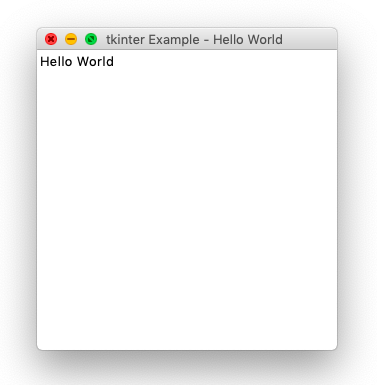
\includegraphics[width=0.8\textwidth]{images/HelloWorldGUI.png}
	\caption{Hello World Beispiel mit grafischer Benutzeroberfl�che}
	\label{ui:helloWorld:img:helloWorldGUI}
\end{figure}

Das Programm wird nun solange ausgef�hrt und bleibt in der Ereignisschleife, bis das Fenster geschlossen wird.
In dieser Schleife werden nicht nur Events wie Nutzereingaben (z.B. Mausklicks oder Tastatureingaben)
verarbeitet, sondern auch die des Fenstersystems (z.B. Redraw-Ereignisse und Fenster-Konfigurationsmeldungen) und
Ereignisse von Tkinter selbst.

\uebung
\aufgabe{UI_aufgabe01}


\section{Die Layout-Manager}
\label{ui:layoutManager:section:dieLayoutManager}

In diesem Kapitel werden die Layout- oder Gemeometrie-Manager von Tkinter behandelt.
Grunds�tzlich stehen drei verschiedene Layout-Manager zur Verf�gung:

\begin{itemize}
    \item Pack
    \item Grid
    \item Place
\end{itemize}

Layout-Manager dienen in erster Linie dazu, Widgets in einem Wurzel-Element zu regestrieren,
anzuordnen und darzustellen. Besonders die Anordnung durch Angabe von Position und Gr��e eines Widgets
wird durch die Layout-Manager stark vereinfacht.

Einem Wurzel-Element sollte immer nur ein Layout-Manager angeh�ngt werden.

\subsection{Pack}
\label{ui:layoutManager:subsection:pack}

Der Pack-Manager ist der am einfachsten zu verwendende Layout-Manager.
Hier werden Widgets in Zeilen oder Spalten (vertikal oder horizontal) 'gepackt' und durch Optionen wie
\lstinline$fill$ oder \lstinline$expand$ gesteuert.

Im Vergleich zu dem sehr �hnlichen Grid-Manager ist der Pack-Manager etwas eingeschr�nkt,
aber in einigen wenigen Situationen sinnvoller zu nutzen. Speziell wenn einfache
Widgets �bereinander oder nebeneinander angeordnet werden oder Inhalte eines Widgets das gesamte
�bergeordnete Widget ausf�llen sollen, wird der Pack-Manager bevorzugt.

Das folgende Beispiel soll die Effekte des Pack-Managers verdeutlichen:

\lstinputlisting[language=Python]{chapters/userInterface/src/GUI_PackExample.py}
\label{ui:layoutManager:lst:lstinputlisting:gui_packExample}

\begin{figure}[ht]
	\centering
	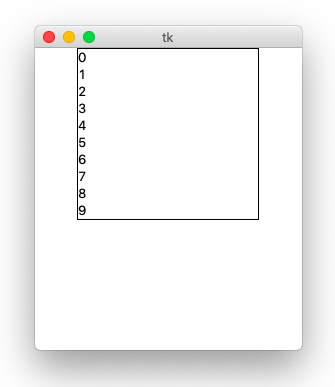
\includegraphics[width=0.5\textwidth]{images/PackManagerGUI_II.png}
	\caption{Listbox Widget mit einem Pack-Manager angeordnet}
	\label{ui:layoutManager:img:PackManagerGUI_II}
\end{figure}

Standardm��ig wird die Gr��e der Listbox so gew�hlt, dass zehn Elemente angezeigt
werden k�nnen. Im obigen Quelltext werden der Listbox allerdings doppelt so viele Elemente
�bergeben. Versucht der User nun das Wurzel-Element, sprich das Fenster, zu verg��ern,
um alle Elemente anzuzeigen, erzeugt Tkinter rund um das Listbox-Widget einen Abstand zum Fenster.
Um das Widget der gesamten zur Verf�gung stehenden Fl�che anzupassen, m�ssen die
Optionen \lstinline$fill$ und \lstinline$expand$ des Pack-Managers angesprochen werden.

\lstinputlisting[language=Python]{chapters/userInterface/src/GUI_PackExampleII.py}
\label{ui:layoutManager:lst:lstinputlisting:gui_packExampleII}

\begin{figure}[ht]
	\centering
	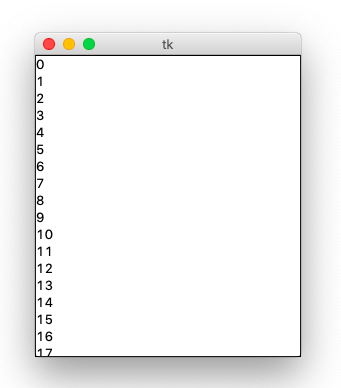
\includegraphics[width=0.5\textwidth]{images/PackManagerGUI_I.png}
	\caption{Listbox Widget mit einem Pack-Manager angeordnet unter Angabe von \lstinline$fill$ und \lstinline$expand$}
	\label{ui:layoutManager:img:PackManagerGUI_I}
\end{figure}

Die \lstinline$fill$-Option teilt dem Pack-Manager mit, dass der gesamte zur Verf�gung
stehende Raum durch das Widget ausgef�llt werden soll. Der dahinter stehende Wert
regelt, wie der Raum gef�llt wird. \lstinline$BOTH$ bedeutet, dass das Widget
sowohl horizontal als auch vertikal expandieren soll.
Alternativ kann der Raum mit der Angabe \lstinline$X$ nur horizontal und mit der Angabe
\lstinline$Y$ nur vertikal ausgef�llt werden.

Dar�ber hinaus k�nnen Widgets mithilfe der Layout-Manager angeordnet werden.
Der Pack-Manager richtet Widgets, ohne weitere Angaben von Optionen, vertikal, sprich in Spalten aus.

\lstinputlisting[language=Python]{chapters/userInterface/src/GUI_PackExampleIII.py}
\label{ui:layoutManager:lst:lstinputlisting:gui_packExampleIII}

\begin{figure}[ht]
	\centering
	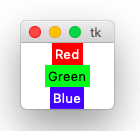
\includegraphics[width=0.3\textwidth]{images/PackManagerGUI_III.png}
	\caption{Mit Pack-Manager vertikal angeordnete Label-Widgets}
	\label{ui:layoutManager:img:PackManagerGUI_III}
\end{figure}

�ber die Option \lstinline$fill=X$ (horizontal) kann die Breite der Labels dem Eltern-Element angepasst werden.

\lstinputlisting[language=Python]{chapters/userInterface/src/GUI_PackExampleIV.py}
\label{ui:layoutManager:lst:lstinputlisting:gui_packExampleIV}

\begin{figure}[ht]
	\centering
	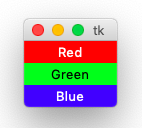
\includegraphics[width=0.3\textwidth]{images/PackManagerGUI_IV.png}
	\caption{Mit Pack-Manager vertikal angeordnete Label-Widgets unter Angabe von \lstinline$fill$}
	\label{ui:layoutManager:img:PackManagerGUI_IV}
\end{figure}

Neben der vertikalen Ausrichtung der Labels ist auch eine horizontale m�glich, dazu steht
die \lstinline$side$-Option zur Verf�gung. Mit \lstinline$side=LEFT$ werden die
Widgets von links beginnend angeordnet. Weitere Paramter sind \lstinline$side=TOP$ (default),
\lstinline$side=BOTTOM$ und \lstinline$side=RIGHT$.

\subsection{Grid}
\label{ui:layoutManager:subsection:grid}

Der Grid-Manager ist der am flexibelsten einzusetzende Layout-Manager von Tkinter.
Besonders komfortabel ist der Einsatz bei dem Gestalten von Dialogfeldern. Die Handhabung
ist denkbar einfach. Das folgende Schaubild erl�utert die Aufteilung eines Gitterrasters:

\begin{figure}[ht]
	\centering
	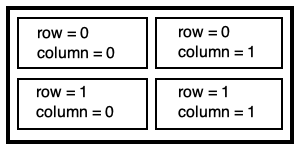
\includegraphics[width=0.4\textwidth]{images/GridManagerGUI.png}
	\caption{Gitterraster mit zwei Spalten und Reihen}
	\label{ui:layoutManager:img:GridManagerGUI}
\end{figure}

Nach dem Erzeugen eines Widget-Elements kann es �ber den Methoden-
Aufruf des Grid-Managers, unter Angabe von Zeilen und Spalten ausgerichtet
werden. Dabei muss weder H�he noch Breite der entsprechenden Zelle angegeben werden, der
Grid-Manager passt diese dem Content des Widgets an.

\lstinputlisting[language=Python]{chapters/userInterface/src/GUI_GridExampleI.py}
\label{ui:layoutManager:lst:lstinputlisting:gui_gridExampleI}

\begin{figure}[ht]
	\centering
	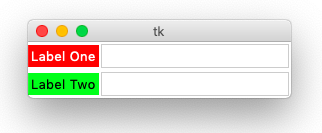
\includegraphics[width=0.5\textwidth]{images/GridManagerGUI_I.png}
	\caption{Mit Grid-Manager angeordnete Label- und Input-Widgets}
	\label{ui:layoutManager:img:GridManagerGUI_I}
\end{figure}

Leere Spalten und Zeilen werden von dem Layout-Manager ignoriert, das Ergebnis w�re
das selbe, wenn die Angabe anstelle von \lstinline$grid(row=0)$ und \lstinline$grid(row=1)$,
\lstinline$grid(row=5)$ und \lstinline$grid(row=10)$ lauten w�rde.

Der Inhalt der Zellen wird ohne weitere Angaben mittig angeordnet, was �ber die \lstinline$sticky$-Option
ge�ndert werden kann. Im Gegensatz zu der \lstinline$side$-Option des Pack-Managers,
nimmt \lstinline$sticky$ Himmelsrichtungen, also N, E, S und W als Angabe entgegen.
Mit \lstinline$Label(...).grid(row=0, sticky=W)$
beginnt der Text des Label-Widgets am linken Zellenrand (Westen). Auch Kombinationen wie beispielsweise
'unten links' (\lstinline$sticky=W+S$) sind m�glich.

\subsection{Place}
\label{ui:layoutManager:subsection:place}

Der dritte Layout-Manager von Tkinter ist der Place-Manager. Hier kann die Position und Gr��e eines
 Fensters explizit festgelegt werden, entweder absolut oder relativ zu einem anderen Fenster.
In der Regel werden Pack- oder Grid-Manager f�r die Gestaltung herk�mmlicher Dialog- und Fensteroberfl�chen
verwendet, in einigen wenigen F�llen ist jedoch der Place-Manager die bessere Wahl.
Beispielswei�e bei der Anordnung von Steuerelementen in Popup-Dialogen kommt der Place-Manager zum Einsatz.

Der Zugriff erfolgt wie bei ben vorherigen Layout-Managern �ber den Methodenaufruf unter Angabe
von X und Y - Koordinaten. Alternativ k�nnen mit der \lstinline$anchor$-Option �hnlich
der \lstinline$side$-Option des Pack-Managers, die Widgets �ber Kompass-Richtungen
ausgerichtet werden. Default ist NW (obere linke Ecke des Eltern-Elements).

\subsection{Zusammenfassung}
\label{ui:layoutManager:subsection:zusammenfassung}

Zusammenfassend kann gesagt werden:

\begin{itemize}
    \item Der Pack-Manger organisiert Widget-Elemente in Blocks. Anschlie�end werden diese im Eltern-Element platziert.
    \item Der Grid-Manger platziert Widget-Elemente in einer Tabellenartigen Struktur im Eltern-Element.
    \item Der Place-Manager platziert Widget-Elemente in spezifischer Position im Eltern-Element.
\end{itemize}

\uebung
\aufgabe{UI_aufgabe02}


\section{Widgets}
\label{ui:widgets:section:widgets}
Unter den Widgets werden in Tkinter alle grafischen Interaktionselemente wie Buttons, Labels,
Listboxes sowie Canvas etc. verstanden. Tkinter bietet hierf�r bereits vorgefertigte Klassen,
aus denen diese Widgets erzeugt werden k�nnen. Im Rahmen dieses Kapitels wird eine
Anwendung erstellt, die den Umgang mit einigen Widgets verdeutlichen soll und fortlaufend
dahingehend erweitert wird.

\subsection{Frame}
\label{ui:widgets:subsection:frame}
Frames fungieren, �hnlich wie die sogenannten \lstinline$divs$ in HTML, als Container um verschiedene
Widgets oder weitere Frames in einem bestimmten Bereich des Fensters zu gruppieren.
Dabei wird ein Rechteck erstellt und dem Eltern-Element �ber den Layout-Manager hinzugef�gt.
In folgendem Beispiel werden drei Frames erzeugt, die sich untereinander befinden und
unterschiedliche Hintergrundfarben besitzen. Um zu verdeutlichen, dass weitere Widgets
jetzt den jeweiligen Frame-Bereichen zugeordnet werden k�nnen, wird in jedem Frame ein
Label hinzugef�gt. Somit kann die Platzierung von Widgets besser kontrolliert werden.

\lstinputlisting[language=Python]{chapters/userInterface/src/GUI_FrameExample.py}
\label{ui:widgets:lst:lstinputlisting:gui_frameExample}

\begin{figure}[ht]
	\centering
	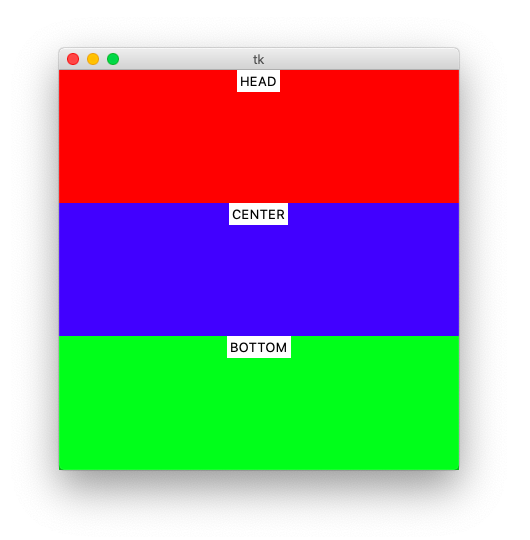
\includegraphics[width=0.5\textwidth]{images/FrameExampleGUI.png}
	\caption{Frame-Widget Beispiel}
	\label{ui:layoutManager:img:FrameExampleGUI}
\end{figure}

\subsection{Label}
\label{ui:widgets:subsection:label}
�ber Labels k�nnen im Userinterface einfache Textzeilen ausgegeben werden.
Diese lassen sich weiterhin auch dynamisch ver�ndern (z.B. bei einem Klick auf einen Button).

\subsection{Button}
\label{ui:widgets:subsection:button}
Mit dem Button hat der Nutzer die M�glichkeit, mit dem Userinterface �ber einen Maus-Klick
zu interagieren. Buttons werden aus der Klasse \lstinline$Button$ erzeugt, dem Fenster oder Frame
bekannt gemacht und mit einem Text versehen. Zus�tzlich kann dem Button �ber \lstinline$command$
noch eine Funktion zugewiesen werden, die ausgef�hrt wird, sobald der Button gedr�ckt wurde.
In folgendem Beispiel wird bei Klick auf einen Button in einem Label der Satz \lstinline$Hallo Python-World$
ausgegeben.

\lstinputlisting[language=Python]{chapters/userInterface/src/GUI_ButtonLabelExample.py}
\label{ui:widgets:lst:lstinputlisting:gui_buttonLabelExample}

\begin{figure}[ht]
	\centering
	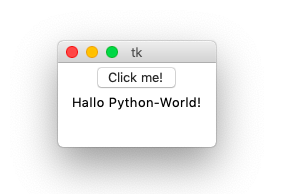
\includegraphics[width=0.5\textwidth]{images/ButtonLabelGUI.png}
	\caption{Button- und Label-Widget Beispiel}
	\label{ui:layoutManager:img:ButtonLabelGUI}
\end{figure}

\subsection{Entry}
\label{ui:widgets:subsection:entry}
�ber die sogenannten Entries lassen sich Eingaben vom Nutzer erfassen. Diese k�nnen dann im
Python-Skript weiterverarbeitet werden. Das vorherige Beispiel wird nun dementsprechend
erweitert, dass der Text, der bei Klick auf den Button ausgegeben wird, �ber \lstinline$get()$
vom Entry entgegen genommen wird.

\lstinputlisting[language=Python]{chapters/userInterface/src/GUI_EntryExample.py}
\label{ui:widgets:lst:lstinputlisting:gui_buttonLabelExample}

\begin{figure}[ht]
	\centering
	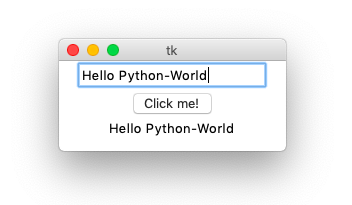
\includegraphics[width=0.5\textwidth]{images/EntryExampleGUI.png}
	\caption{Entry-Widget Beispiel}
	\label{ui:layoutManager:img:EntryExampleGUI}
\end{figure}

\subsection{Listbox}
\label{ui:widgets:subsection:listbox}
Um verschiedene Elemente in einer Liste anzeigen zu k�nnen, bietet sich die Listbox an.
Der Text, der vom Entry entgegengenommen wird, soll nun einer solchen Listbox hinzugef�gt werden.
Dazu dient die Funktion \lstinline$insert()$. Der erste Parameter, der �bergeben wird, bestimmt
die Position in der Liste und der zweite das eigentliche Element.
Zus�tzlich wird der Anwendung ein zweiter Button hinzugef�gt um das jeweilig angew�hlte Element
der Listbox zu entfernen. Die Funktion \lstinline$curselection()$ gibt eine Liste der angew�hlten
Elemente zur�ck. Mithilfe von \lstinline$delete()$ wird dann das erste Element der zur�ckgegebenen Liste
aus der Listbox entfernt.

\lstinputlisting[language=Python]{chapters/userInterface/src/GUI_ListboxExample.py}
\label{ui:widgets:lst:lstinputlisting:gui_listboxwExample}

\begin{figure}[ht]
	\centering
	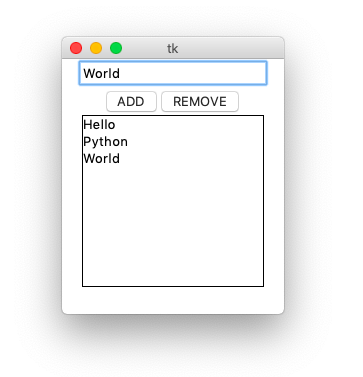
\includegraphics[width=0.5\textwidth]{images/ListboxExampleGUI.png}
	\caption{Listbox-Widget Beispiel}
	\label{ui:layoutManager:img:ListboxExampleGUI}
\end{figure}

\subsection{Colorchooser}
\label{ui:widgets:subsection:colorchooser}
Das Colorpicker oder Colorchooser-Modul bietet die M�glichkeit Farben auszuw�hlen.
Diese kann anschlie�end �ber die Methode \lstinline$askcolor()$
ausgelesen und Beispielsweise einem weiteren Widget �bergeben werden. Es handelt
sich um ein Tupel der Form \lstinline$((99, 222, 170), �#63deaa�)$, wobei der erste
Teil die RGB-Werte und der zweite Teil den hexadezimal Farbcode verk�rpert.
Das Colorchooser-Modul von Tkinter bietet eine Schnittstelle zum nativen Farbauswahl-Widget
des zugrundeliegenden Systems, weshalb sich das Widget in Optik und Funktion je nach Betriebssystem
unterscheiden kann. Der Colorchooser wird �ber \lstinline$tkinter.colorchooser$ importiert.

\begin{figure}[ht]
	\centering
	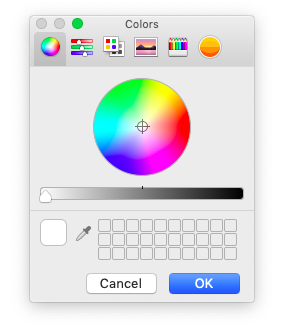
\includegraphics[width=0.5\textwidth]{images/ColorchooserGUI.png}
	\caption{Colorchooser-Widget unter macOS}
	\label{ui:layoutManager:img:ColorchooserGUI}
\end{figure}

\subsection{Canvas}
\label{ui:widgets:subsection:canvas}
Analog zu dem in HTML 5 eingef�hrten Canvas-Widget oder Canvas-Element bietet auch
Tkinter ein Element zur Darstellung verschiedener grafischer Objekte.
Mithilfe von Canvas k�nnen Linien, Kreise oder aufwendige Formen in einem daf�r
vorgesehenen Rahmen angezeigt werden. Dabei stehen mehrere Methoden zum gestalten
grafischer Objekte zur Verf�gung. Mit \lstinline$create_line()$ k�nnen Linien,
mit \lstinline$create_oval()$ oder \lstinline$create_rectangle()$ fertige geometrische
Formen erstellt und anschlie�end dem Canvas zum Zeichnen �bergeben werden.
\lstinline$Create_polygon()$ bietet sogar die M�glichkeit ganze Polygonz�ge und
somit uneingeschr�nkte, zweidimensionale Figuren zu erstellen. Dabei muss als erstes
Argumt eine Reihe von kartesischen Koordinaten �bergeben werden. Im folgenden Beispiel
wird ein blaues Dreieck erstellt und anschlie�end gezeichnet:

\lstinline$canvas.create_polygon([120, 120, 220, 220, 220, 120], blue)$

\begin{figure}[ht]
	\centering
	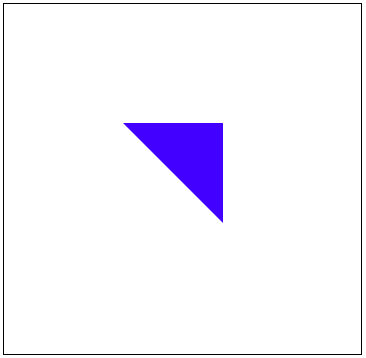
\includegraphics[width=0.5\textwidth]{images/CanvasGUI.png}
	\caption{Ein Mithilfe der Create Polygon Canvas-Methode erstelltes Dreieck}
	\label{ui:layoutManager:img:CanvasGUI}
\end{figure}

Um ein gezeichnetes Objekt zu l�schen bzw. die Zeichenfl�che zu reinigen steht
die Methode \lstinline$canvas.delete(ALL)$ zur Verf�gung. Der �bergabe Parameter
besagt dabei, alle Objekte die dem Widget �bergeben wurden sollen gel�scht werden.

\uebung
\aufgabe{UI_aufgabe03}
\aufgabe{UI_aufgabe04}
\aufgabe{UI_aufgabe05}
\aufgabe{UI_aufgabe06}
\aufgabe{UI_aufgabe07}
\aufgabe{UI_aufgabe08}
\aufgabe{UI_aufgabe09}


% !TeX root = ../pythonTutorial.tex
\chapter{Python Bibliotheken}

\label{bibliotheken:numpy}
\section{NumPy}
\label{numpy}
NumPy ist eine Python-Bibliothek f�r wissenschaftliches Rechnen.
Sie beinhaltet laut der Dokumentation unter anderem Folgendes \cite{numpy}:

\begin{itemize}
  \item m�chtige $n$-dimensionale Array-Objekte
  \item Werkzeuge zur Integration von C und Fortran
  \item Funktionen zur linearen Algebra, Fouriertransformation, Erzeugung von
        Zufallszahlen
\end{itemize}

% Zitat: http://www.numpy.org

Um NumPy zu installieren, kann der Befehl \lstinline!pip install numpy!
verwendet werden.

\subsection{Arrays}
\label{numpy:subsection:arrays}

Der Array-Datentyp von NumPy hei�t \lstinline!numpy.ndarray!.
Anders als der Standarddatentyp f�r Listen (\lstinline!list!) unterst�tzt der
Datentyp \lstinline!numpy.ndarray! numerische Operatoren.
Der NumPy-eigene Datentyp erm�glicht es, Arrays direkt �ber den
\lstinline!+!-Operator elementweise zu addieren. Eine Addition mit einer
einzelnen Zahl vom Typ \lstinline!int! oder \lstinline!float! betrifft alle
Elemente im Array.

So kann etwa jeder Wert in einem Array mit den folgenden Anweisungen um drei
erh�ht werden:
\begin{lstlisting}
import numpy as np
a = np.array([1,2,3])
a + 3 # [4 5 6]
\end{lstlisting}
NumPy wird hierbei mit dem Namen \lstinline!np! importiert. Damit folgt dieses
Tutorial der Konvention aus der Dokumentation von NumPy.

Subtraktion, Multiplikation, Division, Ganzzahldivision und Potenzieren
funktionieren analog:\footnote{Der Import von \lstinline!numpy! wird der
�bersichtlichkeit halber nachfolgend ausgelassen.}
\begin{lstlisting}
a = np.array([1,2,3])
a - 3  # [-2 -1  0]
a * 3  # [3 6 9]
a / 3  # [0.33333333 0.66666667 1.        ]
a // 3 # [0 0 1]
a ** 3 # [ 1  8 27]
\end{lstlisting}

Zwei Arrays gleicher L�nge k�nnen elementweise miteinander verrechnet werden:
\begin{lstlisting}
a = np.array([1,2,3])
b = np.array([4,5,6])
a + b  # [5 7 9]
a - b  # [-3 -3 -3]
a * b  # [ 4 10 18]
a / b  # [0.25 0.4  0.5 ]
a ** b # [  1  32 729]
a // b # [0 0 0]
\end{lstlisting}

Um ein NumPy-Array zu erzeugen, wird ein \lstinline!list!-Objekt an die Funktion
\lstinline!np.array()! �bergeben. Dabei werden alle Elemente im
\lstinline!list!-Objekt in einem Datentyp von NumPy konvertiert. Um den Datentyp
eines Arrays herauszufinden, wird \lstinline!.dtype.name! genutzt. Anders
als bei \lstinline!list! m�ssen s�mtliche Elemente eines Arrays den gleichen
Typ haben.
\begin{lstlisting}
a = np.array([1,2,3])
a.dtype.name # 'int64'
b = np.array([1.4,2.5,3.6])
a.dtype.name # 'float64'
\end{lstlisting}

Wenn die �bergebene \lstinline!list! Elemente vom Typ \lstinline!int! und von
Typ \lstinline!float! gemischt enth�lt,
konvertiert NumPy in einen Flie�kommatyp. Wie viele Bit f�r einen Integer
beziehungsweise ein Float zur Verf�gung stehen, ist von der Prozessorarchitektur
abh�ngig. Diese betr�gt aber bei aktuellen Architekturen in der Regel 64 Bit.

\subsection{Konstanten und Funktionen}
\label{numpy:subsection:constantsAndFunctions}
Es stehen f�r die mathematische Anwendungen auch Konstanten zur Verf�gung,
darunter die Folgenden mit den entsprechenden Werten und Pr�zisionen mit
\lstinline!float64!:
\begin{lstlisting}
>>> np.pi
3.141592653589793
>>> np.e
2.718281828459045
>>> np.euler_gamma
0.5772156649015329
>>> np.PINF
inf
>>> np.NINF
-inf
>>> np.NAN
nan
>>> np.PZERO
0.0
>>> np.NZERO
-0.0
>>> np.NAN
nan
\end{lstlisting}
\lstinline!np.NZERO! steht f�r die negative Darstellung der Null bei
Flie�kommazahlen, \lstinline!np.PZERO! f�r die positive Darstellung.

NumPy unterst�tzt eine Vielzahl an mathematischen Funktionen, darunter unter
anderem Folgende:

\begin{itemize}
  \item trigonometrische Funktionen
  \item Rundungsfunktionen
  \item Summationsfunktionen
  \item Multiplikationsfunktionen
  \item Funktionen zur Behandlung komplexer Zahlen
\end{itemize}

Die grundlegenden trigonometrischen Funktionen werden elementweise auf das Array
angewendet:
\begin{lstlisting}
>>> a = np.array([0, np.pi/6, np.pi/4, np.pi/3, np.pi/2])
>>> np.sin(a)
[0.         0.5        0.70710678 0.8660254  1.        ]
>>> np.cos(a)
[1.00000000e+00 8.66025404e-01 7.07106781e-01 5.00000000e-01
6.12323400e-17]
>> np.tan(a)
[0.00000000e+00, 5.77350269e-01, 1.00000000e+00,
1.73205081e+00, 1.63312394e+16]
\end{lstlisting}

Umrechung von Radians in Grad:
\begin{lstlisting}
>>> a = np.array([0, np.pi/6, np.pi/4, np.pi/3, np.pi/2])
>>> np.degrees(a)
[ 0., 30., 45., 60., 90.]
\end{lstlisting}
Umrechung von Grad in Radians:
\begin{lstlisting}
>>> a = np.array([ 0, 30, 45, 60, 90])
>>> np.radians(a)
[0.         0.52359878 0.78539816 1.04719755 1.57079633]
\end{lstlisting}

Mit der Funktion \lstinline!np.around()! k�nnen s�mtliche Werte im Array auf
eine bestimmte Anzahl von Stellen gerundet werden. Ohne Angabe eines zweiten
Arguments wird kaufm�nnisch auf die n�chste Ganzzahl gerundet.
\begin{lstlisting}
>>> a = np.array([1.49, 1.5, 1.51])
>>> np.around(a)
[1. 2. 2.]
\end{lstlisting}
Mit dem optionalen zweiten Argument wird die Anzahl an Nachkommastellen, auf die
gerundet werden soll, angegeben:
\begin{lstlisting}
>>> a = np.array([1.25, 1.53, 1.99])
>>> np.around(a, 1)
[1.2, 1.5, 2. ]
\end{lstlisting}

Um alle Elemente eines Arrays aufzusummieren, wird die Funktion \\
\lstinline!np.sum()! verwendet.
\begin{lstlisting}
>>> a = np.array([1, 2, 3])
>>> np.sum(a)
6
\end{lstlisting}
Mit der Funktion \lstinline!np.prod()! k�nnen die Elemente der Liste miteinander
multipliziert werden.
\begin{lstlisting}
>>> a = np.array([2, 3, 4])
>>> np.prod(a)
24
\end{lstlisting}


Sollten \lstinline!nan! (not a number) im Array vorkommen k�nnen, so kann
die Funktion \lstinline!np.nansum()! beziehungsweise \lstinline!np.nanprod()!
verwendet werden. Bei der Funktion \lstinline!np.nansum()! werden
\lstinline!nan! als \lstinline!0! interpretiert.
\begin{lstlisting}
>>> a = np.array([np.NAN, 1, 2, 3])
>>> np.sum(a)
nan
>>> np.nansum(a)
6.0
\end{lstlisting}
Durch die Funktion \lstinline!np.nanprod()! werden \lstinline!nan! als
\lstinline!1! interpretiert:
\begin{lstlisting}
>>> a = np.array([np.NAN, 2, 3, 4])
>>> np.prod(a)
nan
>>> np.nanprod(a)
24.0
\end{lstlisting}
Addition und Multiplikation geben eine Zahl vom Typ \lstinline!float64! als
Ergebnis zur�ck. \lstinline!nan! ist ein valider Flie�zahlwert, daher werden
die restlichen Werte ebenfalls nach \lstinline!float64! konvertiert.

\subsection{Erzeugen und Manipulieren von Arrays}
\label{numpy:subsection:createAndManipulateArrays}

Bislang haben die Beispiele in diesem Kapitel Arrays immer auf die folgende
Weise erzeugt:
\begin{lstlisting}
>>> a = np.array([1,2,3])
>>> a
[1 2 3]
\end{lstlisting}
Hierbei wird zuerst eine \lstinline!list! mit konkreten Werten erzeugt und dann
mittels \lstinline!np.array! in ein NumPy-Array konvertiert.

Neben Listen kann \lstinline!np.array! auch s�mtliche anderen Sequences in
Arrays umwandeln, zum Beispiel Tupel und Ranges:
\begin{lstlisting}
>>> t = (1, 2, 3)
>>> np.array(t)
[1, 2, 3]
>>> r = range(1,6)
>>> np.array(r)
[1, 2, 3, 4, 5]
\end{lstlisting}

Numpy kann auch direkt ein Numpy-Array mit den gleichen Paramtern wie von
\lstinline!range! erzeugen. Die Funktion hierzu hei�t \lstinline!np.arange()!:
\begin{lstlisting}
>>> np.arange(1,6)
[1, 2, 3, 4, 5]
\end{lstlisting}

Ebenso k�nnen mehrdimensionale Arrays erzeugt werden:
\begin{lstlisting}
>>> a = [[1, 2], [3, 4]]
>>> np.array(a)
[[1 2]
 [3 4]]
\end{lstlisting}

�ber das Attribut \lstinline!.shape! kann jederzeit die Form eines Arrays
abgefragt werden.
\begin{lstlisting}
>>> a = [[1, 2], [3, 4]]
>>> b = np.array(a)
>>> b.shape
(2, 2)
\end{lstlisting}

\subsubsection{Leere Arrays}

Wenn die Werte des Arrays zum Zeitpunkt seiner Erzeugung noch nicht bekannt
sind, kann mit der Funktion \lstinline!np.empty()! ein leeres Array erzugt
werden. Welche Werte dabei initial im Array stehen, ist nicht definiert, da
\lstinline!np.empty()! lediglich das Array erzeugt, nicht aber dessen Werte
initialisiert. Die Werte eines so erzeugten Arrays sind zuf�llig.
\begin{lstlisting}
>>> np.empty(2)
[1.13224202e+277, 2.00000008e+000]
\end{lstlisting}

Bei den Funktionen in diesem Abschnitt kann statt einer Zahl als L�nge auch eine
Sequence mit den L�ngen der Dimensionen �bergeben werden:
\begin{lstlisting}
>>> np.empty([2,3])
[[ 1.,  4.,  9.]
 [16., 25., 36.]]
\end{lstlisting}

Der Paramter bestimmt die L�nge des Arrays, der Datentyp ist standardm��ig
\lstinline!float64!. Um ein \lstinline!int64!-Array zu erzeugen, wird das
optionale Argument \lstinline!dtype=int! mit �bergeben:
\begin{lstlisting}
>>> np.empty(2, dtype=int)
[8751743591039004782, 4611686018597859880]
\end{lstlisting}

\warning{Diese Funktion sollte mit Vorsicht genutzt werden, da die Werte manuell
gesetzt werden m�ssen!}

Analog zu \lstinline!np.empty()! kann bei den allen Funktionen zur Erzeugung
von Arrays der Datentyp explizit angegeben werden:
\begin{lstlisting}
>>> np.array([1, 2], dtype=float)
array([1., 2.])
\end{lstlisting}
Neben \lstinline!int! und \lstinline!float! kann bei Bedarf mit
\lstinline!np.int8!, \lstinline!np.int16!, \lstinline!np.int32!,
\lstinline!np.int64!, \lstinline!np.float16!, \lstinline!np.float32!,
\lstinline!np.float64! und \lstinline!np.float128! explizit die Gr��e des
Integer beziehungsweise Float-Wertes im Speicher bestimmt werden.

Besonders interessant ist hierbei \lstinline!np.float128!, ein Float mit
Quadruple Precision und 128 Bit L�nge. Damit k�nnen mindestens 34 Stellen
Pr�zision gepeichert werden.\footnote{F�r die Mantisse stehen beim
\texttt{np.float64} nach IEEE 754 113 Bit zur Verf�gung. Das ergibt aufgrund
von $\log_{10}(2^{113})\approx34.016$ 34 Stellen.}

\subsubsection{Arrays mit Standardwerten}

Die Funktion \lstinline!np.ones()! erzeugt Arrays, die mit Einsen initialisiert
sind:
\begin{lstlisting}
>>> np.ones(7)
[1., 1., 1., 1., 1., 1., 1.]
\end{lstlisting}

Mit \lstinline!np.zeros()! werden Arrays mit Nullen gef�llt:
\begin{lstlisting}
>>> np.zeros(7)
[0., 0., 0., 0., 0., 0., 0.]
\end{lstlisting}

Die Funktion \lstinline!np.full()! f�llt ein Array mit dem angegebenen Wert:

\begin{lstlisting}
>>> np.full(3, np.pi)
[3.14159265, 3.14159265, 3.14159265]
\end{lstlisting}

\subsubsection{Arrays kopieren}

Um ein vorhandenes Array zu kopieren, wird die \lstinline!.copy()!-Methode
verwendet.
\begin{lstlisting}
>>> a = np.array([1,2,3])
>>> b = a
>>> c = a.copy()
>>> print(a, b, c)
[1 2 3] [1 2 3] [1 2 3]
>>> a += 3
>>> print(a, b, c)
[4 5 6] [4 5 6] [1 2 3]
\end{lstlisting}
Mit dem Zuweisungsoperator wird lediglich eine Referenz auf das Array erzeugt,
die Methode \lstinline!.copy()! erzeugt eine Objektkopie.

\subsubsection{Arrays persistieren}

Um Arrays zu persistieren, k�nnen die Funktionen \lstinline!np.save()! zum
Speichern und \lstinline!np.load()! zum Auslesen verwendet werden. Das
nachfolgende Beispiel simuliert dieses Verhalten mit der Klasse
\lstinline!TemporaryFile! aus dem \lstinline!tmpfile!-Paket.
\lstinline!TemporaryFile! verh�hlt sich wie eine normale Datei, mit dem
Unterschied, dass der Dateiinhalt im Arbeitsspeicher vorgehalten wird. Mit der
Methode \lstinline!.seek(0)! auf ein \lstinline!TemporaryFile!-Objekt wird das
Schlie�en und erneute �ffnen der Datei
simuliert.
\begin{lstlisting}
>>> from tempfile import TemporaryFile
>>> outfile = TemporaryFile()
>>> a = np.array([1,2,3,4])
>>> np.save(outfile, a)
>>> outfile.seek(0)
>>> np.load(outfile)
[1, 2, 3, 4]
\end{lstlisting}
Per Konvention lautet die Dateiendung so gespeichter Arrays \lstinline!.npy!.

\subsubsection{Arrays mittels Funktionen berechnen}

Mit der Funktion \lstinline!np.fromfunction()! k�nnen die Werte mittels einer
gebenen Funktion berechnet werden. Dabei sind die Parameter der Funktion die
Indizes der Position im Array. Die Dimensionen des Arrays \emph{m�ssen} bei
\lstinline!np.fromfunction()! als Sequence �bergeben werden. Wenn kein Datentyp
angegen wird, wird \lstinline!np.float64! angenommen.
\begin{lstlisting}
>>> f = lambda i: i ** 2
>>> np.fromfunction(f, [7], dtype=int)
array([ 0,  1,  4,  9, 16, 25, 36])
\end{lstlisting}

Die Form des Arrays ist bei \lstinline!np.fromfunction()! abh�ngig von der
verwendeten Funktion. Wenn diese skalare Werte zur�ckgibt, entspricht die Form
den in den Paramtern angegebenen Dimensionen.
\begin{lstlisting}
>>> f = lambda i, j: i + j
>>> a = np.fromfunction(f, [3, 2], dtype=int)
[[0 1]
 [1 2]
 [2 3]]
>>> a.shape
(3, 2)
\end{lstlisting}

Untenstehendes Beispiel zeigt, wie sich die Form des Arrays durch die
R�ckgabewerte der Funktion ver�ndern kann.
\begin{lstlisting}
>>> f = lambda i, j: np.array([i, j])
>>> a = np.fromfunction(f, [3, 2], dtype=int)
>>> a
[[[0 0]
  [1 1]
  [2 2]]

 [[0 1]
  [0 1]
  [0 1]]]
>>> a.shape
(2, 3, 2)
\end{lstlisting}

\subsubsection{Arrays aus iterierbaren Objekten erzeugen}

Um ein beliebiges iterierbares Objekt in ein eindimensionales Array zu
konvertieren, bietet NumPy die Funktion \lstinline!np.fromiter()! an. Der zweite
Parameter gibt den Datentyp des Arrays an. Mit dem
optionalen Parameter \lstinline!count! wird angegeben, wie viele Elemente aus
dem Objekt �bernommen werden sollen. Wird \lstinline!count! weggelassen, so
werden alle Werte �bernommen.
\warning{Falls das iterierbare Objekt unendlich viele Werte erzeugen kann, muss
\lstinline!count! angegeben werden, da \lstinline!np.fromiter()! sonst niemals
abbricht!}

\begin{lstlisting}
>>> def even_numbers():
...     i = 0
...     while True:
...         yield i
...         i += 2
...
>>> np.fromiter(even_numbers(), int, count=10)
[ 0,  2,  4,  6,  8, 10, 12, 14, 16, 18]
\end{lstlisting}

\uebung
\aufgabe{numpy_01}
\aufgabe{numpy_02}



% !TeX root = ../../pythonTutorial.tex

\chapter{Dokumentation}
\label{documentation:sec:Dokumentation}

Wie in allen Programmiersprachen ist vor allem bei gro�en Programmen eine gute Dokumentation wichtig.
Viele Funktionen sind ohne ausreichende Beschreibungen nicht gut nachvollziehbar und man kann oft nur erahnen, was ein bestimmter Programmteil letztendlich bewirkt.
Da von vielen Programmierern aus Bequemlichkeit und Schreibfaulheit auf eine umfassende Dokumentation verzichtet wird, sind viele Programme kaum bis �berhaupt nicht wartbar oder ver�nderbar.

In Python gibt es f�r genau dieses Problem Tools, mit dessen Hilfe die Dokumentation von Programmen auf ein angenehmes Ma� reduziert wird.
Eines dieser plattformunabh�ngigen Werkzeuge mit dem Namen \textit{epydoc} wird im Folgenden genauer betrachtet.
\randnotiz{epydoc} epydoc analysiert Python-Programme anhand des Quellcodes, verwertet diesen und gibt anschlie�end eine Dokumentation als PDF- oder HTML-Datei aus.
Bei dieser Analyse werden Doc- strings ben�tigt, deren Benutzung und Einbindung noch genauer betrachtet wird.

Unter \url{http://epydoc.sourceforge.net} k�nnen Sie sich die aktuelle epydoc-Version herunterladen und anschlie�end installieren.


\section{Epydoc}
\label{documentation:sec:epydoc}

Nach der erfolgreichen Installation kann epydoc �ber die Konsole aufgerufen werden.
Dazu wird der Befehl \textit{epydoc.py} benutzt. (in Linux ohne .py)
Eine Dokumentation zu einer bestimmten Python-Datei ist dann m�glich, wenn epydoc an der selben Stelle im Dateipfad ausgef�hrt wird.

Um das Format zwischen PDF und HTML zu wechseln, wird der Befehl \textit{--pdf} beziehungsweise \textit{--html} verwendet.
Auch den Speicherort der Dokumentation kann frei variiert werden.
Dazu wird der Befehl \textit{--output} vor den gew�nschten Verzeichnisort geschrieben.

Ein Beispiel f�r eine korrekte Dokumentationserstellung durch epydoc sieht wie folgt aus:
\begin{lstlisting}[label=documentation:lst:epydocbsp]
$ epydoc.py --html --output eigenes_verzeichnis testprogramm
\end{lstlisting}
Dadurch wird die Dokumentation zum Modul \textit{testprogramm} als HTML-Datei im Verzeichnis \textit{gewuenschtesverzeichnis} gespeichert.


\section{Docstrings}
\label{documentation:sec:docstrings}

Python bietet uns durch drei einfache oder doppelte Anf�hrungszeichen die M�glichkeit, sogenannte Blockkommentare �ber mehrere Zeilen zu verfassen.
Der darin eingefasste Text wird als Documentation String, kurz \textit{Docstring} bezeichnet.

\begin{lstlisting}[label=documentation:lst:docstringbsp]
"""
Dieser Text ist ein Docstring.
Er wird von epydoc als solcher erkannt,
analysiert und interpretiert.
"""
\end{lstlisting}

Docstrings sollten zur Beschreibung aller Programmierteile benutzt werden, vor allem Funktionen und Klassen sollten durchgehend kommentiert werden.

\begin{lstlisting}[label=documentation:lst:docstringbsp2]
class myclass(object):
   """Docstring zur Klasse myclass
   Beschreibung, wozu die Klasse dient.
   """

def myfunction():
   """Docstring zur Funktion myfunction
   Beschreibung, was die Funktion macht.
   """
\end{lstlisting}

Innerhalb des Programms kann man durch einen Befehl einen beliebigen Docstring aufrufen.
Dazu dient das Attribut \_doc\_, das zu jeder Instanz automatisch erstellt wird.

\begin{lstlisting}[label=documentation:lst:docstringausgeben]
>>> print myclass.__doc__
Docstring zur Klasse myclass
   Beschreibung, wozu die Klasse dient.
\end{lstlisting}


Python hat intern jedoch keine M�glichkeit, um f�r Variablen Docstrings zu nutzen.
Diese M�glichkeit wird durch epydoc erm�glicht.
Folgt in der folgenden Zeile nach einer Variablenzuweisung ein Blockkommentar, wird dieser automatisch als Docstring zur Variablen interpretiert.
Eine weitere M�glichkeit ist es, den Docstring vor die Wertezuweisung der Variablen zu definieren.
In diesem Fall wird auf die dreifachen Anf�hrungszeichen verzichtet und je Zeile eine Raute mit Doppelpunkt \#: vorangestellt.

\begin{lstlisting}[label=documentation:lst:docstringepydoc]
a = 42
""" Die Variable a ist 42
"""

#: Die Variable b
#: ist 24
b = 24
\end{lstlisting}


\section{Epytext}
\label{documentation:sec:Epytext}
Um sicherzustellen, dass epydoc die Docstrings richtig interpretiert, wurde die Beschreibungssprache Epytext eingef�hrt.
Darin sind Regeln f�r die Formatierung und die Umsetzung mit Docstrings festgehalten, um eine einheitliche Benutzung zu gew�hrleisten.
Im Folgenden werden einige der Regeln und M�glichkeiten betrachtet.

Zum einen ist in Epytext, genau wie in Python die korrekte Einr�ckung von entscheidender Wichtigkeit.

\begin{lstlisting}[label=documentation:lst:einrueckung]
def myfunction():
   """
   Wichtig ist die richtige Einr�ckung
   """
\end{lstlisting}

Auch Listen sind innerhalb von Docstrings m�glich.
Diese k�nnen als einfache Auflistung oder  Nummerierung benutzt werden.
\begin{lstlisting}[label=documentation:lst:liste]
"""
Auflistung:
- Eier
- Milch
- Mehl

Nummerierung:
1. Aufstehen
2. Z�hne putzen
3. Duschen
"""
\end{lstlisting}

Weitere Formatierungsm�glichkeiten werden kurz in folgendem Beispiel gezeigt.
Der Aufbau ist dabei stets in der Form eines Gro�buchstabens mit dem zu formatierenden Strings in geschweiften Klammern \textit{x{*}}.

\begin{lstlisting}[label=documentation:lst:liste]
"""
I{Dieser String ist kursiv}
F{Dieser String ist fett}
M{Dies ist ein mathematischer Ausdruck}
U{String ist eine URL und wird als Hyperlink interpretiert}
E{Verhindert die Interpretation}
"""
\end{lstlisting}

\section{Zusammenfassung}
\label{documentation:sec:zusammenfassung}
Vielen Programmierern ist die st�ndige Dokumentation seit jeher ein Dorn im Auge.
Mit epydoc ist in der Python-Programmierung jedoch ein Tool vorhanden, welche einem die Arbeit zu einem gewissen Teil abnimmt.
Deshalb sollte dieses oder ein �hnliches Programm verwendet werden, um sicherzustellen, dass auch nach der Fertigstellung des Programms nachvollziehbar wird, was der eigentliche Sinn und Zweck hinter den einzelnen Programmteilen ist.
Falls Sie sich nach diesem Grund�berblick noch weiter �ber epydoc und Epytext informieren m�chten, k�nnen Sie sich die Dokumentation auf der offiziellen Homepage von epydoc anschauen.

Diese finden Sie unter \url{http//epydoc.sourceforge.net}. 

% !TeX root = ../pythonTutorial.tex
\chapter{Weiterf�hrende Themen}

% !TeX root = ../../pythonTutorial.tex
\label{machineLeaerning}

\section{Maschinelles Lernen in Python}\label{maschinelleslernen:einleitung}
Das Themengebiet des maschinellen Lernens kann verschiedene Komplexit�tslevel erreichen. Grundlegend ist das mathematische Verst�ndnis �ber die verschiedenen im maschinellen lernen eingesetzten Algorithmen. Diese werden in diesem Tutorial nicht beschrieben. \\
Sind die Algorithmen bekannt und sollen nun mittels Python angewendet werden, sollte zu Beginn mit einem kleinen Projekt gestartet werden. Hierbei ist es sinnvoll sich bereits am Anfang eine Vorgehensweise zu �berlegen, wie auch bei allen anderen Projekten. Python bietet im Bereich des maschinellen Lernens viele unterschiedliche M�glichkeiten an, sodass bereits fr�hzeitig der Aufbau des Projekts entschieden werden sollte. Grob kann ein Projekt in f�nf Schritte aufgeteilt werden, anhand derer sp�ter das Ergebnis verifiziert werden kann. \\

\begin{enumerate}
\item zu l�sendes Problem definieren
\item Daten verstehen und vorbereiten
\item m�gliche Algorithmen evaluieren
\item Ergebnisse verbessern
\item Ergebnisse darstellen
\end{enumerate}


Eine weit verbreitete M�glichkeit ist das Einbinden von bereits existierenden Bibliotheken, die viele Funktionalit�ten von Haus aus anbieten. Eine eigene Nachbildung von verbreiteten Algorithmen aus dem Bereich Maschinelles Lernen ist daher meist nicht n�tig.\\
Eine zweite M�glichkeit ist die Integration von R. Bei R handelt es sich um eine eigene Programmiersprache, welche den Schwerpunkt in mathematischen Probleml�sungen hat. Python und R lassen sich beide sowohl eigenst�ndig, also auch in Verbindung miteinander einsetzen.

Im Folgenden Abschnitt gibt es eine �bersicht, �ber wichtige und bekannte Bibliotheken aus dem Bereich maschinelles Lernen. Die Anzahl der Bibliotheken macht den Einstieg nicht ganz leicht. Die St�rken und Schw�chen der einzelnen Bibliotheken sollten betrachtet werden.

\subsection{Bibliotheken}\label{maschinelleslernen:bibliotheken}
Im Bereich maschinelles Lernen sind schon viele Bibliotheken vorhanden, die unterschiedliche Schwerpunkte in dem Bereich bedienen. Aus diesem Grund erfolgt zuerst eine �bersicht �ber verbreitete Bibliotheken.

Alle Bibliotheken\randnotiz{Download und Installation} die genutzt werden sollen m�ssen zuerst installiert werden. Hierf�r gibt es je nach Bibliothek und teilweise je nach Betriebssystem mehrere Wege. Es wird empfohlen hier aus der jeweiligen Webseite die geeignetsten Variante zu w�hlen und auszuf�hren.

Nach der Installation\randnotiz{Versionen und Kompatibilit�t} sollten alle Versionen ausgelesen und abgeglichen werden. Die Kompatibilit�t ist nicht durchgehend gew�hrleistet, das betrifft vor allem die unterschiedlichen Python-Versionen.

Der folgende Codeausschnitt zeigt ein Beispiel. Dieser kann entweder direkt in der Eingabeaufforderung bzw. Konsole nach Start von Python ausgef�hrt werden oder innerhalb einer geeigneten Entwicklungsumgebung.

\begin{lstlisting}
# Python version
import sys
print("Pyton: {}".format(sys.version))

# numpy version
import numpy
print("numpy: {}".format(numpy.__version__))

# pandas version
import pandas
print("pandas: {}".format(pandas.__version__))

# rpy2 version
import rpy2
print("rpy2: {}".format(rpy2.__version__))
\end{lstlisting}\label{maschinelleslernen:lst:printversions}

Die Ausgabe ist beispielsweise die Folgende:
\begin{lstlisting}
Pyton: 3.6.1 (v3.6.1:69c0db5, Mar 21 2017, 17:54:52) 
	[MSC v.1900 32 bit (Intel)]

numpy: 1.13.3 
pandas: 0.21.0
rpy2: 2.8.6
\end{lstlisting}\label{maschinelleslernen:lst:versions}

Auf diese Art und Weise sollten alle Bibliotheken gepr�ft werden, da so eventuelle Kompatibilit�tsprobleme oder fehlerhafte Installation fr�hzeitig erkannt werden k�nnen.

\subsubsection{Bekannte Bibliotheken}\label{maschinelleslernen:bekanntebibliotheken}
Grob kann man zwischen Datenanalyse und Visualisierung unterscheiden. Zwei bekannte Bibliotheken aus dem Bereich Datenanalyse sind \lstinline$numpy$ und \lstinline$pandas$, mit denen beispielsweise Gleichungen und Optimierungsprobleme gel�st werden k�nnen. Ergebnisse solcher Berechnungen k�nnen beispielsweise mithilfe des Moduls \lstinline$matplotlib$ visualisiert werden.~\cite{Python3}



In der Bibliothek \lstinline$numpy$~\cite{numpyreference} \randnotiz{Bibliothek numpy} wird ein flexibler Datentyp f�r mehrdimensionale Arrays zur Verf�gung gestellt. Dies erm�glicht eine effiziente Durchf�hrung von komplexen Rechnungen.

Au�erdem lassen sich Integrale berechnen, statistische Berechnungen durchf�hren und auch simulieren. All das wird f�r maschinelles Lernen ben�tigt. Da die Berechnungen mit Routinen nah an der Hardware durchgef�hrt werden, lassen sich bei entsprechender Programmierung effiziente Programme schreiben.

Die Arrays in \lstinline$numpy$ sind dreidimensional und k�nnen so eine Vielzahl von Anwendungsf�llen abbilden. Der Fokus von \lstinline$numpy$ liegt in der Datenhaltung und Manipulation von Daten. Hier speziell die numerische Manipulation aus dem Bereich der linearen Algebra. Mit den Matrizen k�nnen beispielsweise Multiplikationen und Dekompositionen durchgef�hrt werden. Aus diesem Grund sind \lstinline$numpy$-Array oft die Datenstruktur, mit der weiterf�hrende Bibliotheken arbeiten k�nnen.



Die Webseite zu \lstinline$pandas$~\cite{pandas} \randnotiz{Bibliothek pandas} beschreibt dieses als gute Wahl zur schnellen und flexiblen Aufbereitung von Daten. \lstinline$pandas$ bietet verschiedene M�glichkeiten, um schnell auf Eintr�ge zuzugreifen. Dies ist m�glich, da mittels \lstinline$pandas$ Serien und Dataframes erzeugt werden k�nnen, die im Gegensatz zu einem Array in Python auch Spaltentitel und Indizes anbieten.

Die \lstinline$describe()$-Methode bietet hierbei einen ersten �berblick �ber die im Dataframe enthalten Daten. Ohne weitere Programmierung werden Informationen wie Maximalwert, Minimalwert und Durchschnitt f�r jede Spalte berechnet und angezeigt. 

Spalten und Zeilen k�nnen mittels \lstinline$pandas$ gefiltert, erweitert und ver�ndert werden, sodass \lstinline$pandas$ oft im ersten Schritt genutzt wird, um die auszuwertenden Daten zu laden und genauer analysieren zu k�nnen.


Erg�nzend bzw. aufbauen auf \lstinline$numpy$ \randnotiz{Bibliothek scipy} werden durch \textit{scipy}~\cite{scipyreference} viele mathematische Operationen bereit gestellt. 
Das Modul \lstinline$scipy$ ist sehr m�chtig und daher nochmal in Untermodule aufgeteilt. Innerhalb der Untermodule werden bestimmte Funktionalit�ten gruppiert. Eine �bersicht hierzu gibt die Onlinedokumentation.



Viele DataMining \randnotiz{Bibliothek scikit-learn} bzw. Machine Learning Funktionalit�ten werden bereits durch die \textit{scikit-learn}~\cite{scikit} Bibliothek (manchmal aus sklearn abgek�rzt) zur Verf�gung gestellt. Die klassischen Algorithmen, wie \lstinline$k-Means$ oder \lstinline$knn$ sind bereits integriert.\\
Des Weiteren ist auch mit \lstinline$scikit-learn$ eine Aufbereitung der Daten m�glich. Hier werden beispielsweise Normalisierung und Skalierung unterst�tzt. Insgesamt handelt es sich um eine sehr m�chtige Bibliothek, mit der es m�glich ist unterschiedliche Algorithmen zu probieren und verschiedene Test- und Trainingsverfahren zu testen. Es k�nnen auch neue Daten anhand der gelernten Modelle klassifiziert und vorhergesagt werden.



Eine weitere M�glichkeit\randnotiz{Bibliothek rpy2} ist das Einbinden des Pakets \lstinline$rpy2$~\cite{rpy2}. Hierbei handelt es sich um eine Bibliothek, welche Komponenten aus R zur Verf�gung stellt. \lstinline$rpy2$ ist zu sehen wie eine Schnittstelle zwischen Python und R. Es ist m�glich R-Pakete mittels Python zu importieren und mit den darin enthaltenen Funktionalit�ten zu interagieren.



Mit dem Modul \lstinline$matplotlib$~\cite{matplotlib} \randnotiz{Bibliothek matplotlib} k�nnen Daten in einem Diagramm dargestellt werden. Hiermit kann ein erstes Verst�ndnis der Daten oder Ergebnisse erreicht werden. Es werden unter anderem Liniendiagramme, Histogramme, Balkendiagramme aber auch Heatmaps unterst�tzt. Hier k�nnen sowohl Achsen, Farben und auch Beschriftungen nach Bedarf angepasst werden. \lstinline$matplotlib$ unterst�tzt sowohl \lstinline$pandas$ als auch \lstinline$numpy$ und ist daher oft bereits am Anfang von hoher Bedeutung, um einen �berblick �ber die Daten zu bekommen.

\uebung
\aufgabe{MachineLearning/machinelearning_questions}

\subsection{Daten laden}\label{maschinelleslernen:datenladen}
Es gibt verschiedene Herangehensweisen, meist bietet es sich an, erst mal einen groben �berblick �ber die Daten zu erhalten. F�r die erste Erl�uterung werden Datens�tze angenommen, welche in folgender Datenstruktur vorliegen.

\subsubsection*{Daten aus Datei lesen}
Maschinelles Lernen \randnotiz{Beispieldaten} macht nur Sinn mit entsprechenden Daten. Diese sollten im Besten Fall bereits in einer strukturierten Form vorliegen.
\lstinputlisting[language=Python]{chapters/advancedTopics/src/machinelearning/datasample1.txt}\label{datasample1:lst:datasample}


Nun kann mit der Entwicklung begonnen werden. Um den Datentyp \randnotiz{Datei auslesen} mit Daten zu versorgen findet sich im Folgenden ein kleiner Codeausschnitt:
\lstinputlisting{chapters/advancedTopics/src/machinelearning/readdatafromfile.py}\label{readdatafromfile:lst:readdata}

Die aufbereiteten Daten k�nnen im n�chsten Schritt visualisiert werden. Vorher noch zwei weitere Varianten wie Daten geladen werden k�nnen.

\subsubsection*{Daten aus Paket laden}
Eine\randnotiz{iris-Dataset laden} weitere M�glichkeit ist das Laden von Daten aus Paketen. Hier wird beispielhaft das Lesen aus dem Paket \lstinline$iris$ vorgestellt.
\lstinputlisting[language=Python,firstline=3,lastline=19]{chapters/advancedTopics/src/machinelearning/loadiris.py}\label{loadiris:lst:loadiris}

Die Ausgabe f�r \lstinline$target_names$ ist folgende:
\begin{lstlisting}
[0 0 1]
['setosa', 'versicolor', 'virginica']
\end{lstlisting}


\subsubsection*{Daten aus URL laden}
Eine\randnotiz{iris-Dataset aus URL laden} weitere M�glichkeit ist das Laden von Daten aus einer URL. Hier wird als Beispiel wieder das Paket \lstinline$iris$ genommen.
\lstinputlisting[language=Python]{chapters/advancedTopics/src/machinelearning/loadirisurl.py}\label{loadiris:lst:loadirisurl}

\uebung
\aufgabe{MachineLearning/machinelearning_datasets}

\subsection{Plots erzeugen}
Aus den oben gelesenen Daten kann nun ein Plot erzeugt werden. 

Zuerst mal ein ganz einfacher Plot.

\randnotiz{Plot erzeugen}\lstinputlisting[language=Python]{chapters/advancedTopics/src/machinelearning/plot.py}\label{defineplot1:lst:plot}

Die erzeugt den Plot wie in ~\ref{ml:samples:ml_sample_plot} dargestellt.

\begin{figure}[ht]
	\centering
	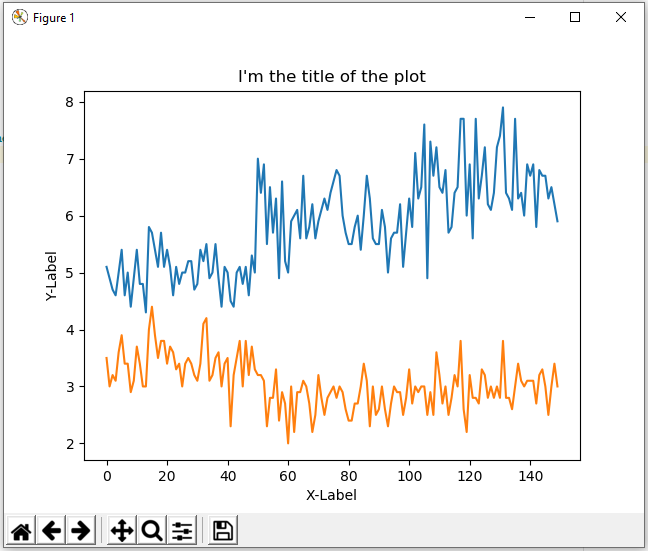
\includegraphics[width=1\textwidth]{images/MachineLearning/ml_sample_plot.png}
	\caption{Plot mit Titel und Achsenbeschriftungen}
	\label{ml:samples:ml_sample_plot}
\end{figure}


Eine weitere Darstellungsform k�nnte als Histogramm sein.

\randnotiz{Histogramm erzeugen}\lstinputlisting[language=Python]{chapters/advancedTopics/src/machinelearning/plothist.py}\label{defineplot1:lst:plothist}

Das erzeugte Histogramm sieht aus wie in Abbildung ~\ref{ml:samples:ml_sample_plothist}.

\begin{figure}[ht]
	\centering
	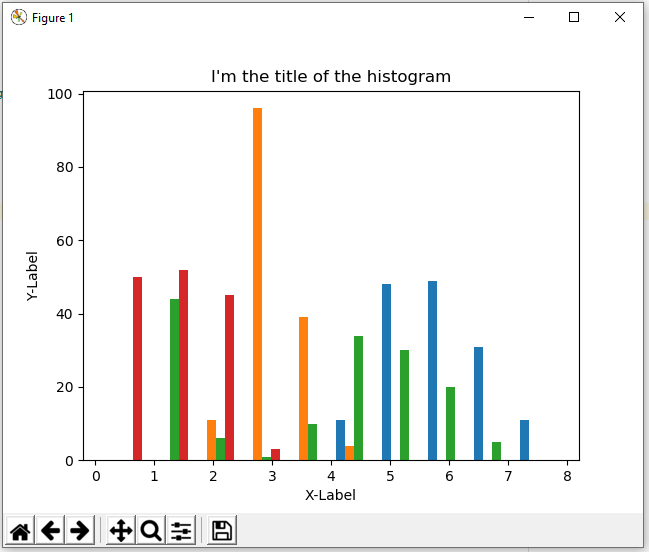
\includegraphics[width=1\textwidth]{images/MachineLearning/ml_sample_plothist.png}
	\caption{Histogram-Plot mit Titel und Achsenbeschriftungen}
	\label{ml:samples:ml_sample_plothist}
\end{figure}

F�r das Beispiel oben bietet sich au�erdem die Darstellung in einem Scatterplot an.

\randnotiz{Scatterplot erzeugen}\lstinputlisting[language=Python]{chapters/advancedTopics/src/machinelearning/plotscatter.py}\label{defineplot1:lst:plotscatter}

Der Code erzeugt einen Scatterplot wie in Abbildung ~\ref{ml:samples:ml_sample_plotscatter}.

\begin{figure}[ht]
	\centering
	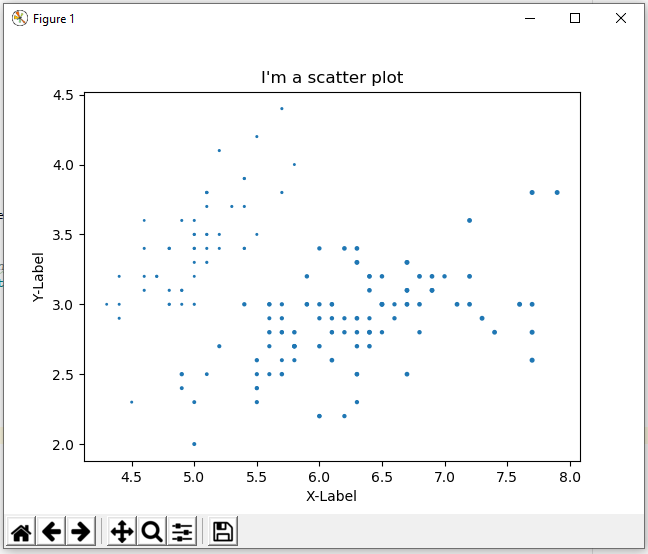
\includegraphics[width=1\textwidth]{images/MachineLearning/ml_sample_plotscatter.png}
	\caption{Scatter-Plot mit Titel und Achsenbeschriftungen}
	\label{ml:samples:ml_sample_plotscatter}
\end{figure}

\uebung
\aufgabe{MachineLearning/machinelearning_plots}

\subsection{Beispiel: knn-Klassifikation}\label{maschinelleslernen:knnklassifikation}
Der knn-Algorithmus ist einer der bekanntesten Algorithmus aus dem Bereich Klassifikation und wird daher hier als Codebeispiel dargestellt und erl�utert.

Folgende Imports\randnotiz{Imports} sind f�r dieses Beispiel n�tig:
\lstinputlisting[language=Python,firstline=4,lastline=11]{chapters/advancedTopics/src/machinelearning/knnsample.py}\label{knnsample:lst:knnsample4}

Anschlie�end k�nnen die Daten\randnotiz{Daten laden} geladen und die Spaltennamen definiert werden.
\lstinputlisting[language=Python,firstline=14,lastline=20]{chapters/advancedTopics/src/machinelearning/knnsample.py}\label{knnsample:lst:knnsample14}

Jetzt werden die Daten gelesen\randnotiz{Daten lesen und vorbereiten} und vorbereitet.
\lstinputlisting[language=Python,firstline=22,lastline=28]{chapters/advancedTopics/src/machinelearning/knnsample.py}\label{knnsample:lst:knnsample22}

Zur Berechnung m�ssen die Daten\randnotiz{Daten skalieren} skaliert werden.
\lstinputlisting[language=Python,firstline=33,lastline=37]{chapters/advancedTopics/src/machinelearning/knnsample.py}\label{knnsample:lst:knnsample33}

Nun kann der KNN-Algorithmus\randnotiz{Algorithmus anwenden} angewendet werden.
\lstinputlisting[language=Python,firstline=39,lastline=44]{chapters/advancedTopics/src/machinelearning/knnsample.py}\label{knnsample:lst:knnsample39}

Jetzt k�nnen wir die Daten-Matrix\randnotiz{Matrix ausgeben} ausgeben.
\lstinputlisting[language=Python,firstline=46,lastline=47]{chapters/advancedTopics/src/machinelearning/knnsample.py}\label{knnsample:lst:knnsample46}

Als Ausgabe wird Folgendes angezeigt
\begin{lstlisting}
[[ 9  0  0]
 [ 0 12  1]
 [ 0  1  7]]
\end{lstlisting} 
 
Zus�tzlich\randnotiz{Report ausgeben} kann ein Report angezeigt werden, welcher eine gute �bersicht �ber die klassifizierten Daten gibt.
\lstinputlisting[language=Python,firstline=48,lastline=49]{chapters/advancedTopics/src/machinelearning/knnsample.py}\label{knnsample:lst:knnsample49}

Die Ausgabe ist die folgende:
\begin{lstlisting} 
                  precision    recall  f1-score   support
 
     Iris-setosa       1.00      1.00      1.00         9
 Iris-versicolor       0.92      0.92      0.92        13
  Iris-virginica       0.88      0.88      0.88         8
 
       micro avg       0.93      0.93      0.93        30
       macro avg       0.93      0.93      0.93        30
    weighted avg       0.93      0.93      0.93        30
\end{lstlisting}



Um \randnotiz{Fehler ausgeben}ein abschlie�endes Bild �ber die Klassifikation zu erhalten k�nnen nun noch die Fehler ausgegeben werden.
\lstinputlisting[language=Python,firstline=51,lastline=61]{chapters/advancedTopics/src/machinelearning/knnsample.py}\label{knnsample:lst:knnsample51}


Aus\randnotiz{Fehler-Plot erzeugen} den berechneten Fehlern bei der Klassifikation kann nun noch ein Plot erzeugt werden.
\lstinputlisting[language=Python,firstline=64,lastline=72]{chapters/advancedTopics/src/machinelearning/knnsample.py}\label{knnsample:lst:knnsample64}

Der Plot zeigt sich wie in Abbildung ~\ref{ml:samples:plotknn}.

\begin{figure}[ht]
	\centering
	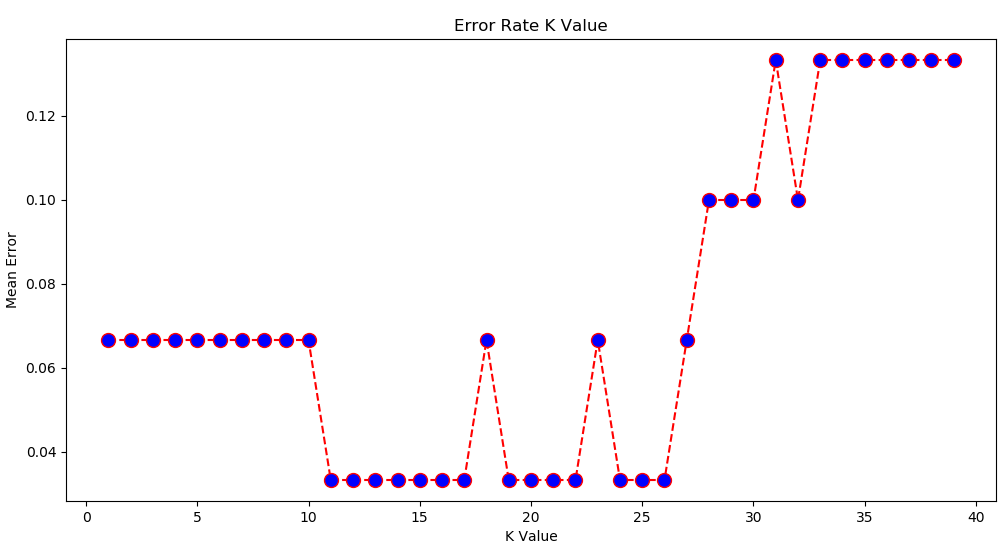
\includegraphics[width=1\textwidth]{images/MachineLearning/ml_knn_plot.png}
	\caption{Ergebnis-Plot der Fehler nach Ausf�hrung KNN}
	\label{ml:samples:plotknn}
\end{figure}

\uebung
\aufgabe{MachineLearning/machinelearning_knn}


\subsection{Beispiel: Naive Bayes}\label{maschinelleslernen:naivebayes}
Ein weiteres Beispiel aus dem Bereich Klassifikation im maschinellen Lernen ist der Naive Bayes Algorithmus.

Es \randnotiz{Importe}sind wieder einige Importe n�tig.
\lstinputlisting[language=Python,firstline=3,lastline=5]{chapters/advancedTopics/src/machinelearning/bayessample.py}\label{knnsample:lst:bayessample3}

Die \randnotiz{Daten laden}Beispieldaten m�ssen definiert werden.
\lstinputlisting[language=Python,firstline=7,lastline=11]{chapters/advancedTopics/src/machinelearning/bayessample.py}\label{knnsample:lst:bayessample7}

Nun \randnotiz{Modell erzeugen}kann das Modell erzeugt werden um mit den Daten zu trainieren. 
\lstinputlisting[language=Python,firstline=13,lastline=16]{chapters/advancedTopics/src/machinelearning/bayessample.py}\label{knnsample:lst:bayessample13}

Anschlie�end\randnotiz{Vorhersage} k�nnen die Daten vorhergesagt und die Ergebnisse angezeigt werden.
\lstinputlisting[language=Python,firstline=17,lastline=21]{chapters/advancedTopics/src/machinelearning/bayessample.py}\label{knnsample:lst:bayessample17}

Die Ausgabe dieser Vorhersage lautet:
\begin{lstlisting}
[3 4]
\end{lstlisting}


\uebung
\aufgabe{MachineLearning/machinelearning_bayes}


\subsection{Beispiel: Lineare Regression}\label{maschinelleslernen:linregress}
Beispiel aus dem Bereich Regression. Konkret wird hier eine lineare Regression dargestellt. 

Es \randnotiz{Importe}sind verschiedene Importe f�r n�tig. Die werden im ersten Schritt importiert.
\lstinputlisting[language=Python,firstline=1,lastline=5]{chapters/advancedTopics/src/machinelearning/linregress.py}\label{knnsample:lst:lingress1}

Daten \randnotiz{Daten laden}aus dem Datensatz \lstinline$boston$ auslesen und in \lstinline$numpy-array$ �berf�hren.
\lstinputlisting[language=Python,firstline=7,lastline=10]{chapters/advancedTopics/src/machinelearning/linregress.py}\label{knnsample:lst:lingress7}

Die \randnotiz{Berechnung durchf�hren}Berechnung der linearen Regression kann direkt aus dem Modul \lstinline$scipy$ erfolgen, es ist keine eigene Implementierung n�tig. Die Daten die analysiert werden sollen m�ssen entsprechend mitgegeben werden.
\lstinputlisting[language=Python,firstline=12,lastline=13]{chapters/advancedTopics/src/machinelearning/linregress.py}\label{knnsample:lst:lingress12}

Nun \randnotiz{Plot erzeugen}kann der Plot f�r die berechneten Werte erzeugt werden.
\lstinputlisting[language=Python,firstline=15,lastline=27]{chapters/advancedTopics/src/machinelearning/linregress.py}\label{knnsample:lst:lingress15}

Die Anzeige im Plot ist wie in Abbildung ~\ref{ml:samples:plotlinregress}.

\begin{figure}[ht]
	\centering
	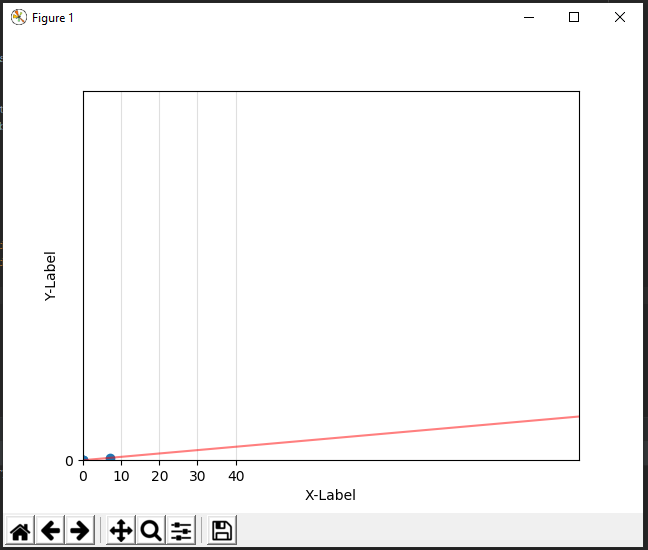
\includegraphics[width=0.9\textwidth]{images/MachineLearning/ml_linregress_plot.png}
	\caption{Ergebnis-Plot der linearen Regression}
	\label{ml:samples:plotlinregress}
\end{figure}

Somit haben wir nun auch eine lineare Regression erfolgreich durchgef�hrt.


\uebung
\aufgabe{MachineLearning/machinelearning_linregress}
% !TeX root = ../../pythonTutorial.tex

\section{Datenbanken}\label{database:einleitung}
In diesem Kapitel wird die Benutzung zweier verschiedener Datenbanksysteme, in der Programmiersprache Python, demonstriert. Zudem wird aufgef�hrt, wie eine Datenbank angelegt wird und wie die SQL-Befehle durchgef�hrt werden k�nnen.
\subsection{Relationale Datenbanken}\label{database:relationaldatabase}
Relationale Datenbanken, die bereits im dritten Semester in der Vorlesung \glqq Datenbanken\grqq  durchgenommen wurden, dienen zur elektronischen Speicherung von Daten. Im folgendem Kapitel wird das Einbinden von SQLite in eine Python-Anwendung genauer erl�utert.
\subsubsection{SQLite}\label{database:sqlite}
SQLite ist ein relationales Datenbankmanagementsystem, welches in einer C-Bibliothek enthalten ist. Anders als beispielsweise MySQL nutzt SQLite nicht das Client-Server-Model, sondern ist sp�ter im fertigen Programm lokal integriert. Eingesetzt wird SQLite sehr h�ufig in mobilen Applikationen. Diese speichern Nutzerdaten Lokal auf dem Ger�t. Im weiteren Verlauf des Kapitels wird das Einbinden von SQLite in eine Python-Anwendung erl�utert.

\textbf{Einbinden von SQLite}

Um SQL in einem Python-Projekt verwenden zu k�nnen, wird lediglich ein Import Statement ben�tigt.
\begin{lstlisting}[language=Python]
#import sqlite
import sqlite3
\end{lstlisting}\label{database:lst:importsqlite}
Anschlie�end muss eine neue Datenbank angelegt werden. Hierf�r kann die Methode \lstinline{connect()} verwendet werden. F�r diese Methode muss der �bergabeparameter aus einem String mit der Endung \glqq.db\grqq  �bergeben werden.
\begin{lstlisting}[language=Python]
#connect sqlite
connection = sqlite3.connect("beispiel.db")
\end{lstlisting}\label{database:lst:connect}

\kontrollfrage{
	\item[\kontroll] Wie wird in SQLite eine neue Datenbank angelegt?
}

Um einen String, welcher das SQL-Statement beinhaltet, in die Datenbank einzubinden, muss zus�tzlich ein Cursor angelegt werden.
\begin{lstlisting}[language=Python]
#connect curser anlegen
cursor = connection.cursor()
\end{lstlisting}\label{database:lst:cursor}
Auch muss, damit der Cursor richtig verwendet wird, dies innerhalb der Datenbankverbindung ausgef�hrt werden
Mit \lstinline{cursor.execute(sql_command)} wird eine Anfrage ausgef�hrt. Um den Cursor richtig zu verwenden, muss er innerhalb der Datenbankverbindung ausgef�hrt werden. 
\begin{lstlisting}[language=Python]
with connection:
	cur = connection.execute('sqlstatement')
\end{lstlisting}\label{database:lst:cursor}
Falls alle Tabellen angelegt und wie gewollt bef�llt wurden, k�nnen mit der Methode \lstinline{commit()} alle �nderungen an der Datenbank abgespeichert werden.
\begin{lstlisting}[language=Python]
#commit
connection.commit()
\end{lstlisting}\label{database:lst:commit}
Um die Verbindung zur Datenbank zu beenden wird die Methode \lstinline{close()} genutzt.
\begin{lstlisting}[language=Python]
#close
connection.close()
\end{lstlisting}\label{database:lst:close}

\textbf{Create bei SQLite} \randnotiz{CREATE}

In Folge dessen k�nnen nun einzelne Tabellen zur Datenbank hinzugef�gt werden. Dies kann umgesetzt werden, indem ein neuer \lstinline{sql_command} angelegt wird, welcher ein korrektes SQL-Kommando beinhalten muss.

\begin{lstlisting}[language=Python]
#create
sql_command = """
CREATE TABLE mitarbeiter( 
mitarbeiterid INTEGER PRIMARY KEY, 
vname VARCHAR(20), 
nname VARCHAR(30), 
geschlecht CHAR(1), 
beitritt DATE,
geburtstag DATE);"""
\end{lstlisting}\label{database:lst:create}
 
\textbf{Insert bei SQLite} \randnotiz{INSERT}

Um eine Tabelle im Anschluss zu bef�llen wie folgt bef�llt.
\begin{lstlisting}[language=Python]
#insert
sql_command = """INSERT INTO mitarbeiter
(mitarbeiterid, vname, nname, geschlecht, geburtstag)
VALUES (NULL, "Peter", "Maffay", "m", "30.08.1949");"""
\end{lstlisting}\label{database:lst:insert}

\textbf{Select bei SQLite} \randnotiz{SELECT}

Daten aus der SQLite Datenbank werden mit einem \lstinline{Select} Befehl ausgelesen.
Dieser erm�glicht es uns, einen oder mehrere Beitr�ge auszulesen. Mit dem SQL-Statment \lstinline{sql_command1} im Listing\ref{database:lst:select} werden alle Eintr�ge aus der Tabelle mitarbeiter ausgelesen.

\begin{lstlisting}[language=Python]
#select
sql_command1 = """SELECT * FROM mitarbeiter;"""
sql_command2 = """SELECT * FROM mitarbeiter 
WHERE mitarbeiterid = 1;"""

\end{lstlisting}\label{database:lst:select}

\textbf{Update bei SQLite} \randnotiz{UPDATE}

Um einen Eintrag im Nachhinein zu �ndern, kann durch den \lstinline{Update} Befehl ein oder mehrere bestimmte Eintr�ge ge�ndert werden. Im Listing wird der Vorname des Mitarbeiters mit der \lstinline{MitarbeiterId = 1} auf Peter gesetzt.
\begin{lstlisting}[language=Python]
#update
sql_command = """UPDATE mitarbeiter SET vname="Peter"
WHERE mitarbeiterid = 1;"""
\end{lstlisting}\label{database:lst:update}
\kontrollfrage{
\item[\kontroll] Welcher Befehl muss ausgef�hrt werden um einen bestehenden
 Eintrag zu �ndern?
}

\textbf{Delete bei SQLite} \randnotiz{DELETE}

Eine Tabelle oder einen bestimmten Mitarbeiter kann durch einen \lstinline{Delete} Befehl wieder entfernt werden. In folgendem Listing\ref{database:lst:delete} werden zwei M�glichkeiten Daten aus der Datenbank zu entfernen aufgezeigt.
\begin{lstlisting}[language=Python]
#delete
sql_command1 = """DELETE FROM mitarbeiter 
WHERE mitarbeiterid = 1;???
sql_command2 = """DELETE FROM mitarbeiter;???
\end{lstlisting}\label{database:lst:delete}

\subsection{NoSQL Datenbanken}\label{database:nosql}

NoSql steht f�r \glqq not only SQL\grqq{}. Hierbei wird SQL als Synonym f�r relationale Datenbanksysteme verwendet. Die Grundidee ist, dass nicht unbedingt aus alten Gewohnheiten heraus ein relationales Datenbanksystem gew�hlt wird. Vielmehr soll sich f�r ein Datenbanksystem entschieden werden, welches am Besten zum geplanten Projekt passt. Entstanden sind solche NoSQL Datenbanken unter anderem durch soziale Netzwerke. Hier m�ssen mehrere Millionen Daten sehr schnell gespeichert und abgerufen werden. Eine solche Masse an Anfragen stellt ganz neue Anforderung an Datenbanksysteme.\cite{mongodbtutorial}
Die wichtigsten Kategorien von NoSQL-Datenbanken sind Key-Value, spaltenorientierte, Value und dokumentenorientierte Datenbanken. Im folgendem Kapitel, wird das Einbinden der dokumentenbasierten NoSQL Datenbank MongoDB genauer beschrieben.\cite{mongodbtutorial}

\subsubsection{MongoDB}\label{database:mongodb}
MongoDB ist eine open-source dokumentenbasierte NoSQL-Datenbank, die unter anderem eine hohe Performance und automatische Skalierung bietet. Als \lstinline{record}
wird in MongoDB eine Datenstruktur (key/value) mit Name und den dazugeh�rigen Werten bezeichnet. Diese MongoDB Dokumente sind �hnlich zu den uns bekannten JSON-Objekten. Wie die Einbindung und die Benutzung einer MongoDB Datenbank umgesetzt wird, wird nachfolgend genauer erl�utert.

\textbf{Einbinden von MongoDB}

Um eine Verbindung mit MongoDB herzustellen, muss zun�chst die Python Distribution PyMongo installiert werden.
\begin{lstlisting}[language=Python]
#import mongodb
import pymongo
\end{lstlisting}\label{database:lst:importmongodb}
Anschlie�end muss mit mongod eine MongoDB Instanz gestartet werden.
\begin{lstlisting}[language=Python]
#mongod Instanz starten

$ mongod
client = MongoClient()
\end{lstlisting}\label{database:lst:client}
Im Anschluss darauf, muss ein MongoClient erstellt werden, welcher auf die laufende mongod Instanz zugreift und sich 
dabei mit dem Standart-Host und Standart-Port verbindet.
\begin{lstlisting}[language=Python]
#create client
from pymongo import MongoClient
client = MongoClient()
\end{lstlisting}\label{database:lst:client}
Host und Port k�nnen aber auch durch eines der folgenden Formate explizit spezifiziert werden.
\begin{lstlisting}[language=Python]
#Host Name und Passwort spezifizieren
client1 = MongoClient('localhost', 12345)
client2 = MongoClient('mongodb://localhost:12345/')
\end{lstlisting}\label{database:lst:host}
In PyMongo wird mit attribute style access auf die Datenbanken zugegriffen, da eine Instanz von MongoDB mehrere unabh�ngige Datenbanken unterst�tzt. Dabei k�nnen die beiden folgenden Formate verwendet
 werden.
\begin{lstlisting}[language=Python]
#Zugriff auf die Datenbank in zwei Varianten
db1 = client.test_database
db2 = client['test-database']
\end{lstlisting}\label{database:lst:databaseconnection}
Das �quivalent zu Tabellen in relationalen Datenbanken in MongoDB wird \glqq Connections\grqq{} genannt. Diese bestehen aus mehreren Dokumenten. Der Zugriff erfolgt genau wie bei einer SQL-Datenbank.
\begin{lstlisting}[language=Python]
#Zugriff auf Connections in zwei Varianten 
collection = db.test_collection
collection = db['test-collection']
\end{lstlisting}\label{database:lst:tableconnection}
Die oben genannten Dokumente (JSON-Style) sind die Repr�sentanten und Speicher der Daten in der Datenbank.
\begin{lstlisting}[language=Python]
#JSON
import datetime
test = {	"author": "Lukas",
"text": "Hallo",
"tags": ["hallo", "pymongo"]
"date": datetime.datetime.utcnow()}
\end{lstlisting}\label{database:lst:json}

\textbf{Insert und Delete bei MongoDB} \randnotiz{INSERT, DELETE}

Ein Dokument wird mit der Methode \lstinline{insert_one()} hinzugef�gt.
\begin{lstlisting}[language=Python]
#insert_one
test = db.test
test_id = test.insert_one(test).inserted_id
test_id
ObjectId('...')(Ausgabe)
\end{lstlisting}\label{database:lst:insertone}

Beim Einf�gen eines Dokuments wird diesem automatisch eine \lstinline{_id} zugewiesen, falls diese noch keine vorher bestimmte \lstinline{_id} hat. Die \lstinline{_id} muss einzigartig in einer Collection sein. Nachdem das Dokument hinzugef�gt wurde, wird eine Test Collection erstellt. Mit Hilfe der Ausgabe einer Liste aller Collections wird dies best�tigt. 
\begin{lstlisting}[language=Python]
#collection_names
db.collection_names(include_system_collections=False)
\end{lstlisting}\label{database:lst:collectionnames}
Um ein bereits hinzugef�gtes Dokument zu l�schen wird die Methode \lstinline{delete_one()} verwendet.

\textbf{Select bei MongoDB} \randnotiz{SELECT}

Mit der Methode \lstinline{find_one()}\ref{database:lst:findone} kann auf bestimmte oder das erste (kein Parameter) Dokument einer Collection zugegriffen werden.
\begin{lstlisting}[language=Python]
#find_one mit autor
test.find_one({"author": "Lukas"})
\end{lstlisting}\label{database:lst:findone}
Mit Hilfe der \lstinline{_id} kann auch auf einzelne Dokumente zugegriffen werden.
\begin{lstlisting}[language=Python]
#find_one mit id
test.find_one({?_id?: test_id})
\end{lstlisting}\label{database:lst:findone}


\kontrollfrage{
	\item[\kontroll] Wof�r wird bei MongoDB die Methode find() verwendet?
}

\textbf{Update bei MongoDB} \randnotiz{UPDATE}

Um einem Dokument neue Parameter geben zu k�nnen, kann die Methode 
\lstinline{update_one(altes Dokument, neues Dokument)} genutzt werden. Das neue Dokument muss den Operator \lstinline{$set} enthalten. 
\begin{lstlisting}[language=Python]
#update
newvalue { "$set": { "author": "Lukas" } }
\end{lstlisting}\label{database:lst:update}
Die Methoden \lstinline{insert_one()} und \lstinline{find_one()} k�nnen in abge�nderter Form auch f�r mehrere Dokumente genutzt werden. 
Mehrere Dokumente werden mit \lstinline{insert_many()} hinzugef�gt.

Einen Zugriff auf mehrere Dokumente wird mit \lstinline{find()} umgesetzt.
Die Anzahl der Dokumente wird in unserem Fall mit \lstinline{test.count_documents()} ausgelesen.
Mit \lstinline{.sort} werden Ergebnisse nach verschiedenen Parametern sortiert.
In Listing\ref{database:lst:createindex} wird ein neuer Index erstellt.
\begin{lstlisting}[language=Python]
#Create Index
result = db.profiles.create_index(
[('user_id',pymongo.ASCENDING)],unique=True)
\end{lstlisting}\label{database:lst:createindex}
Dies hat zur Folge, dass nun \lstinline{_id}und \lstinline{user_id} existieren, welche einzigartig sein m�ssen.
Zuletzt wird die Verbindung mit der Datenbank unterbrochen.
\begin{lstlisting}[language=Python]
#close
client.close
\end{lstlisting}\label{database:lst:close}

\kontrollfrage{
	\item[\kontroll] Wof�r wird die Methode count\_documents({}) verwendet?
}

\uebung

\aufgabe{database01}
\aufgabe{database02}

% !TeX root = ../pythonTutorial.tex
\section{Nebenl�ufigkeit}
\label{nebenl�ufigkeit:section:nebenl�ufigkeit}

Mit Nebenl�ufigkeit ist eine Eigenschaft von zwei oder mehr Aktivit�ten gemeint.
Eine beliebige Anzahl an Aktivit�ten wird als nebenl�ufig bezeichnet, wenn die
Reihenfolge der Ausf�hrung der einzelnen Aktivit�ten irrelevant f�r das Ergebnis ist.
Hierbei ist auf den Unterschied zwischen Nebenl�ufigkeit und Parallelit�t zu achten.
W�hrend Nebenl�ufigkeit eine Eigenschaft darstellt, ist Parallelit�t eine m�gliche
Herangehensweise an das Ausf�hren von nebenl�ufigen Aktivit�ten (vgl. \cite{exppypro}).

Im folgenden Kapitel wird beschrieben, wie in Python durch Threads und Prozesse
nebenl�ufige Programmierung realisiert werden kann.
Python unterscheidet sich in Bezug auf Parallelit�t stark von anderen Programmiersprachen.
In Abschnitt \ref{parallelit�t_in_python:subsection:parallelit�t_in_python} wird auf diesen
Unterschied eingegangen.
Anschlie�end wird in Abschnitt \ref{threads:subsection:threads} beschrieben, wie in Python Nebenl�ufigkeit
durch Threads realisiert werden kann.
Neben der Erzeugung von Threads werden Synchronisations- und Steuerungsmechanismen besprochen.
Nachdem nun Nebenl�ufigkeit durch Threads erreicht wurde, wird sich in Abschnitt
\ref{prozesse:subsection:prozesse}
auf Prozesse bezogen.

% !TeX root = ../../pythonTutorial.tex
\subsection{Parallelit�t in Python}
\label{parallelit�t_in_python:subsection:parallelit�t_in_python}

In der Referenzimplementierung CPython des Python-Interpreters existiert ein Konstrukt,
welches eine echte parallele Ausf�hrung von Python-Code verhindert.
Bei diesem Konstrukt handelt es sich um das sogenannte Global-Interpreter-Lock, oder kurz GIL.
F�r die Verwendung eine GILs in Python sprechen mehrere Punkte.
Python wurde so entworfen, dass es leicht zu verwenden ist, um den
Entwicklungsprozess zu beschleunigen.
Ein GIL verhindert, dass sich mehrere Threads gleichzeitig in der Ausf�hrung befinden k�nnen,
was die Entwicklung von Multithreaded-Programmen erheblich erleichtert.
Weiterhin wurde der Funktionsumfang von Python durch viele in C geschriebene Erweiterungen erg�nzt.
Um Inkonsistenzen zu verhindern, ben�tigen diese C-Erweiterungen eine threadsichere
Speicherverwaltung, die durch das GIL garantiert ist.
Die Verwendung des GILs erleichtert auch die Integration von nicht threadsicheren C-Bibliotheken.
Da das Einbinden von C-Bibliotheken durch das GIL leicht zu realisieren ist, existieren
viele Erweiterungen zu Python, die zur weiten Verbreitung von Python f�hrten.

Durch die Verwendung des GILs ist eine parallele Programmierung in Python
allerdings nicht g�nzlich ausgeschlossen.
Lediglich Aufgaben, die CPU-gebunden sind, sind hierdurch betroffen.
I/O-gebundene Aufgaben, wie zum Beispiel die Anfragea von Daten aus einer Datenbank, oder
die Abfrage von Benutzereingaben, k�nnen auch trotz des GILs parallel ausgef�hrt werden.
Durch die Verwendung von mehreren Prozessen ist es auch m�glich, parallele
Ausf�hrung von Python-Code zu erreichen.
Dies funktioniert, da jeder Python-Prozess seinen eignen Python-Interpreter und somit
auch ein eigenes GIL besitzt.

% !TeX root = ../../pythonTutorial.tex
\subsection{Threads}
\label{threads:subsection:threads}

In Python werden zwei APIs zur Verwendung von Threads angeboten, die Low-Level
API aus dem \_thread-Modul und die Higher-Level API aud dem threading-Modul.
Es wird sich an dieser Stelle auf das threading-Modul beschr�nkt, da es intern auf
dem \_thread-Modul basiert und eine Schnittstelle anbietet, die das Programmieren
von Multithreaded-Programmen erleichert.
Diese Schnittstelle ist an der Thread-Schnittstelle von Java angelehnt und sollte daher f�r
Java-Entwickler leicht zu verwenden sein.
Allerdings gibt es einige Unterschiede zwischen dem Python-Modul und der entsprechenden
Implementierung in Java.
So sind Bedingungsvariablen und Locks seperate Objekte in Python und es ist auch
nur eine Teilmenge des Verhaltens eines Java-Threads in Python verf�gbar.
Ein Python-Thread kennt keine Priorit�ten und Thread-Gruppen und er kann nicht zerst�rt,
gestopped, angehalten, fortgesetzt oder unterbrochen werden.
Soweit vorhanden sind die statischen Methoden aus der Java-Thread-Klasse auf Modul-Ebene
in Python implementiert.

\subsubsection{Thread Objekte}
\label{threads:subsubsection:thread_objekte}

Es gibt zwei M�glichkeiten einen Thread zu erzeugen. Entweder wird dem Konstruktor ein
aufrufbares Objekt �bergeben,

\label{threads:lst:thread_erzeugung_callable}
\lstinputlisting[language=Python,linerange={1-2,6-12}]{chapters/nebenlaufigkeit/src/thread_erzeugung.py}

oder die \lstinline$run()$-Methode wird in einer von \lstinline$Thread$ abgeleiteten Klasse �berschrieben.

\label{threads:lst:thread_erzeugung_subclass}
\lstinputlisting[language=Python,linerange={1-2,14-21}]{chapters/nebenlaufigkeit/src/thread_erzeugung.py}

Der Konstruktor  der \lstinline$Thread$-Klasse bietet noch weitere Parameter an:
\begin{itemize}
    \item \lstinline$group$ sollte immer \lstinline$None$ sein.
    Es ist aktuell reserviert f�r sp�tere Erweiterungen.
    \item \lstinline$name$ setzt den Namen des Threads.
    \item \lstinline$args$ ist ein Tupel aus Parametern f�r das mit \lstinline$target$ definierte
    aufrufbare Objekt.
    \item \lstinline$kwargs$ ist ein Dictionary aus Schl�sselwort-Parametern f�r \lstinline$target$.
    \item \lstinline$deamon$ setzt die D�mon-Eigenschaft des Threads.
\end{itemize}

Es ist anzumerken, dass ein \lstinline$Thread$-Objekt bei seiner Erzeugung noch nicht gestartet wird.
Hierzu muss explizit die \lstinline$start()$-Methode aufgerufen werden.
Wurde ein Thread gestartet, wird er als \glqq lebendig\grqq{} angesehen. 
Dies bleibt er solange, bis seine \lstinline$run()$-Methode verlassen wurde.
Hierbei macht es keinen Unterschied, ob sie regul�r verlassen wurde oder Aufgrund einer Exception.
Der aktuelle Status eines Threads kann mittels der \lstinline$is_alive()$-Methode abgefragt werden.
Soll auf das Beenden eines anderen Threads gewartet werden, so kann seine
\lstinline$join()$-Methode aufgerufen werden. 
Hiermit wird der aufrufende Thread blockiert, bis der andere beendet ist.
Die \lstinline$join$-Methode nimmt einen optionalen Parameter des Typen \lstinline$float$ entgegen,
der als Timeout in Sekunden dient.
Wird ein Timeout angegeben, ist es wichtig, dass nach dem \lstinline$join()$-Aufruf die Methode 
\lstinline$is_alive()$ aufgerufen wird.
Da \lstinline$join()$ immer \lstinline$None$ zur�ckgibt, ist es ansonsten nicht m�glich, zu wissen, ob
der Thread tats�chlich beendet wurde, oder nur der Timeout abgelaufen ist.

\kontrollfrage{
\item[\kontroll] Wie kann auf das Ende der Ausf�hrung eines Threads gewartet werden?
}

Jeder Thread besitzt einen Namen, der initial �ber den Konstruktor oder direkt �ber das
\lstinline$name$-Attribut gesetzt werden kann. 
Threads k�nnen als D�mon gekennzeichnet werden.
Sobald nur noch D�mon-Threads aktiv sind, wird das Python-Programm beendet.
Die D�mon-Eigenschaft kann initial �ber den Konstruktor gesetzt werden.
Wird kein Wert �bergeben, �bernimmt der Thread standardm��ig den Wert des erzeugenden Threads.
�ber das \lstinline$deamon$-Attribut eines Threads kann die Eigenschaft abgefragt und gesetzt werden.
Hierbei ist es wichtig, dass die Eigenschaft immer vor dem Aufruf der \lstinline$start()$-Methode
gesetzt wird.
Wird sie nach dem Starten des Threads ge�ndert, so wird ein \lstinline$RuntimeError$ geworfen.

\warning{
	D�mon-Threads werden sofort beendet, wenn keine normalen Threads mehr aktiv sind.
	Das hei�t, dass ihre Ressourcen, wie zum Beispiel ge�ffnete Dateien oder Datenbanktransaktionen,
	gegebenenfalls nicht ordentlich freigegeben werden.
	Um dies zu verhindern, sollten die betroffenen Threads nicht die D�mon-Eigenschaft besitzen und
	es sollten geeignete Signalisierungsmechanismen eingesetzt werden (siehe Abschnitt
	\ref{threads:subsubsection:thread-kommunikation}).
}

\uebung
\aufgabe{nebenlaufigkeit01}
\aufgabe{nebenlaufigkeit02}


\subsubsection{Synchronisation}
\label{threads:subsubsection:synchronisation}

Die meisten Anwendungen, in denen mehrere Threads zum Einsatz kommen, erfordern einen
Mechanismus, der die Zugriffe der einzelnen Threads auf gewisse Daten synchronisiert.
Hierdurch wird unteranderem vermieden, dass auf invaliden Datens�tzen gearbeitet wird, oder ein
Datenupdate verloren geht.
Im Folgenden wird ein Beispiel betrachtet, bei dem es zu Fehlern aufgrund von fehlender
Synchronisationsmechanismen kommt.
Es werden anschlie�end neue Konstrukte eingef�hrt, die die Fehler beheben werden.

Betrachtet wird nun die folgende \hyperref[threads:lst:counter_example]{\lstinline$Counter$-Klasse}.
Sie besitzt das Attribut \lstinline$count$, welches durch Aufruf von \lstinline$increment()$
in Einerschritten erh�ht wird. 

\label{threads:lst:counter_example}
\lstinputlisting[language=Python,linerange={1-3,7-13}]{chapters/nebenlaufigkeit/src/synchronisation_fehler.py}

Es ist weiterhin die \hyperref[threads:lst:incrementer_thread]{\lstinline$IncrementerThread$-Klasse}
gegeben, welche bei der Initialisierung ein \lstinline$Counter$-Objekt erwartet.
Dieser Thread ruft eine Millionen mal die \lstinline$increment()$-Methode des \lstinline$Counters$
auf und beendet sich anschlie�end.

\label{threads:lst:incrementer_thread}
\lstinputlisting[language=Python,linerange={1-3,15-23}]{chapters/nebenlaufigkeit/src/synchronisation_fehler.py}

F�r dieses Beispiel werden nun 10 \lstinline$IncrementerThreads$ erzeugt und gestartet.
Anschlie�end wird auf ihre Terminierung gewartet und dann der Wert des \lstinline$count$-Attributs des
\lstinline$Counters$ ausgegeben:

\label{threads:lst:example_no_locks}
\lstinputlisting[language=Python,linerange={1-3,25-36}]{chapters/nebenlaufigkeit/src/synchronisation_fehler.py}

\kontrollfrage{
\item[\kontroll] Welche Ausgabe w�rde erwartet werden, wenn 10 Threads den Counter eine Millionen
mal inkrementieren?
}

Dieser Programmcode w�rde vermuten lassen, dass bei jeder Ausf�hrung der Wert 10000000 ausgegeben
wird, da jeder der 10 Threads den \lstinline$Counter$ eine Millionen mal inkrementiert.
Erstaunlicherweise werden allerdings bei mehrmaliger Ausf�hrung unterschiedliche Werte ausgegeben.
Diese k�nnen zum Beispiel wie folgt aussehen:

\label{threads:lst:beispiel_ausgabe}
\begin{lstlisting}
# M�gliche Ausgaben:
5237496
3561559
4089438
4526494
\end{lstlisting}

Dieses Ph�nomen l�sst sich so erkl�ren, dass die Operation in \lstinline$increment()$ nicht atomar ist.
Genau genommen werden in ihr drei Operationen, eine lesende, eine addierende und eine schreibende,
ausgef�hrt.
Somit kann es vorkommen, dass zum Beispiel der erste Thread den aktuellen \lstinline$count$-Wert liest
und dann die aktive Ausf�hrung an einen anderen Thread abgeben muss.
Dieser zweite Thread liest nun den selben \lstinline$count$-Wert wie der erste Thread, inkrementiert ihn
und schreibt den neuen Wert zur�ck in das Attribut.
Nun wechselt die aktive Ausf�hrung zur�ck zum ersten Thread, welcher noch den alten
\lstinline$count$-Wert gelesen hat.
Dieser alte Wert wird nun erneut inkrementiert und zur�ckgeschrieben. 
Somit wurde der \lstinline$Counter$ effektiv nicht zweimal, sondern nur einmal inkrementiert.
Um dieses Verhalten zu verhindern, muss sichergestellt werden, dass die drei einzelnen Operationen
atomar ausgef�hrt werden, sprich, dass sie entweder ganz oder gar nicht ausgef�hrt werden.

Als unterste Synchronisationsebene bietet Python die Klasse \lstinline$Lock$ an.
\randnotiz{Locks}
Ein Objekt dieser Klasse befindet sich immer in einem von zwei Zust�nden, es ist entweder offen
oder geschlossen.
Nach der Initialisierung befindet es sich zuerst im ge�ffneten Zustand.
Ein \lstinline$Lock$-Objekt stellt die beiden Methoden \lstinline$acquire()$ und \lstinline$release()$ zur
Verf�gung.
Wird \lstinline$acquire()$ auf einem offenen \lstinline$Lock$ aufgerufen, so begibt sich das \lstinline$Lock$
in den geschlossenen Zustand und die Methode kehrt sofort zur�ck.
Sollte die \lstinline$aquire()$-Methode aufgerufen werden, wenn sich das \lstinline$Lock$ im
geschlossenen Zustand befindet, so blockiert sie solange, bis \lstinline$release()$ in einem anderen Thread
aufgerufen wird und somit den Zustand des \lstinline$Locks$ wieder zu ge�ffnet �ndert.
Die blockierte \lstinline$aquire()$-Methode schlie�t dann das \lstinline$Lock$ wieder und kehrt zur�ck.
Wird auf einem offenen \lstinline$Lock$ die \lstinline$release()$-Methode aufgerufen, so wird ein
\lstinline$RuntimeError$ geworfen.
Falls mehrere Threads durch \lstinline$aquire()$ blockiert werden, wird nur ein Thread fortgesetzt, sobald
\lstinline$release()$ aufgerufen wurde.
Welcher der blockierten Threads fortgesetzt wird, ist hierbei nicht definiert.

Wurde \lstinline$aquire()$ aufgerufen, sollte garantiert sein, dass auch \lstinline$release()$
aufgerufen wird.
Wird eine \lstinline$Exception$ geworfen, kann dies allerdings nicht immer garantiert sein.
Aus diesem Grund wird empfohlen, den durch das \lstinline$Lock$ gesch�tzten Programmcode in
einen \lstinline$try$-Block zu schreiben und den Aufruf von \lstinline$release()$ in den
\lstinline$finally$-Block zu schreiben:

\label{threads:lst:try_aquire_lock}
\lstinputlisting[language=Python,linerange={1-2,7-12}]{chapters/nebenlaufigkeit/src/lock_aquire_release.py}

Das Gleiche kann mit dem \lstinline$with$-Statement erreicht werden, da die \lstinline$Lock$-Klasse
das Context-Management-Protokoll unterst�tzt.
Hierbei werden die beiden Methoden \lstinline$aquire()$ und \lstinline$release()$ automatisch aufgerufen:

\label{threads:lst:with_aquire_lock}
\lstinputlisting[language=Python,linerange={1-2,13-15}]{chapters/nebenlaufigkeit/src/lock_aquire_release.py}

Ist es nicht gew�nscht, dass \lstinline$aquire()$ blockiert, wenn sie mehrmals aufgerufen wird, ohne 
dass das \lstinline$Lock$ freigegeben wurde, so kann ihr auch der optionale Parameter
\lstinline$blocking=False$ �bergegeben werden. 
In diesem Fall kehrt \lstinline$aquire()$ sofort zur�ck, egal in welchem Zustand sich das \lstinline$Lock$
befindet.
Es muss nun der R�ckgabewert von \lstinline$aquire()$ betrachtet werden, um zu erfahren, ob das 
\lstinline$Lock$ offen oder geschlossen ist.
Ist das \lstinline$Lock$ bereits geschlossen, wird der Wert \lstinline$False$ zur�ckgegeben.
Andernfalls wird \lstinline$True$ zur�ckgegeben und das \lstinline$Lock$ �ndert seinen Zustand zu
geschlossen.
Weiterhin ist es m�glich, einen Timeout mittels des optionalen Parametes \lstinline$timeout$ zu 
spezifizieren.
Hierbei kann eine beliebige Zeit in Sekunden als \lstinline$float$ Wert angegeben werden.
In diesem Fall blockiert \lstinline$aquire()$ maximale die spezifizierte Zeit.
Wurde in dieser Zeit das \lstinline$Lock$ erlangt, so gibt \lstinline$aquire()$ \lstinline$True$ zur�ck,
andernfalls \lstinline$False$.
Die Angabe eines Timeouts ist nur erlaubt, wenn der Parameter \lstinline$blocking$ den Wert
\lstinline$True$ besitzt.

\uebung
\aufgabe{nebenlaufigkeit03}
\aufgabe{nebenlaufigkeit04}

Um das Problem aus Aufgabe \ref{nebenlaufigkeit04} zu l�sen, bietet Python eine weitere M�glichkeit
zur Synchronisation an.
\randnotiz{Reentrant Locks}
Hierbei handelt es sich um die \lstinline$RLock$-Klasse.
Das \lstinline$R$ steht f�r \lstinline$reentrant$, was Wiedereintritt bedeutet.
Im Gegensatz zu Objekten der \lstinline$Lock$-Klasse, die nie einem Thread zugeordnet werden, werden
Objekte der \lstinline$RLock$-Klasse an den Thread gebunden, der zuerst die \lstinline$aquire()$-Methode
aufruft.
Neben den beiden Zust�nden, die die \lstinline$Lock$-Klasse besitzt, merkt sich die \lstinline$RLock$-Klasse
nun auch, wie oft die \lstinline$aquire()$-Methode aufgerufen wurde.
Beim ersten Aufruf von \lstinline$aquire()$ merkt sich das \lstinline$RLock$-Objekt, welcher Thread die
Methode aufgerufen hat und setzt einen internen Z�hler auf 1.
Bei jedem weiteren Aufruf von \lstinline$aquire()$ desselben Threads wird der Z�hler inkrementiert.
Wird \lstinline$release()$ aufgerufen, so wird der Z�hler wieder dekrementiert.
Das \lstinline$RLock$ ist erst dann wieder offen, wenn die Methode \lstinline$release()$ genau so oft
aufgerufen wurde, wie \lstinline$aquire()$, und der interne Z�hler wieder auf 0 steht.
Ruft ein zweiter Thread die \lstinline$aquire()$-Methode auf, w�hrend der erste Thread das
\lstinline$RLock$ besitzt, so muss er warten, bis der Z�hler wieder auf 0 steht.
Es ist nun also m�glich, einen gewissen Codeabschnitt auch rekursiv vor konkurrierenden Zugriffen 
zu sch�tzen.
Wie auch schon beim \lstinline$Lock$, k�nnen der \lstinline$aquire()$-Methode des \lstinline$RLocks$ 
die beiden optionalen Paramter \lstinline$blocking$ und \lstinline$timeout$ �bergegeben werden.

\uebung
\aufgabe{nebenlaufigkeit05}

Im Folgenden wird das Beispiel mit dem \lstinline$Counter$ und dem \lstinline$Incrementer-$
\lstinline$Thread$ etwas angepasst.
Der \lstinline$IncrementerThread$ soll nun den \lstinline$Counter$ wieder nur um eins erh�hen.
Weiterhin wird dem \lstinline$IncrementerThread$ ein Wert �bergeben, mit dem gesteuert wird,
wann der Thread den \lstinline$Counter$ erh�ht. Den 10 erstellten \lstinline$IncrementerThreads$ 
wird nun eine Zahl von 0 bis 9 �bergeben. Der \lstinline$Counter$ soll von den einzelnen Threads immer
nur dann erh�ht werden, wenn der aktuelle Wert des \lstinline$Counters$ auf die Ziffer endet, die dem
Thread bei der Erzeugung �bergeben wurde.
Demnach m�ssen die \lstinline$IncrementerThreads$ auf einen bestimmten geteilten Zustand warten,
bevor sie \lstinline$increment()$ aufrufen d�rfen.
\randnotiz{Condition-Variable}
F�r einen solchen Anwendungsfall stellt Python die \lstinline$Condition$-Klasse zur Verf�gung.
Der Mechanismus, der hierdurch implementiert wird, ist allgemein als Condition Variable
(deutch Bedingungsvariable) bekannt.
Objekte der \lstinline$Condition$-Klasse sind immer einem \lstinline$Lock$- oder einem
\lstinline$RLock$-Objekt zugeordnet.
Dieses kann dem Konstruktor eines \lstinline$Condition$-Objekts �bergeben werden.
Wird kein Lock-Objekt �bergeben, erzeugt der Konstruktor ein neues.
Das so erzeugte \lstinline$Condition$-Objekt kann nun �berall wie das Lock-Objekt
verwendet werden, das Lock-Objekt muss nicht weiterhin zus�tzlich verwaltet werden.
Es kann nun also das \lstinline$RLock$ aus der \lstinline$Counter$-Klasse gegen eine Condition Variable
ausgetauscht werden.
Die neue \hyperref[threads:lst:counter_condition_variable_example]{\lstinline$Counter$-Klasse} sieht
dann wie folgt aus:

\label{threads:lst:counter_condition_variable_example}
\lstinputlisting[language=Python,linerange={1-2,6-18}]{chapters/nebenlaufigkeit/src/condition_variable.py}

Eine Condition Variable kann also wie ein einfaches Lock verwendet werden.
Die \lstinline$aquire()$- und \lstinline$release()$-Methoden verhalten sich hierbei wie die des hinterlegten
Lock-Objekts.
Dar�ber hinaus bietet die \lstinline$Condition$-Klasse noch weitere Methoden an.
Diese Methoden d�rfen nur aufgerufen werden, wenn zuvor \lstinline$aquire()$ aufgerufen wurde.
Wurde von einem Thread \lstinline$aquire()$ aufgerufen, aber der aktuelle geteilte Zustand
nicht den gew�nschten Bedingungen entspricht, so wird \lstinline$wait()$ aufgerufen.
Die \lstinline$wait()$-Methode gibt das Lock wieder frei und blockiert den Thread, bis er
aufgeweckt wird.
Ein Thread wird durch Aufruf der \lstinline$notify()$- oder der \lstinline$notifiy_all()$
-Methode aufgeweckt.
Diese Methoden sollten immer dann aufgerufen werden, wenn der geteilte Zustand von einem Thread 
ge�ndert wurde.
Sobald ein Thread aufgeweckt wurde, fordert \lstinline$wait()$ wieder das Schloss an und kehrt
dann zur�ck.
Nachdem \lstinline$wait()$ zur�ckgekehrt ist, sollten die Bedingungen an den geteilten Zustand auf 
jeden Fall wieder gepr�ft werden, da eine unbestimmte Zeit zwischen dem Aufruf von \lstinline$notify()$
oder \lstinline$notify_all()$ und dem Zur�ckkehren von \lstinline$wait()$ vergehen kann.
Weiterhin ist es m�glich, \lstinline$wait()$ den optionalen Parameter \lstinline$timeout$ mitzugeben.
L�uft diese Zeit ab, bevor ein anderer Thread \lstinline$notify()$ oder \lstinline$notify_all()$ aufruft,
kehrt \lstinline$wait()$ mit dem R�ckgabewert \lstinline$False$ zur�ck.

\tip{
Um die Entscheidung zwischen \lstinline$notify()$ und \lstinline$notify_all()$ zu erleichtern, sollte die Frage
gestellt werden, ob die �nderung des geteilten Zustands f�r nur einen Thread oder mehrere Threads
interessant ist.
}

Durch einen Aufruf von \lstinline$notify_all()$ werden alle Threads, die \lstinline$wait()$ auf dem
entsprechenden \lstinline$Condition$-Objekt aufgerufen haben, aufgeweckt.
Mit \lstinline$notify()$ wird nur ein Thread aufgeweckt.
Es kann ein optionaler Parameter \lstinline$n$ an \lstinline$notify()$ �bergeben werden, der angibt, wie
viele Threads aufgeweckt werden sollen.

\warning{
	Durch den Aufruf von \lstinline$notify()$ und \lstinline$notify_all()$ wird das Lock nicht freigegeben.
	Das hei�t, dass Threads, die \lstinline$wait()$ aufgerufen haben, erst dann wieder aufwachen, wenn
	der Thread, der \lstinline$notify()$ oder \lstinline$notify_all()$ aufgerufen hat das Lock wieder 
	explizit frei gibt.
}

\kontrollfrage{
\item[\kontroll] Ist es f�r das \lstinline$Counter$ und \lstinline$IncrementerThread$ Beispiel ausreichend,
\lstinline$notify()$ aufzurufen?
}

Das \lstinline$Counter$ und \lstinline$IncrementerThread$ Beispiel w�rde nicht funktionieren, wenn 
immer nur ein beliebiger Thread geweckt wird. 
Wird der \lstinline$Counter$ inkrementiert, muss \lstinline$notify_all()$ aufgerufen werden,
um einen Deadlock zu vermeiden.
Dies liegt daran, das immer nur genau ein wartender Thread fortschreiten kann und es ist nicht
garantiert werden kann, dass genau dieser Thread aufgeweckt wird.

Wie das generische \hyperref[threads:lst:producer_consumer]{Producer-Consumer-Pattern}
mithilfe von Condition Variablen implementiert werden kann, ist im folgenden Listing
gezeigt (vgl. \cite{pythondokuthreads}).
Die Consumer warten so lange, bis der geteilte Zustand der Bedingung entspricht.
In diesem Fall hei�t das, dass mindestens ein Element verf�gbar ist.
Sobald ein Producer ein Element erstellt hat, ruft er \lstinline$notify()$ auf.
Somit wird genau ein Consumer aufgeweckt.
In diesem Beispiel reicht es vollkommen aus, nur einen Consumer aufzuwecken.

\label{threads:lst:producer_consumer}
\lstinputlisting[language=Python,linerange={1-2,23-33}]{chapters/nebenlaufigkeit/src/producer_consumer.py}

Der Consumer ruft \lstinline$wait()$ innerhalb der \lstinline$while$-Schleife auf und pr�ft
jedes mal seine Bedingung.
Dies ist notwendig, da sich der Zustand zwischen dem Aufruf von \lstinline$notify()$ und dem 
Zur�ckkehren von \lstinline$wait()$ erneut �ndern kann. 
Diese Problematik ist in der Multithreaded-Programmierung inh�rent.
Die \lstinline$Condition$-Klasse bietet neben \lstinline$wait()$ eine weitere Methode an, die das Testen
der Bedingung automatisieren kann.
Bei dieser Methode handelt es sich um \lstinline$wait_for()$.
Ihr Paramater \lstinline$predicate$ nimmt ein Callable-Objekt entgegen, welches einen boolischen Wert
zur�ck gibt.
Es kann zudem ein Timeout angegeben werden, der sich wie bei \lstinline$wait()$ verh�lt.
Wird \lstinline$wait_for()$ verwendet, �ndert sich das
\hyperref[threads:lst:producer_consumer_wait_for]{Producer-Consumer-Pattern Beispiel}
folgender Ma�en (vgl. \cite{pythondokuthreads}):

\label{threads:lst:producer_consumer_wait_for}
\lstinputlisting[language=Python,linerange={1-2,34-38}]{chapters/nebenlaufigkeit/src/producer_consumer.py}

\uebung
\aufgabe{nebenlaufigkeit06}

Eine weitere Problematik, die bei der Multithreaded-Programmierung vorkommt, ist das Sch�tzen
einer Ressource mit einer begrenzten Kapazit�t.
Als Beispiel aus dem Alltag dient hierf�r ein Parkhaus, welches nur eine begrenzte Anzahl an
Parkpl�tzen besitzt.
Es d�rfen sich immer nur maximal so viele Autos im Parkhaus befinden, wie Parkpl�tze vorhanden sind.
Die Klasse \hyperref[threads:lst:parkhaus]{\lstinline$CarPark$} simuliert ein Parkhaus und verwendet
eine Condition Variable, um sich vor konkurrierenden Zugriffen zu sch�tzen.

\label{threads:lst:parkhaus}
\lstinputlisting[language=Python,linerange={1-2,8-32}]{chapters/nebenlaufigkeit/src/parkhaus.py}

Ein Auto, dass zuerst eine gewisse Zeit umher f�hrt, bevor es eine zuf�llige Zeit parkt, wird durch die
Klasse \hyperref[threads:lst:auto]{\lstinline$Car$} simuliert.
Um eine zuf�llige Zeit im Intervall von \lstinline$x$ bis \lstinline$y$ zu schlafen wird hier die
\lstinline$uniform(x,y)$-Methode aus dem \lstinline$random$-Modul verwendet.

\label{threads:lst:auto}
\lstinputlisting[language=Python,linerange={1-2,34-57}]{chapters/nebenlaufigkeit/src/parkhaus.py}

Es wird nun ein neues \lstinline$CarPark$-Objekt erzeugt, das f�nf Parkpl�tze besitzt.
Anschlie�end werden zehn \lstinline$Car$-Objekte initialisiert und gestartet.
Wird das folgende \hyperref[threads:lst:parkhaus_ausf�hrung]{Programm} ausgef�hrt, kann �ber die
Ausgaben nachvollzogen werden, welches Auto gerade in das Parkhaus einfahren m�cht, einen
Parkplatz gefunden hat und wieder ausf�hrt.

\label{threads:lst:parkhaus_ausf�hrung}
\lstinputlisting[language=Python,linerange={1-2,59-63}]{chapters/nebenlaufigkeit/src/parkhaus.py}

Dieses Beispiel stellt eine vereinfachte Ansicht auf das reale Geschehen.
Es wird hier n�mlich keine R�cksicht auf die Reihenfolge genommen, in der die Autos in das 
Parkhaus einfahren m�chten.
Demnach ist es m�glich, dass Autos in der Warteschlange �bersprungen werden.

\kontrollfrage{
\item[\kontroll] Weshalb wird hier die Reihenfolge der Autos in der Warteschlange nicht beachtet?
}

Es ist etwas l�stig, selbst �ber die aktuell belegten Ressourcen Buch zu f�hren.
\randnotiz{Semaphoren}
Durch die \lstinline$Semaphore$-Klasse wird in Python eine Synchronisationsprimitive angeboten, 
die das Verwalten der zu sch�tzenden Ressourcen �bernimmt.
Eine \lstinline$Semaphore$ �hnelt einem \lstinline$Lock$, mit dem Unterschied, dass ihr bei der Erzeugung
�ber den \lstinline$value$-Parameter eine Kapazit�t �bergeben werden kann.
Intern verwaltet sie einen Z�hler, der mit der angegebenen Kapazit�t initialisiert wird.
Jedes mal, wenn \lstinline$aquire()$ aufgerufen wird, wird dieser Z�hler dekrementiert.
Die \lstinline$aquire()$-Methode blockiert nur dann, wenn der Z�hler auf 0 steht.
Erst wenn \lstinline$release()$ aufgerufen wird, wird der Z�hler wieder inkrementiert.
Werden Threads durch \lstinline$aquire()$ blockiert, wird genau einer dieser Threads automatisch
aufgeweckt, sobald \lstinline$release()$ aufgerufen wird.
Wie auch zuvor bei \lstinline$Lock$ unterst�tzt die \lstinline$aquire()$-Methode der
\lstinline$Semaphore$-Klasse die beiden optionalen Parameter \lstinline$blocking$ und \lstinline$timeout$.
Hierbei ist zu beachten, dass die \lstinline$Semaphore$-Klasse es zul�sst, \lstinline$release()$ �fter 
aufzurufen, als \lstinline$aquire()$.
Dies hat zur Folge, dass der intere Z�hler gr��er anw�chst, als er initial gesetzt wurde, und somit die 
maximale Anzahl an gleichzeitigen Zugriffen auf die gesch�tzte Ressource erh�ht wird.
Ist ein solches Verhalten nicht gew�nscht, bietet Python die \lstinline$BoundedSemaphore$-Klasse an.
W�rde hier durch einen Aufruf von \lstinline$release()$ der interne Z�hler gr��er werden, als der initial
gestezte Wert, so wird anstelle des Inkrementierens des Z�hlers ein \lstinline$ValueError$ geworfen.

\tip{
Um eventuelle Programmierfehler zu reduzieren, sollte \lstinline$Bounded-$ \lstinline$Semaphore$
bevorzugt verwendet werden, da andernfalls der Fehler unbemerkt bleibt.
}

Wie eine \lstinline$Semaphore$ den gleichzeitigen Zugriff auf eine Datenbankverbindung beschr�nken
kann ist im folgenden Beispiel gezeigt (vgl. \cite{pythondokuthreads}).
Hier wird eine beschr�nkung von maximal f�nf gleichzeitigen Zugriffen gesetzt.
Das \lstinline$with$-Statement ruft wieder automatisch \lstinline$aquire()$ und \lstinline$release()$ auf.
Somit ist garantiert, dass sich immer maximal f�nf Threads innerhalb des \lstinline$with$-Statements 
befinden.

\label{threads:lst:semaphore}
\lstinputlisting[language=Python,linerange={1-2,5-18}]{chapters/nebenlaufigkeit/src/semaphore.py}

\uebung
\aufgabe{nebenlaufigkeit07}

In manchen Situationen ist es notwendig, dass bestimmte Threads aufeinander warten, bevor sie mit
ihrer Ausf�hrung fortschreiten.
\randnotiz{Barrier}
So kann es zum Beispiel sein, dass mit der eigentlichen Aufgabe gewartet werden muss, bis gewisse
Initialisierungen geschehen sind.
Es k�nnte auch ein Algorithmus betrachtet werden, dessen Teilschritte zwar f�r sich betrachtet
nebenl�ufig ausgef�hrt werden k�nnen, es aber zu Fehlern kommt, wenn mit Schritt 2 begonnen wird,
bevor Schritt 1 vollst�ndig bearbeitet wurde.
F�r solche Anwendungsf�lle bietet Python mit der \lstinline$Barrier$-Klasse eine weitere
Synchronisationsprimitive an.
Ihr wird bei der Erzeugung �ber den \lstinline$parties$-Parameter angegeben, wie viele Threads 
aufeinander warten m�ssen.
Die einzelnen Threads rufen die \lstinline$wait()$-Methode der \lstinline$Barrier$ auf, welche solange 
blockiert, bis die mit \lstinline$parties$ spezifizierte Anzahl an Threads \lstinline$wait()$ aufgerufen haben.
Wurde diese Anzahl erreicht, werden alle Threads zeitgleich fortgesetzt.
Neben \lstinline$parties$ nimmt der Konstruktor von \lstinline$Barrier$ die beiden optionalen Parameter
\lstinline$timeout$ und \lstinline$action$.
Durch \lstinline$timeout$ wird der Default-Timeout der \lstinline$wait()$-Methode gesetzt.
L�uft dieser Timeout ab, bevor alle Threads an der \lstinline$Barrier$ warten, werden die bereits
wartenden Threads wieder aufgeweckt und die \lstinline$Barrier$ wird in einen \glqq zerst�rten\grqq{}
Zustand gebracht.
Der \lstinline$wait()$-Methode kann zudem ebenfalls ein \lstinline$timeout$-Parameter �bergeben werden.
In diesem Fall hat der in \lstinline$wait()$ definierte Timeout vorrang.
Durch den \lstinline$action$-Parameter kann ein Callable-Objekt definiert werden, dass aufgerufen wird,
sobald alle Threads \lstinline$wait()$ aufgerufen haben und bevor sie ihre Ausf�hrung fortsetzen.
Der R�ckgabewert von \lstinline$wait()$ ist ein Integer im Intervall [0, \lstinline$parties$). 
Hier�ber kann zum Beispiel ein Thread ausgew�hlt werden, um eine besondere Aufgabe auszuf�hren.
Wurde die \lstinline$Barrier$ genutzt, kann sie �ber \lstinline$reset()$ in ihren Initialzustand versetzt
werden und erneut verwendet werden.
Durch Aufruf von \lstinline$abort()$ wird die \lstinline$Barrier$ in einen \glqq zerst�rten\grqq{}
Zustand �berf�hrt.
Es kann jederzeit die Anzahl der Threads, auf die gewartet wird, und die Anzahl der bereits wartenden
Threads �ber die Attribute \lstinline$parties$ und \lstinline$n_waiting$ abgefragt werden.
Das Attribut \lstinline$broken$ gibt an, ob sich die \lstinline$Barrier$ im \glqq zerst�rten\grqq{}
Zustand befindet.

\tip{
Wenn in einem Thread ein Problem auftritt, und er nicht ordnugsgem�� fortgesetzt werden kann, kann
\lstinline$abort()$ genutzt werden, um so die bereits wartenden Threads aufzuwecken und einen
Deadlock zu vermeiden.
}

\uebung
\aufgabe{nebenlaufigkeit08}


\subsubsection{Thread-Kommunikation}
\label{threads:subsubsection:thread-kommunikation}

Es gibt verschiedene Wege, eine Kommunikation zwischen verschiedenen Threads zu realisieren.
In Python wurde einer der simpelsten Mechanismen durch die \lstinline$Event$-Klasse implementiert.
\randnotiz{Events}
Hierbei warten Threads darauf, dass ein gewisses Ereignis eintritt, welches durch einen anderen Thread
ausgel�st wird.
Das \lstinline$Event$-Objekt verwaltet hierf�r eine interne bin�re Variable, welche initial den Wert 
\lstinline$False$ erh�lt.
Sie kann durch \lstinline$set()$ und \lstinline$clear()$ gesetzt und gel�scht werden.
Die \lstinline$is_set()$-Methode gibt den aktuellen Wert der bin�ren Variable zur�ck.
Soll auf das Eintreten des Ereignisses gewartet werden, so kann die \lstinline$wait()$-Methode aufgerufen
werden.
Diese blockiert solange, bis \lstinline$set()$ aufgerufen wurde.
Wurde \lstinline$set()$ bereits vor \lstinline$wait()$ aufgerufen, wird nicht blockiert, und \lstinline$wait()$
kehrt sofort zur�ck.
Es kann wieder der \lstinline$timeout$-Parameter an \lstinline$wait()$ �bergeben werden.
Nur falls dieser Timeout ausl�uft, bevor \lstinline$set()$ aufgerufen wurde, gibt \lstinline$wait()$ 
\lstinline$False$ zur�ck.
Andernfalls ist der R�ckgabewert immer \lstinline$True$.

\uebung
\aufgabe{nebenlaufigkeit09}

Eine einfache boolesche Variable ist in sehr vielen Anwendungsf�llen nicht als Kommunikationsgrundlage
geeignet.
In Python gibt es eine weitere Methode, wie Threads untereinander Informationen sicher austauschen
k�nnen.
\randnotiz{Queues}
Im \lstinline$queue$-Modul sind drei Multi-Producer, Multi-Consumer Queues implementiert, welche die
n�tigen Synchronisationssemantiken realisieren.
Diese drei Queues unterscheiden sich in der Reihenfolge, in welcher die hinzugef�gten Elemente wieder
entnommen werden.
Durch die \lstinline$Queue$-Klasse wird ein FIFO-Queue realsiert und \lstinline$LifoQueue$ handelt nach
dem LIFO- Prinzip.
So kann \lstinline$LifoQueue$ zum Beispiel auch als Stack verwendet werden.
Der \lstinline$PriorityQueue$ h�lt seine hinzugef�gten Elemente sortiert und gibt zuerst immer das
niedrigste Element zur�ck.
Zur Sortierung wird hierbei der Heap-Queue-Algorithmus, auch bekannt als Priority-Queue-Algorithmus,
aus dem \lstinline$heapq$-Modul (vgl. \cite{pythondokuheapq}) verwendent.
Diese drei Klassen verwenden intern \lstinline$Lock$- Objekte, weshalb Threads bei gleichzeitigen
Zugriffen blockiert werden.
Den Konstruktoren aller Queues kann der optionale Parameter \lstinline$maxsize$ �bergeben werden, um 
die maximale Anzahl an Elementen zu setzen.
Wird der Parameter nicht angegeben oder Werte kleiner 1 angegeben, so ist die Gr��e des Queues 
unbegrenzt.

\kontrollfrage{
\item[\kontroll] Kennen Sie ein Anwendungsbeispiel, bei dem das Konzept von Queues h�ufig zum
Einsatz kommt?
}

�ber die \lstinline$qsize()$-Methode kann die ungef�hre Gr��e der Queues abgefragt werden.
Durch \lstinline$empty()$ und \lstinline$full()$ kann entsprechend gepr�ft werden, ob der Queue leer
oder gef�llt ist.
Beide geben erwartungsgem�� einen booleschen Wert zur�ck.
Um ein Element in den Queue einzuf�gen, wird \lstinline$put()$ aufgerufen. 
Der Parameter \lstinline$item$ nimmt hierbei das Element entgegen.
Ist der Queue bereits voll, blockiert \lstinline$put()$ so lange, bis wieder ein Platz frei geworden ist.
Durch Angabe des optionalen Parameters \lstinline$timeout$ kann eine maximale Zeit angegeben werden,
nach welcher \lstinline$put()$ zur�ckkehrt, auch wenn kein Platz freigeworden ist.
In diesem Fall w�rde eine \lstinline$Full$-Exception geworfen werden.
Wird der optionale Parameter \lstinline$block$ auf \lstinline$False$ gesetzt, so kehrt \lstinline$put()$ sofort
zur�ck und wirft die \lstinline$Full$-Exception, wenn in der Queue kein Platz frei ist.
Es wird auch die Methode \lstinline$put_nowait()$ angeboten. 
Sie verh�lt sich wie ein Aufruf von \lstinline$put()$, wenn \lstinline$block$ den Wert
\lstinline$False$ besitzt.
Um ein Element aus der Queue heraus zu holen, wird \lstinline$get()$ aufgerufen.
Sollte zum Zeitpunkt des Aufrufs kein Element in der Queue enthalten sein, wird so lange blockiert,
bis ein anderer Thread eines hinzuf�gt.
Es kann wieder ein optionaler Parameter \lstinline$timeout$ angegeben werden.
L�uft dieser ab, bevor ein Element in den leeren Queue eingef�gt wurde, kehrt \lstinline$get()$ zur�ck
und wirft die \lstinline$Empty$-Exception.
Wird der optionale Paramert \lstinline$block$ mit \lstinline$False$ angegeben, wirft \lstinline$get()$ 
sofort die \lstinline$Empty$-Exception, falls kein Element vorhanden ist.
Das selbe Verhalten tritt auch beim Aufruf der Methode \lstinline$get_nowait()$ auf.
Neben dieser grundlegenden Funktionalit�t f�r einen Queue implementieren die drei vorgestellten 
Implementationen noch eine weitere Funktionalit�t.
So kann gepr�ft werden, ob alle Elemente vollst�ndig abgearbeitet wurden.
Hierf�r werden zwei weitere Methoden angeboten.
Durch den Aufruf von \lstinline$task_done()$ wird den Queues mitgeteilt, dass ein mittels \lstinline$get()$
erhaltenes Element vollst�ndig abgeabreitet wurde.
Wird \lstinline$join()$ auf einem Objekt der drei Queues aufgerufen, so blockiert sie so lange, bis 
\lstinline$task_done()$ so h�ufig aufgerufen wurde, wie \lstinline$get()$.

\tip{
Diese Funktionalit�t kann zum Beispiel dazu verwendet werden, um zu warten, bis alle
D�mon-Consumer-Threads ihre Elemente bearbeitet haben, bevor das Programm beendet wird.
}

Neben den bereits vorgestellten Queues gibt es noch eine weitere Implementierung, den
\lstinline$SimpleQueue$.
Er stellt, wie auch \lstinline$Queue$, einen FIFO-Queue dar und bietet zus�tzliche Garantien an,
welche auf Kosten von geringerer Funktionalit�t kommen.
F�r einen \lstinline$SimpleQueue$ kann keine maximale Gr��e definiert werden, er ist somit immer 
unbegrenzt Gro�.
Aufrufe von \lstinline$put()$ blockieren garantiert nie.
Die beiden optionalen Parameter \lstinline$block$ und \lstinline$timeout$ werden ignoriert und sind 
nur aufgef�hrt, um kompatibel zur \lstinline$Queue$-Klasse zu sein.
Die Funktionalit�t der anderen Klassen, die von \lstinline$SimpleQueue$ nicht unterst�tzt wird, ist das 
Warten auf die vollst�ndinge Abarbeitung aller Elemente.
Die beiden Methoden \lstinline$task_done()$ und \lstinline$join()$ werden von \lstinline$Simple-$
\lstinline$Queue$ nicht angeboten.

\uebung
\aufgabe{nebenlaufigkeit10}


% !TeX root = ../../pythonTutorial.tex
\subsection{Prozesse}
\label{prozesse:subsection:prozesse}

Die bisher betrachteten Beispiele und Aufgabe waren nicht CPU-gebunden, weshalb die Auswirkungen des
in Abschnit \ref{parallelit�t_in_python:subsection:parallelit�t_in_python} angesprochenen GILs nicht
ersichtlich wurden. 
Wird nun aber das folgende Beispiel betrachtet, in dem die Anzahl der Primzahlen im Zahlenbereich 1
bis 10 Millionen gesucht wird, ist dies nicht mehr der Fall.
Hierzu wird die \hyperref[prozesse:lst:count_primes]{Methode \lstinline$countPrims()$} betrachtet,
die eine Liste an Zahlen entgegen nimmt und die Anzahl der enthaltenen Primzahlen ausgibt.

\label{prozesse:lst:count_primes}
\lstinputlisting[language=Python,linerange={1-2,8-23}]{chapters/nebenlaufigkeit/src/primzahlen_threads.py}

Es werden nun 10 Threads erzeugt, die jeweils f�r 1 Millionen Zahlen pr�fen, ob es sich bei ihnen um
eine Primzahl handelt.
Zus�tzlich wird die Zeit gemessen, die die Threads ben�tigen, um die Primzahlen zu z�hlen.

\label{prozesse:lst:primzahlen_threads}
\lstinputlisting[language=Python, linerange={1-2,25-42}]{chapters/nebenlaufigkeit/src/primzahlen_threads.py}

Wird diese Programm ausgef�hrt, kann eine m�gliche Ausgabe wie folgt aussehen:
\label{prozesse:lst:thread_ausgabe}
\begin{lstlisting}
Found  67883  primes
Found  78498  primes
Found  70435  primes
Found  63799  primes
Found  65367  primes
Found  64336  primes
Found  66330  primes
Found  62712  primes
Found  62090  primes
Found  63129  primes
Finished in  102.9065528  seconds
\end{lstlisting}

Um nun den Effekt des GILs zu zeigen, wird die selbe Aufgabe durch mehrere Prozesse gel�st.
Hierzu bietet Python im \lstinline$multiprocessing$-Modul die Klasse \lstinline$Process$ an.
Die API, mit der neue Prozesse in Python erzeugt und gestartet werden, �hnelt der des
\lstinline$threading$-Moduls.
Demnach muss der Code nur minimal angepasst werden, um Primzahlen von Prozessen z�hlen zu lassen:
\label{prozesse:lst:primzahlen_prozesse}
\lstinputlisting[language=Python,linerange={1-2,25-43}]{chapters/nebenlaufigkeit/src/primzahlen_prozesse.py}

Wird dieses Programm ebenfalls ausgef�hrt, ist es m�glich, die Primzahlen schneller zu z�hlen.
Eine m�gliche Ausgabe kann wie folgt aussehen:
\label{prozesse:lst:prozess_ausgabe}
\begin{lstlisting}
Found  78498  primes
Found  70435  primes
Found  67883  primes
Found  65367  primes
Found  66330  primes
Found  64336  primes
Found  63129  primes
Found  63799  primes
Found  62712  primes
Found  62090  primes
Finished in  29.6911255  seconds
\end{lstlisting}

Beide Varianten erhalten das selbe Ergebniss, allerdings sind die Prozesse knapp 70 Sekunden schneller.
Ein gr��erer unterschied der beiden Varianten ist die Zeile \lstinline$if __name__ == ''__main__''$.
Diese Zeile ist im \hyperref[prozesse:lst:primzahen_prozesse]{Prozess-Beispiel} notwendig, da der
Programmcode innerhalb des \lstinline$if$-Statements ansonsten jedesmal ausgef�hrt wird, wenn das
Modul importiert wird.
Wird ein neuer Prozess gestartet, l�dt der neue Python-Interpreter das Modul ein zweites mal.
Sobald er nun die Codezeile erreicht, in der der neue Prozess gestartet wurde, wird ein dritter Prozesse
gestartet, dessen Python-Interpreter das Modul ein drittes mal l�dt.
Somit werden solange Prozesse erzeugt, bis das System keine Ressourcen mehr zur Verf�gung hat.
Durch Angabe des \lstinline$if$-Statements ist es garantiert, dass der enthaltene Code nur einmal
ausgef�hrt wird, wenn das Programm gestartet wird.

\subsubsection{Prozess Objekte}
\label{prozesse:subsubsection:prozess_objekte}

Wie aus dem betrachteten \hyperref[prozesse:lst:primzahen_prozesse]{Prozess-Beispiel} erkenntlich ist,
ist die Verwendung der \lstinline$Process$-Klasse sehr stark an die der \lstinline$Thread$-Klasse angelehnt.
Genau genommen gibt es jede Methode von \lstinline$Thread$ auch in \lstinline$Process$.
Sogar die Konstruktoren sind identisch.
Der \lstinline$group$-Parameter des \lstinline$Process$-Konstruktors existert allerdings nur zur
Kompatibilit�t zum Konstruktor der \lstinline$Thread$-Klasse.
Der Aufruf von \lstinline$join()$ gibt immer \lstinline$None$ zur�ck, auch wenn der optionale Timeout
abgelaufen ist.
Um zu pr�fen, ob der entsprechende Prozess tats�chlich beendet wurde, ist �ber seinen
\lstinline$exitcode$
einsehbar.
Es ist zu bemerken, dass ein D�mon-Prozess keine weiteren Kindprozesse starten kann.
Sobald sich sein Elternprozess beendet, wird er terminiert.
Zus�ztlich bietet die \lstinline$Process$-Klasse noch weitere Attribute und Methoden an.
�ber das \lstinline$pid$-Attribut kann die ID des jeweiligen Prozesses abgefragt werden. 
Durch \lstinline$exitcode$ kann abgefragt werden, mit welchem Status sich der Prozess beendet hat.
Wurde er noch nicht beendet, hat \lstinline$exitcode$ den Wert \lstinline$None$.
Tr�gt \lstinline$exitcode$ einen negativen Wert, so bedeutet das, dass der Prozess durch ein Signal
beendet wurde.
Ein Wert von \lstinline$-N$ entspricht dann dem Signal \lstinline$N$.
Beim Attribut \lstinline$authkey$ handelt es sich um einen Byte-String, welcher f�r gewisse
Authentifizierungen genutzt wird und standardm��ig den Wert des Elternprozesses �bernimmt.
Genauere Informationen zur Verwendung von \lstinline$authkey$ sind in \cite{pythondokuprozesse}
 zu finden.
Die beiden Methoden \lstinline$kill()$ und \lstinline$terminate()$ beenden den jeweiligen Prozess, nicht
aber dessen Kindprozesse.
Verwendet der Prozess \lstinline$Locks$, \lstinline$Semaphoren$, \lstinline$Queues$ oder \lstinline$Pipes$,
so kann ein Aufruf der beiden Methoden dazu f�hren, dass die verwendeten Objekte unnutzbar werden 
und andere Prozesse in einen Deadlock geraten.
Unter Windows wird zum Beenden der Prozesse \lstinline$TerminateProcess()$ aufgerufen.
Unter Unix-Systemen sendet die Methode \lstinline$terminate()$ das \lstinline$SIG-$ \lstinline$TERM$
Signal, w�hrend \lstinline$kill()$ das Signal \lstinline$SIGKKILL$ sendet.
Durch Aufruf der \lstinline$close()$-Methode werden alle Resourcen des jeweiligen Prozesses freigegeben,
falls er bereits beendet ist.
Andernfalls wird ein \lstinline$ValueError$ geworfen.
Nachdem \lstinline$close()$ erfolgreich zur�ckgekehrt ist, wird beim Zugriff auf die meisten Methoden 
und Attributen von \lstinline$Process$ ebenfalls ein \lstinline$ValueError$ geworfen.

\warning{
Die Methoden \lstinline$start()$, \lstinline$join()$, \lstinline$is_alive()$, \lstinline$terminate()$ und das
Attribut \lstinline$exitcode$ sollten immer nur vom erzeugenden Prozess verwendet werden.
}

Das \lstinline$multiprocessing$-Modul unterst�tzt, je nach Betriebssystem, drei verschiedene Arten einen
Prozess zu starten.
Bei diesen drei Arten handelt es sich um \lstinline$spawn$, \lstinline$fork$ und \lstinline$forkserver$,
welche sich folgenderma�en unterscheiden:

\begin{enumerate}
\item \lstinline$spawn$: \newline
Diese Art der Prozesserzeugung starten einen neuen Python Interpreter. 
Es werden nur diejenigen Resourcen an den neuen Prozess vererbt, die zum Ausf�hren seiner 
\lstinline$run()$-Methode n�tig sind.
Im Vergleich zu den beiden anderen Varianten ist diese eher langsam.
Sie ist unter Unix und Windows Systemen verf�gbar und der Standard unter Windows.

\item \lstinline$fork$: \newline
Durch diese Startmethode wird ein Fork des aktuellen Python Interpreters durch den Aufruf von 
\lstinline$os.fork()$ erstellt.
Das hei�t, dass der erzeugte Kindprozess effektiv identisch zum Elternprozess ist. 
Alle Resourcen werden vom Elternprozess geerbt.
Erzeugen Multithreaded-Prozesse mit dieser Startmethode Kindprozesse, kann es sehr schnell
problematisch werden.
Unter Windows ist diese Startmethode nicht verf�gbar, unter Unix Systemen ist sie die Standardvariante.

\item \lstinline$forkserver$: \newline
Wurde beim Starten des Programms diese Variante zum Starten von Prozessen gew�hlt, wird ein Server 
gestartet.
Immer wenn ein neuer Prozess erzeugt werden soll, verbindet sich der erzeugende Prozess mit diesem
Server und fordert an, einen Fork erstellen zu lassen.
Hierbei werden nur die notwendigen Resourcen an den Kindprozess vererbt.
Da es sich bei dem Fork-Server um einen Single-Threaded-Prozess handelt, ist ein Aufruf von 
\lstinline$os.fork()$ unproblematisch.
Diese Variante wird nur von Unix Systemen unterst�tzt, die auch das �bergeben von Dateideskriptoren 
�ber Unix-Pipes unterst�tzen.
\end{enumerate}

Um eine der drei Startmethoden zu w�hlen, kann die \lstinline$set_start_method()$-Methode aufgerufen 
werden.
Sie sollte nur innerhalb von \lstinline$if __name__ ==$ \lstinline$''__main__''$ aufgerufen werden und nie mehrmals
in einem Programm.
Die \lstinline$spawn$ Startmethode wird also wie im
\hyperref[prozesse:lst:prozess_start_methode]{folgenden Beispiel} gezeigt ausgew�hlt.

\label{prozesse:lst:prozess_start_methode}
\lstinputlisting[language=Python,linerange={1-2,11-16}]{chapters/nebenlaufigkeit/src/prozess_start_methode.py}

Sollen mehrere Prozesse mit unterschiedlichen Startmethoden gestartet werden, so kann alternativ
\lstinline$get_context()$ aufgrufen werden, um ein \lstinline$Context$-Objekt zu erhalten.
Hierbei ist darauf zu achten, dass Objekte, welche mit einem \lstinline$Context$ erzeugt wurden, nicht
immer kompatibel mit Prozessen sind, welche mit einem anderen \lstinline$Context$ gestartet wurden.
So ist ein \lstinline$Lock$-Objekt, welches mit einem \lstinline$fork-Context$ erzeugt wurde, nicht mit
Prozessen kompatibel, die mittels der \lstinline$spawn$ oder der \lstinline$forkserver$ Startmethode 
erzeugt wurden.
Im folgenden \hyperref[prozesse:lst:prozess_start_methode_context]{Beispiel} ist gezeigt,
wie ein Prozess mit einer bestimmten Startmethode durch ein \lstinline$Context$-Objekt erzeugt wird.

\label{prozesse:lst:prozess_start_methode_context}
\lstinputlisting[language=Python,linerange={1-2,17-22}]{chapters/nebenlaufigkeit/src/prozess_start_methode.py}

\uebung
\aufgabe{nebenlaufigkeit11}

H�ufig wird eine Aufgabe in kleinere Schritte unterteilt und dann an mehrere Arbeiterprozesse aufgeteilt.
Ein Beispiel hierf�r ist das vorherige \hyperref[prozesse:lst:primzahlen_prozesse]{Z�hlen von Primzahlen}.
\randnotiz{Prozess-Pools}
F�r solche F�lle existiert in Python die \lstinline$Pool$-Klasse, welche das Auslagern von Aufgaben an 
Arbeiterprozesse erleichtert.
Wird ein neuer \lstinline$Pool$ erzeugt, kann seinem Konstruktor �ber den Parameter \lstinline$processes$
die Anzahl der Arbeiterthreads mitgegeben werden.
Werden die Parameter \lstinline$initializer$ und \lstinline$initargs$ angeben, so wird das Callable-Objekt,
welches an \lstinline$initializer$ �bergeben wurde, von jedem der Arbeiterprozesse mit \lstinline$initargs$
als Parameter aufgerufen, wenn die Arbeiterprozesse gestartet werden.
Durch \lstinline$maxtasksperchild$ wird die maximale Anzahl an Aufgaben, welche die Arbeiterprozesse 
abarbeitern, angegeben, bevor sie beendet und von einem neuen Arbeiterprozess ersetzt werden. 
Dies hat zur Folge, dass ungenutzte Resourcen wieder freigegeben werden.
Der letzte Parameter ist \lstinline$context$.
Wird er angegeben, so werden die Arbeiterprozesse mit dem angegebenen \lstinline$Context$-Objekt 
erzeugt.
Um den erzeugten Arbeiterprozessen Aufgaben zu �bergeben, bietet \lstinline$Pool$ verschiedene
Methoden an.
Diese sollten immer nur von dem Prozess aufgerufen werden, der auch den \lstinline$Pool$ erzeugt hat.
Durch \lstinline$apply()$  wird von einem der Arbeiterprozesse das Callable-Objekt, welches �ber den
Parameter \lstinline$func$ angegeben wird, mit den Parametern, welche durch \lstinline$args$ angegeben
wurden, aufgerufen.
Es ist auch m�glich Schl�sselwort-Parameter �ber \lstinline$kwds$ anzugeben.
Der Aufruf von \lstinline$apply$ blockiert, bis die Aufgabe abgearbeitet wurde.
Die beiden Methoden \lstinline$map()$ und \lstinline$imap()$ nehmen ebenfalls ein Callable-Objekt
mit dem \lstinline$func$ Parameter entgegen.
Durch den Parameter \lstinline$iterable$ kann ein Iterable-Objekt �bergeben werden, welches 
aufgeteilt wird und den Arbeiterprozessen als seperate Aufgaben �bergeben wird.
Der Aufruf der beiden Methoden blockiert, bis die Aufgaben abgearbeitet wurden.
Bei sehr langen Iterable-Objekten ist \lstinline$imap()$ effizienter.
Ist die Reihenfolge der Ergebnisse irrelevant, kann auch \lstinline$imap_unordered()$ genutzt werden,
welche sich andernfalls genau wie \lstinline$imap()$ verh�lt.
Ben�tigt eine Aufgabe eine Parameterlist, welche gr��er 1 ist, kann \lstinline$starmap()$ angewendet 
werden.
Hierbei wird davon ausgegangen, dass die Elemente des Iterable-Objektes, welches an \lstinline$iterable$
�bergeben wird, ebenfalls Iterable-Objekte sind.
Diese werden als Parameter f�r das Callable-Objekte in \lstinline$func$ entpackt.
Wie die ersten 10 Quadratzahlen mit einem Pool aus 5 Prozessen berechnet werden k�nnen, wird im 
\hyperref[prozesse:lst:prozess_pool]{folgenden Beispiel} gezeigt.

\label{prozesse:lst:prozess_pool}
\lstinputlisting[language=Python,linerange={1-2,6-14}]{chapters/nebenlaufigkeit/src/prozess_pool.py}

Die Methoden \lstinline$apply_async()$, \lstinline$map_async()$ und \lstinline$startmap_async()$ verhalten
sich wie ihre normalen Varianten, aber sie blockieren nicht.
Sie geben ein \lstinline$AsyncResult$-Objekt zur�ck, �ber das das Ergebnis der Aufgaben erhalten 
werden kann, sobald es verf�gbar ist.
Die Methode \lstinline$ready()$ gibt an, ob die Aufgaben bereits abgearbeitet wurden.
Durch \lstinline$successful()$ kann erfahren werden, ob eine Exception w�hrend dem Bearbeiten der 
Aufgaben geworfen wurde. 
Wurden noch nicht alle Aufgaben vollst�ndig beabreitet, wird ein \lstinline$AssertionError$ geworfen.
Soll darauf gewartet werden, dass alle Aufgaben abgearbeitet wurden, kann \lstinline$wait()$ aufgerufen
werden.
Um das Ergebnis der Aufgaben zu erhalten, kann \lstinline$get()$ aufgerufen werden.
F�r \lstinline$wait()$ und \lstinline$get()$ kann ein optionaler Timeout angegeben werden.
Wurden alle Aufgaben an den \lstinline$Pool$ �bergeben, kann \lstinline$close()$ aufgerufen werden.
Nachdem diese Methode aufgerufen wurde, kann dem \lstinline$Pool$ keine neue Aufgabe
�bergeben werden.
Sobald alle Aufgaben abgearbeitet wurden, werden die Arbeiterprozesse beendet.
Durch den Aufruf von \lstinline$terminate()$ werden die Arbeiterprozesse sofort beendet, ohne dass sie
ihre Aufgaben fertig bearbeiten.
Nachdem einer dieser beiden Methoden aufgerufen wurde, kann durch \lstinline$join()$ darauf gewartet
werden, dass sich alle Arbeiterprozesse beenden.

\uebung
\aufgabe{nebenlaufigkeit12}


\subsubsection{Prozess-Kommunikation}
\label{prozesse:subsubsection:prozess-kommunikation}

Um Daten zwischen Prozessen auszutauschen bietet Python die \lstinline$Pipe$- Funktion und die
\lstinline$Queue$-Klasse an.
Dieser \lstinline$Queue$ aus dem \lstinline$multiprocessing$- Modul ist dem bereits bekannten
\lstinline$Queue$ aus dem \lstinline$queue$-Modul sehr �hnlich.
Intern wird eine Pipe genutzt, welche durch \lstinline$Locks$ und \lstinline$Semaphoren$ 
gesch�tzt wird.
Wird von einem Prozess zum ersten Mal ein Element hinzugef�gt, wird ein neuer Thread gestartet, der das
Element aus einem Puffer in die Pipe schreibt.
Die \lstinline$Queue$-Klasse implementiert alle bekannten Methoden, bis auf \lstinline$join()$ und 
\lstinline$task_done()$.
\randnotiz{Queues}
Dar�ber hinaus werden auch neue Methoden implementiert.
Durch \lstinline$close()$  wird der \lstinline$Queue$ signalisiert, dass der aufrufende Prozesse keine neuen
Daten mehr hinzuf�gt.
Sobald alle Elemente aus dem Puffer in die Pipe geschrieben wurden, beendet sich der
Hintergrundthread.
Durch den Aufruf von \lstinline$join_thread()$ kann auf dieses Ereignis gewartet warten.
Es kann auch \lstinline$cancel_join_thread()$ aufgerufen werden, wenn der Prozess sofort beendet 
werden soll, ohne dass die Elemente aus dem Puffer in die Pipe geschrieben werden.
Neben \lstinline$Queue$ wird auch ein \lstinline$SimpleQueue$ angeboten.
Er besitzt nur drei Methoden, \lstinline$empty()$, \lstinline$get()$ und \lstinline$put()$, welche alle
selbsterkl�rend sind.
Dar�ber hinaus wird die \lstinline$JoinableQueue$-Klasse angeboten.
Sie erbt von \lstinline$Queue$ und erweitert diese Funktionalit�t um die beiden Methoden 
\lstinline$task_done()$ und \lstinline$join()$, welche sich wie die bereits bekannten Methoden verhalten.
Die \lstinline$Pipe()$-Funktion gibt zwei \lstinline$Connection$-Objekte zur�ck, welche �ber eine Pipe
verbunden sind.
\randnotiz{Pipes}
Jedes Ende der Pipe wird durch eines der beiden \lstinline$Connection$-Objekte repr�sentiert.
Sollten zwei Prozesse oder Threads gleichzeitig versuchen von einem Ende der Pipe zu lesen oder hinein zu
schreiben, so k�nnen die Daten in der Pipe korrupiert werden.
Die beiden \lstinline$Connection$-Objekte bieten die \lstinline$send()$-Methode an, welche das 
�bergebene Objekt an das andere Ende der \lstinline$Connection$ �bertr�gt.
Wird auf der anderen Seite \lstinline$recv()$ aufgerufen, wird das �bertragene Objekt empfangen.
Wenn noch keine Objekt gesendet wurde, blockiert \lstinline$recv()$ bis ein Objekt zum Empfang 
bereit ist.
Um eine \lstinline$Connection$ zu schlie�en, muss \lstinline$close()$ aufgerufen werden.
Die Methode \lstinline$poll()$ gibt an, ob aktuell Daten zum Empfangen bereit sind.
Es ist m�glich, einen optionalen Timeout anzugeben.
Die \lstinline$poll()$-Methode blockiert dann maximal die spezifizierte Zeit in Sekunden.
Wurde kein Timeout angegeben, kehrt die Methode sofort zur�ck.
Sollen Byte-Daten versendet werden, kann die Methode \lstinline$send_bytes()$ aufgerufen werden.
Sie nimmt ein Objekt entgegen, das das Buffer Protokoll (vgl. \cite{bufferproto}) unterst�tzt,
und einen optionalen Offset.
Durch \lstinline$recv_bytes()$ kann dieses Objekt empfangen werden.
Sollte aktuell nichts zu empfangen sein, blockiert \lstinline$recv_bytes()$.
Es kann optional eine maximale L�nge �ber \lstinline$maxlength$ angegeben werden.

\warning{
Sollte die empfangene Nachricht allerdings gr��er sein als die angegebene L�nge, wird ein \lstinline
$OSError$ geworfen und von der \lstinline$Connection$ kann nicht weiter gelesen werden.
}

Alternativ kann \lstinline$recv_bytes_into()$ genutzt werden.
Diese Methode gibt die Anzahl der empfangenen Bytes zur�ck und schreibt sie in das durch den 
Parameter \lstinline$buffer$ angegebene Objekt.
Es kann zudem ein optionaler Parameter \lstinline$offset$ angegeben werden, um die Startposition im
Buffer zu definieren.
Sollten keine Daten empfangsbereit sein, blockiert \lstinline$recv_bytes_into()$.

\uebung
\aufgabe{nebenlaufigkeit13}






%
% Literatur
%
\cleardoublepage
\phantomsection
\addcontentsline{toc}{chapter}{Literaturverzeichnis}
\chaptermark{Literaturverzeichnis}
\sectionmark{Literatur}\label{literatur}
\bibliography{./bib/literatur}

%
% Index
%\clearevenpage
%\phantomsection
%\small
%\chaptermark{Index}
%\sectionmark{Index}
%\printindex
%\normalsize
\end{document}
